\documentclass[fleqn]{article}
\usepackage{amsmath}
\usepackage{amssymb}
\usepackage{stmaryrd}
\usepackage{mathpartir}

\usepackage{graphicx}
\usepackage{xcolor}
\usepackage{epstopdf}


\usepackage{views}
\usepackage{listings}
\usepackage{lstlhs}


\setlength{\parskip}{3pt} % 1ex plus 0.5ex minus 0.2ex}
\setlength{\parindent}{0pt}


\begin{document}

\title{A Unifying Theory of Views}

\author{%
Andrew Butterfield
\and
Jim Woodcock
}

\maketitle
\tableofcontents
%
%\newpage
%\section{Introduction}\label{sec:intro}

We now give a proper presentation of our UTP theory
of concurrent programming, looking at both the condition-free command language
of the Views paper\cite{conf/popl/Dinsdale-YoungBGPY13},
as well as the more complete language covered in the UTPP paper\cite{DBLP:conf/icfem/WoodcockH02}.
in UTP.

All references in bold to things
like \textbf{Definition 9} or \textbf{Parameter E} refer to corresponding material
in the Views paper.
The generic definitions from\cite{conf/popl/Dinsdale-YoungBGPY13}
are in Appendix \ref{sec:viewdefs}.

\subsection{The Language Menagerie}

Both languages are concurrent with shared state.
The most abstract is the Command language from \cite{conf/popl/Dinsdale-YoungBGPY13}:
\[
 C ::= a \mid \cskip \mid C \cseq C \mid C \parallel C \mid C+C \mid C^*
\]
with non-deterministic choice and iteration.
Note that we have replaced 
The language from \cite{DBLP:conf/icfem/WoodcockH02} replaces both
non-deterministic constructs by deterministic ones depending
on a condition over shared-state:
\[
 D ::= a \mid \cskip \mid D \cseq D \mid D \parallel D \mid D \dcond c D \mid c \ddo D
\]
We will also consider Process Modelling Language (PML)\cite{DBLP:journals/infsof/AtkinsonWN07}
which is like the Views command language except that atomic actions
have a state-based guard:
\[
 M ::= c \pgrd a \mid \cskip \mid M \cseq M \mid M \parallel M \mid M+M \mid M^*
\]
A key point to note is that the semantics of common constructs is the same
in every language.
Given this observation we shall define a single semantics over
a universal concurrent programming language:
\[
 P ::= c \pgrd a \mid \cskip \mid P \cseq P  \mid P \parallel P
   \mid P+P\mid P^*
   \mid P \dcond c P \mid c \ddo P
\]
where $a$ is simply $\true\pgrd a$.

%\newpage
%\subsection{Related Work}\label{ssec:related}

The UTP views paper by van Staden\cite{DBLP:conf/utp/Staden14}
starts algebraically, looking at Kleene alebras over languages.
Languages here are sets of strings over an alphabet $A$.
He then takes $A =\Sigma\times\Sigma$,
which in effect encodes the Brookes model\cite{DBLP:journals/iandc/Brookes96}
(see also Park\cite{conf/ac/Park79}).

This paper may provide a way for me to prove all the laws hold for
my formulation of UTCP.


Needed: a description of prior compositional semantics
for shared-variable concurrency,
including Brookes, de Boer, something from actions systems (Mosses?)
and Petri-Nets (?).
Want to explore the role of stuttering and mumbling,
at least in the Brookes and de Boer work.

Glynn Winskel's fibrations as a unification principle?


\subsection{Concurrency Semantics}

Key work was done on concurrent semantics in the 80s and 90s,
with a strong focus on fully abstract denotational
semantics.
Notable work form this period includes that by
Stephen Brookes\cite{DBLP:journals/iandc/Brookes96}
and Frank de Boer and colleagues\cite{DBLP:conf/concur/BoerKPR91}.
Both looked at denotations based on the notion of sets of transition traces,
these being sequences of pairs of before-after states.
In order to get compositionality the traces of any program fragment
had to have arbitrary ``stuttering'' and ``mumbling'' state-pairs
added to capture the notion of outside interference.
Full abstraction meant that the semantics had to identify
programs like $skip\cseq skip$ with $skip$,
while distinguishing between $x:=2$ and $x:=1\cseq x:=x+1$.
This latter aspect required the language to be augmented with
an atomic wrapper construct.
A common feature of both was the very close linkage of the denotational
semantics to the operational one.
The work of Brookes\cite{DBLP:journals/iandc/Brookes96}
focussed on imperative languages with fair schedulers,
while that of de Boer et.al\cite{DBLP:conf/concur/BoerKPR91}
looked at a general framework (``failures of failures'')
that covered not just imperative programs
but also constraint solving systems
and \emph{asynchronous} versions of process algebras.


As already stated earlier,
the key inspiration and starting point for the work presented here
was the UTPP paper\cite{DBLP:conf/icfem/WoodcockH02}.
This combined guarded commands\cite{1976:book:dijkstra}
with the idea of action systems\cite{PODC::BackK1983},
interpreted in UTP as non-deterministic choice
over guarded atomic actions,
where disabled actions behave like the unit for that choice.
This basic lattice-theoretic architecture for the UTPP semantics
forms the foundation for the UTCP semantics presented here.

\subsection{Action Systems}

Here we give a short introduction to semantics of action systems
in UTP, following the material on unifying theories
of parallel programming in \cite{DBLP:conf/icfem/WoodcockH02}.

We assume the UTP theory of designs ($P \design Q$), with definitions
of assignment ($x:=e$),
sequential composition ($P;Q$),
iteration ($c*P$), and assumptions ($c^\top$).

\begin{quote}
``An action system has a state, an initialisation, and a number of actions.
First the initialisation is performed;
then repeatedly, a command whose guard is true is selected and executed.
If several guards are true,
then one of them is selected and its corresponding command is executed''\cite{DBLP:conf/icfem/WoodcockH02}
\end{quote}



We define a guarded action, where $g$ is a condition,
and $P$ a design, as:
\RLEQNS{
     g \rightarrow P &\defs& g^\top ; P & \elabel{def:guard}
}

An action system program
consists of a state declaration ($v$),
initial state ($V_0$)
a continue condition ($cont$),
and a set of guarded actions $\setof{g_i \rightarrow P_i}$.
It initialises the state,
and then, while the continue condition remains true,
repeatedly evaluates the disjunction of all the guarded actions.
\begin{eqnarray*}
(v,V_0,cont,\setof{g_i \rightarrow P_i})
   &\defs&
   \textbf{var }v := V_0 ~;
\\&& cont * \bigvee_i (g_i \rightarrow P_i)
\end{eqnarray*}


\subsection{TEMP Related Work: S. D. Brookes}

Some touchstone papers in this area are the following three by
Stephen Brookes:
\cite{DBLP:conf/concur/Brookes84},
\cite{DBLP:conf/lics/Brooks93}, and
\cite{DBLP:journals/iandc/Brookes96}.
We shall summarise the denotational results here,
using our notational style.

\subsubsection{Syntax}

\def\lseq{;}
\def\lcond#1{\cond{#1}}
\def\wdo{\circledast}
\def\bskip{skip}
\def\bseq{\lseq}
\def\bpar{\parallel}
\def\bcond#1{\lcond{#1}}
\def\bdo{\wdo}
\def\bawait{\mathbin{!}}
His programming language has one extra (command) construct --- the await command
which we shall consider as a form of guard

\RLEQNS{
   e,b &\in&  Exp, BoolExp
\\ c \in Cmd
   &::=& \bskip       & \textbf{skip}
\\ & | & i := e       & I:=E
\\ & | & c \bseq c    & C_1;C_2
\\ & | & c \bpar c    & C_1 \parallel C_2
\\ & | & c \bcond b c & \textbf{if }B\textbf{ then }C_1\textbf{ else }C_2
\\ & | & b \bdo c     & \textbf{while }B\textbf{ do }C
\\ & | & b \bawait c  & \textbf{await }B\textbf{ then }C
}
In $b \bawait c$ we require $c$ to be limited to a finite sequence
of assignment and skip.
The \textbf{await} construct is needed to ensure full abstraction.


\subsubsection{Semantics}

It is worth noting the following two examples
that give an idea of what an appropriate semantics should be able to do:
\begin{enumerate}
  \item
     We should be able to deduce that $\bskip = \bskip \bseq \bskip$.
     Some semantics distinguish these, which is too concrete.
  \item
     In isolation we see  that
     \[
        x:=2 = (x:=1 \bseq x:=x+1)
     \]
     However, in context, these behave differently:
     \[
        x:=2 \bpar x:=2
        \neq
        (x:=1 \bseq x:=x+1) \bpar x:=2
     \]
     The latter can result in $x=3$.
\end{enumerate}


\def\E{\mathcal{E}}
\def\B{\mathcal{B}}
\def\M{\mathcal{M}}
\def\bpre{\sqsubseteq_{\M}}
\def\bequiv{\equiv_{\M}}
\def\spre{\leq_{\M}}
\def\sequiv{=_{\M}}
\def\trans{\rightarrow}
\def\rtrans{\trans^{*}}

Initially semantic functions are defined w.r.t. the operational semantics.
\RLEQNS{
   \E\sem{e} &=& \setof{(s,k) | (e,s) \rtrans k }
\\ \B\sem{b} &=& \setof{(s,t) | (e,s) \rtrans t }
}
The partial correctness behaviour function has signature:
\[
\M : Cmd \fun \power(S \times S)
\]
and clearly maps any command to a relation on before and after states,
with the following pre-order:
\[
 C \bpre C'
 \defs
 \forall s @ \M\sem{C}s \subseteq \M \sem{C'}
\]
and then define equivalence ($\bequiv$) from this.

He observes that $\bequiv$ is not substitutive:
\RLEQNS{
    x:=1;x:=x+1             &  \bequiv  & x:=2
\\ (x:=1;x:=x+1) \bpar x:=2 &\not\bequiv& x:=2 \bpar x:=2
}
and then defines a substitutive preorder (and hence equivalence $\sequiv$):
\[
  C \spre C'
  \defs
  \forall P[\cdot] @ P[C] \bpre P[C']
\]

We show only one operational rule --- that for \textbf{await},
that shows its atomic behaviour:
\[
\inferrule%
  {(b,s) \rtrans \\ (c,s) \rtrans (c',s')term}
  {(b \bawait c,s) \trans (\bskip,s')}
\]

\paragraph{Transition Traces}~

\def\T{\mathcal{T}}
\def\ClsTrc{\power^\dagger(\Sigma^+)}
\def\tclose#1{\setof{{#1}}^{\dagger}}

Imagine that a command transforms $s$ to $s'$,
in a run where it is interrupted $k$ times:
\[
  (s_0,s'_0)(s_1,s'_1)(s_2,s'_2)\dots(s_k,s'_k)
\]
Here $s=s_0$ and $s'=s'_k$,
and the change from $s'_{i-1}$ to $s_i$
denotes the effect of the $i$th interruption.
If $s_i = s'_{i-1}$ then that interruption was non-interfering.

We can define the traces for a command from the operational semantics as
\RLEQNS{
  \T\sem{C} &=& \setof{(s_0,s'_0)(s_1,s'_1)\dots(s_k,s'_k)}
\\ && \textbf{where }C_0 = C
\\ && (C_i,s_i) \rtrans (C_{i+1},s'_{i+1}), \quad i \in 0 \dots k-1
\\ && (C_k,s_k) \rtrans (C',s'_k)term
\\
\\ \M\sem{C} &=& \setof{(s,s')|(s,s') \in \T\sem{C})}
}
Stuttering:
\[
\alpha\beta \in \T\sem C \implies \alpha(s,s)\beta \in \T\sem C
\]
Mumbling:
\[
\alpha(s,s')(s',s'')\beta \in \T\sem C \implies \alpha(s,s'')\beta \in \T\sem C
\]
Given a set $T$ of transition traces, then $T^\dagger$
is the closure under stuttering and mumbling. Note that $\T\sem C$ is closed.
The set of closed sets of non-empty traces under inclusion
($\ClsTrc$)
is a complete
lattice, bottom being the emptyset, and unions giving l.u.b.s.

Concatenation:
\[
T_1 ; T_2 = \tclose{\alpha\beta | \alpha\in T_1, \beta\in T_2}
\]
Interleaving:
\RLEQNS{
   \alpha\bpar\epsilon &=\setof\alpha=& \epsilon\bpar\alpha
\\ x:\alpha \bpar y:\beta
   &=&
   \setof{x:\gamma | \gamma \in \alpha\bpar y:\beta}
   \cup
   \setof{y:\gamma | \gamma \in x:\alpha\bpar \beta}
\\ T_1\bpar T_2
   &=&
   \bigcup\tclose{\alpha\bpar\beta | \alpha\in T_1, \beta\in T_2}
}
We define $\T\sem B$ for boolean expression $b$ as
$\setof{(s,s) | (b,s) \rtrans true }$

\newpage
\subsubsection{Denotational Semantics}

\def\TT#1{\T\sem{{#1}}}
\def\override{\oplus}
\def\tpre{\sqsubseteq_{\T}}
\def\tequiv{\equiv_{\T}}
\def\wtrans{\trans^\omega}

Denotations (partial correctness):
\RLEQNS{
   \T &:& Cmp \fun \ClsTrc
\\ \TT{skip} &=& \tclose{(s,s)|s \in S}
\\ \TT{i:=e} &=& \tclose{(s,s\override\maplet i k)|(s,k)\in\E\sem{e}}
\\ \TT{c_1\bseq c_2} &=& \TT{c_1} ; \TT{c_2}
\\ \TT{c_1\bpar c_2} &=& \TT{c_1} \parallel \TT{c_2}
\\ \TT{c_1 \bcond b c_2 } &=& \TT{b} ; \TT{c_1} \cup \TT{\lnot b} ; \TT{c_2}
\\ \TT{b \bawait c} &=& \tclose{(s,s') \in \TT{c} | (s,s) \in \TT{b}}
\\ \TT{b \bdo c} &=& (\TT{b} ; \TT{c})^* ; \TT{\lnot b}
\\ &=& \mu W @ (\TT{b};\TT{c};W \cup \TT{\lnot b})
}

Denotational Pre-order (with induced equivalence $\tequiv$):
\RLEQNS{
   \TT{c}s &=& \setof{s'\alpha | (s,s') \in \TT{c}}
\\ c \tpre c' &=& \forall s @ \TT{c}s \subseteq \TT{c'}s
}

If we allow infinite \emph{fair} traces, then we extend from $\Sigma^+$
to $\Sigma^\infty = \Sigma+ \cup \Sigma^\omega$, adjust closure
accordingly, and only the definition for $\bdo$ changes:
\RLEQNS{
   \TT{b \bdo c}
   &=&
   (\TT{b} ; \TT{c})^* ; \TT{\lnot b}
   \cup
   (\TT{b} ; \TT{c})^\omega
}
This is not the greatest fixed point, whose use results in unfair traces being
included,
and identifies all non-terminating commands,
as gives a theory of total correctness:
\RLEQNS{
\\ \TT{b \bdo c} &=& \nu W @ (\TT{b};\TT{c};W \cup \TT{\lnot b})
\\ \M\sem{c}     &=& \setof{(s,s') | (c,s) \rtrans (c',s')term} \cup {}
\\                && \setof{(s,s') | (c,s) \wtrans \land s' \in S_\bot}
}

%\newpage
%\section{Syntax}\label{sec:syntax}




\begin{eqnarray*}
   a &:& \mbox{Predicate, alphabet }s,s'
\\ c &:& \mbox{Predicate, alphabet }s
\end{eqnarray*}

\RLEQNS{
   P &::= & \catom a      & \mbox{Atomic Action}
\\   &\mid& \cskip        & \mbox{No state change}
\\   &\mid& P \cseq P     & \mbox{Sequential Composition}
\\   &\mid& P \parallel P & \mbox{Parallel Composition}
\\   &\mid& P+P           & \mbox{Non-deterministic Choice}
\\   &\mid& P^*           & \mbox{Non-deterministic Iteration}
\\   &\mid& P \dcond c P  & \mbox{Conditional Choice}
\\   &\mid& c \ddo P      & \mbox{Conditional Iteration}
}

\newpage
\section{Labels}\label{sec:labels}

\subsection{Overview}


Concurrent programs are a mix of control constructs ($\cseq,\parallel,+,\dots$)
and atomic actions $a$ that modify \emph{program state} $s$.
This is all that is visible to the programmer.



Our denotational UTP semantics
is inspired by that done for UTPP\cite{DBLP:conf/icfem/WoodcockH02},
itself based on a UTP theory of \emph{action systems}.
In UTPP a new state component, not visible in the program text,
was added: a set of labels ($ls$).
These labels are used to orchestrate the flow of control.
Given an atomic action $a$ that only knows about program state $s$,
we use notation $\catom a$ to describe a lifted version
of $a$ that takes account of the contents of the label-set $ls$.
In effect a lifted atomic state action is disabled until
a particular label is present in that set.
A disabled action does not modify the state any way
and simply monitors the label-set.
Once an action observes the presence/arrival of its label,
it then becomes active.
An active lifted action $\catom a$ atomically modifies the extended state as follows:
\begin{itemize}
  \item It makes the changes to $s$ as determined by its underlying action $a$.
  \item It removes the enabling label from the label-set.
  \item It adds in appropriate ``continuation'' labels to $ls$.
\end{itemize}
In \cite{DBLP:conf/icfem/WoodcockH02},
the language syntax required explicit (starting) labels
for every atomic state change action,
and these are used as lifted action enablers.
The continuation labels were taken to the the enabling labels
of whatever other actions occurred immediately after, in the program.
This means that the resulting semantics is not compositional.

The approach we adopt here is to adopt the notion of \emph{label generators}
to create the labels, so ensuring they are unique,
but in such a way as make the generation a compositional process.
In addition we explicitly associate two labels with every program construct:
one that marks the entry into the construct,
and another that indicates the exit.
In our UTP theory we will introduce two static observation variables,
$in$ and $out$ to record respectively the entry and exit labels
for a given construct.


\subsection{Label Generation}

We want to have a way to associate unique labels
with every atomic action, including those added to manage flow of control,
in a compositional manner.
We start by assuming that we have types for labels,
and label generators:
\RLEQNS{
   l &\in& Lbl
\\ g &\in& Gen
}
We have two distinct things we can do with label generators:
\begin{enumerate}
  \item
   Use it then generate a label,
   in which case we also need to get a transformed generator
   that is guaranteed to never produce the label just generated.
   \RLEQNS{
     new &:&  Gen \fun (Lbl \times Gen)
     & \elabel{new-sig}
   }
  \item
   Split generators into two new generators,
   each of which will produce disjoint sets of labels.
   \RLEQNS{
     split &:& Gen \fun (Gen \times Gen)
     & \elabel{split-sig}
   }
\end{enumerate}
Given $new$ and $split$ above, we can defined a function $labs$ that
returns all the labels produced by a generator,
and express our label uniqueness guarantees.
Assuming that $ (l,g') = new(g)$ and $(g_1,g_2) = split(g)$
we get:
\RLEQNS{
   labs &:& Gen \fun \power Lbl & \elabel{labs-sig}
\\ labs(g)
   &\defs&
   \setof l \cup labs(g')
   \cup
   labs(g_1) \cup labs(g_2) &\ecite{labs-def}
\\ l &\notin& labs(g') &\ecite{new-disj}
\\ labs(g_1) \cap labs(g_2) &=&  \emptyset & \ecite{split-disj}
}

Given the notion of label generators as just described,
we are faced with two problems.
The first is that the notation is quite clumsy:
For example in the semantics to be presented below,
we will need the following generator expression:
$
\pi_2(new(\pi_2(new(\pi_2(split(g))))))
$,
where $\pi_i$ projects out the $i$th element of a pair.
The second is that our definitions above are axiomatic,
and we need to demonstrate some form of model that satisfies
the above laws (\ecite{new-disj},\ecite{split-disj}).
Ideally this should also avoid some sort of global check for uniqueness,
to ensure compositionality of the resulting semantics.

Fortunately,
it turns out there is a shorthand notation that dramatically shortens
generator and label expressions,
while also providing a compositional model that satisfies the laws above.

\subsubsection{Generator Notation}

The idea is to realise that we really have four functions of interest:
\RLEQNS{
   \pi_1 \circ new &:& Gen \fun Lbl
\\ \pi_2 \circ new &:& Gen \fun Gen
\\ \pi_1 \circ split &:& Gen \fun Gen
\\ \pi_2 \circ split &:& Gen \fun Gen
}
For the first one, we shall define a prefix operator $\ell : Gen \fun Lbl$
and render its generator argument as a subscript:
\RLEQNS{
  \ell_g &\defs& \pi_1(new(g)) & \elabel{ell-def}
}

For the other three, we turn them into single-character postfix operators,
themselves being rendered as subscripts:
\RLEQNS{
   \g{:} &\defs& \pi_2 \circ new & \elabel{new-:-def}
\\ \g1   &\defs& \pi_1 \circ split & \elabel{split-1-def}
\\ \g2   &\defs& \pi_2 \circ split & \elabel{split-2-def}
}
We then introduce a notation of generator and label expressions
with the following syntax:
\RLEQNS{
   G \in Gen &::=&  g     & \mbox{the ``root'' generator}
\\           &\mid& G_{:} & \mbox{resulting generator after label produced}
\\           &\mid& G_1   & \mbox{first generator after generator split}
\\           &\mid& G_2   & \mbox{second generator after generator split}
\\ L \in Lbl &::=& \ell_G & \mbox{label produced by generator}
}
Note that our generator expression language has only one variable, $g$,
which denotes the ``root'' generator.
We say the  ``root'' generator because this notion is local to a
particular context, and we can relativise things by replacing $g$
by an appropriate $G$ expression.
We can now revisit our definition of $labs$ and our disjointness rules
with the new notation:
\RLEQNS{
   labs &:& Gen \fun \power Lbl
\\ labs(G) &=& \setof{\ell_G} \cup labs(G_{:}) \cup labs(G_1) \cup labs(G_2)
  &\elabel{labs-def}
\\ \ell_G &\notin& labs(G_{:})
   &\elabel{new-disj}
\\ \emptyset &=& labs(G_1) \cap labs(G_2)
  &\elabel{split-disj}
}
The our complicated example shown earlier:
\[
\pi_2(new(\pi_2(new(\pi_2(split(g))))))
\]
now reduces to
\[
  \g{2::}
\]
If we generate a label with this generator,
then we simplify from
\[
\pi_1(new(\pi_2(new(\pi_2(new(\pi_2(split(g))))))))
\]
to
\[
  \ell_{g2::}
\]

We can also introduce a graphical way to visualise
generators that proves useful as a way to understand
the semantic definitions that occur later on,
as shown in Fig. \ref{fig:new-and-split}
\begin{figure}%
  \centering
  \parbox{1.2in}{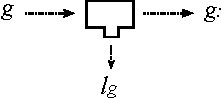
\includegraphics{images/new-label}}%
  \qquad\qquad
  \begin{minipage}{1.2in}%
    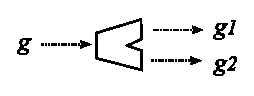
\includegraphics{images/split-gen}
  \end{minipage}%
  \caption{Graphical renderings of $new$ (left) and $split$ (right)}%
  \label{fig:new-and-split}%
\end{figure}



\subsubsection{Model for $new$ and $split$}

The conceptually simplest model of such generators
is one where labels produced are simply the strings of $:$, $1$ and $2$
that designate how the generator was produced from the original root.
For full clarity we show the model here using the full notation.
Both generators and labels are now represented as sequences of the three symbols
$:$, $1$ and $2$.
\RLEQNS{
  s \in LblSym &=& \setof{\texttt{:},\texttt{1},\texttt{2}}
\\ g \in GenSym &=& LblSym^*
\\ l \in Label &=& LblSym^*
\\ new(g) &\defs&  (g,g \cat \seqof{\texttt{:}})
\\ split(g) &\defs&  (g \cat \seqof{\texttt{1}},g \cat \seqof{\texttt{2}})
}
With this model we also get the following law:
For any generator expression $G$,
the following four sets are mutually disjoint:
\[
  \setof{\ell_G}
  \quad
  labs(G_{:})
  \quad
  labs(G_1)
  \quad
  labs(G_2)
  \qquad
  \elabel{labs-fully-disjoint}
\]
This is stronger than we require, but this is not a problem.
We also get three very significant benefits from this model/notation:
\begin{enumerate}
  \item
    It is very easy to decide if two generator expressions
    denote the same label---they do if and only if the expressions are the
    same, which in shorthand terms means the label sequences are the same.
  \item
    It is almost as easy to decide if two generator expressions produce
    disjoint labels.
    This occurs if and only if neither of the sequences of postfix operators
    involved are a prefix of the other.
    Or put differently, a generator's labels are a subset of another's
    iff its postfix sequence extends that of the other generator:
    \RLEQNS{
       labs(\g{\rho}) \subseteq labs(\g{\varrho}) &\equiv& \varrho \leq \rho
       & \elabel{prefix-lab-subset}
    }
    where $\leq$ is the sequence prefix relation.
  \item
    We refer to $g$ as the ``root'' in double quotes,
    because $g$ is not privileged in any way.
    If we substitute a different expression $G$ for $g$
    in the semantics of a construct,
    the behaviour is unchanged.
    In effect $g$ is like a ``base address'',
    with all the labels generated from $g$ being relative to it,
    and replacing $g$ by $G$ simply relocates it and the labels it generates.
    This is the basic mechanism used to construct the semantics
    of all the composite constructs in the language.
\end{enumerate}


\subsection{Label-Set Invariants}

The semantics we propose here depends on the careful management
of when specific labels are, or are not,
present in the global label-set $ls$.
We are looking at a situation where the semantics of any construct
requires associating unique labels with its entry and exit points,
as well as having a label generator provided for use with any sub-components
it might have.

So, from the perspective of any well-program $P$,
we have the following three (static) observation variables.
\RLEQNS{
   in, out &:& Lbl
\\ g &:& Gen
}
Key to the success of this semantics is a collection of label-set invariants
which characterise proper label-set contents,
which are preserved by all label-set manipulations performed
by our semantic definitions.

\subsubsection{Disjoint Labels (DL)}\label{sssec:disjoint-labels}

The first invariant we have is simply one that asserts,
for every construct, that $in$, $out$ and the labels of $g$
are all different
\footnote{The theory can be developed using only $g$ as a static observation,
and letting $\ell_g$ and $\ell_{g:}$ play the role of $in$ and $out$
respectively, in which case Disjoint Labels is automatically satisfied.
However, while this results in an entirely equivalent theory,
it is notationally much more obscure
with definitions and results that are harder to interpret and check.
}%
\RLEQNS{
   in \neq out &\land& \setof{in,out} \cap labs(g) = \emptyset
   & \ecite{Disjoint-Labels}
}



\subsubsection{Label Exclusivity (LE)}\label{sssec:label-exclusivity}

In addition to Disjoint Labels above,
which merely ensures distinctness of labels themselves,
we also need stronger invariants regarding which labels can, or cannot,
occur in the global label set at any one time.
There is not one such Label Exclusivity invariant,
but rather we have that each language construct defines it own
variation, in order to ensure that flow of control is correctly managed.

There is a general version of the invariant, as follows:
\RLEQNS{
   &&
   in \in  ls \implies (\setof{out} \cup labs(g))\cap ls = \emptyset
\\ &\land&
   (labs(g) \cap  ls \neq \emptyset) \implies \setof{in,out}\cap ls = \emptyset
\\ &\land&
   out \in ls \implies (\setof{in} \cup labs(g))\cap ls = \emptyset
   & \ecite{Exclusive-Labels}
}

We also more specific invariants, specific to each composite language construct.
We start with one of the simplest,
namely that used by sequential composition.
It asserts that any point in time,
only one of $in$, $\ell_g$ or $out$ can be present in $ls$:
\RLEQNS{
   &&
   in \in  ls \implies \setof{\ell_g,out}\cap ls = \emptyset
\\ &\land&
   \setof{\ell_g} \subseteq ls \implies \setof{in,out}\cap ls = \emptyset
\\ &\land&
   out \in ls \implies \setof{in,\ell_g}\cap ls = \emptyset
}
The most complex example is that for parallel composition.
Here we have four labels in addition to $in$ and $out$,
namely $\ell_{g1}$, $\ell_{g1:}$, $\ell_{g2}$, and $\ell_{g2:}$.
They should not occupy $ls$ at the same time as either $in $ or $out$,
but we also have that only one of the pair $(\ell_{g1},\ell_{g1:})$
can be present at the same time,
and the same must hold  for $(\ell_{g2},\ell_{g2:})$.
\RLEQNS{
   &&
   in \in ls
   \implies
   \setof{\ell_{g1},\ell_{g1:},\ell_{g2},\ell_{g2:},out}\cap ls = \emptyset
\\ &\land&
   \ell_{g1} \in ls \implies \setof{in,\ell_{g1:},out}\cap ls = \emptyset
\\ &\land&
   \ell_{g1:} \in ls \implies \setof{in,\ell_{g1},out}\cap ls = \emptyset
\\ &\land&
   \ell_{g2} \in ls \implies \setof{in,\ell_{g2:},out}\cap ls = \emptyset
\\ &\land&
   \ell_{g2:} \in ls \implies \setof{in,\ell_{g2},out}\cap ls = \emptyset
\\ &\land&
   out \in ls
   \implies
   \setof{in, \ell_{g1},\ell_{g1:},\ell_{g2},\ell_{g2:}}\cap ls = \emptyset
}
The precise motivation for these will be explained when the relevant
construct semantics are being described later.
For now we simply observe,
that these invariants are quite bulky and complex.



\subsubsection{Label-Set Invariant Notation}

First we shorten $labs(g)$ to just $g$ when this is clear from context,
i.e., a label-set, rather than a generator, is expected.

The Disjoint Labels invariant basically asserts
that a number of sets of labels are mutually disjoint.
We use the following shorthand, where the $L_i$ are label-sets,
\RLEQNS{
   \setof{L_1|L_2|\dots|L_n}
   &\defs&
   \forall_{i,j \in 1\dots n}
    @
    i \neq j \implies L_i \cap L_j = \emptyset
\\ \multicolumn{3}{c}{\elabel{short-disj-lbl}}
}
So we have an alternative definition of the Disjoint Labels invariant:
\RLEQNS{
 && \setof{in|g|out} & \elabel{Disjoint-Labels}
}

In a similar vein, we use a similar shorthand notation
for the Label Exclusivity invariants.
We use a shorthand,
whose easy cases can be formulated as follows:
\RLEQNS{
   ~[L_1|L_2|\dots|L_n]
   &\defs&
   \forall_{i,j \in 1\dots n}
    @
    i \neq j \implies
     ( L_i \cap ls \neq \emptyset \implies L_j \cap ls = \emptyset )
\\ \multicolumn{3}{c}{\elabel{short-lbl-exclusive}}
}
So the sequential composition Label Exclusivity invariant
is simply: $[in|\ell_g|out]$.
What needs to be kept in mind regarding this shorthand notation
is that $ls$ is mentioned under the hood,
and it is really all about what can be present in the global label-set
at any instant in time.

For parallel composition, we a little more complexity.
In shorthand it is expressed as
\[
   [in|(\ell_{g1}|\ell_{g1:}),(\ell_{g2}|\ell_{g2:})|out].
\]
It asserts at the top-level that $ls$
may contain only $in$, only $out$,
or only labels in $\ell_{g1},\ell_{g1:},\ell_{g2},\ell_{g2:}$.
In addition however, $\ell_{g1}$ and $\ell_{g1:}$ cannot occur together
and neither can $\ell_{g2}$ and $\ell_{g2:}$.

A more detailed and formal description of this way of describing
these invariants, in terms of an different abstract notation,
is presented in \S\ref{ssec:exclusive-lsat}.

\subsubsection{Properties of DL and LE}

Consider the following two generic examples:
\begin{enumerate}
  \item
    $DL_n = [L_1|L_2|\dots|L_n]$
    asserts that each $L_i$ is disjoint from any other.
  \item
    $LE_n = \{L_1|L_2|\dots|L_n\}$
    asserts that if elements one $L_i$ are in $ls$,
    then no elements from the others are.
\end{enumerate}

The ordering in either invariant is immaterial.
If $\rho$ is a permutation over $\setof{1\dots n}$ then
\RLEQNS{
   \{L_1|L_2|\dots|L_n\} &=& \{L_{\rho1}|L_{\rho2}|\dots|L_{\rho n}\}
   & \elabel{DL-perm}
\\ ~[L_1|L_2|\dots|L_n] &=& [L_{\rho1}|L_{\rho2}|\dots|L_{\rho n}]
   & \elabel{LE-perm}
}
Both invariants imply shorter versions of themselves:
\RLEQNS{
   \{\dots|L_{i-1}|L_i|L_{i+1}\dots\} &\implies& \{\dots|L_{i-1}|L_{i+1}\dots\}
   & \elabel{DL-drop}
\\ ~[\dots|L_{i-1}|L_i|L_{i+1}\dots] &\implies& [\dots|L_{i-1}|L_{i+1}\dots]
   & \elabel{LE-drop}
}
Both invariants imply versions with smaller sets:
\RLEQNS{
   S_i \subseteq L_i \land \{L_1|\dots|L_n\}
   &\implies& \{S_1|\dots|S_n\}
   & \elabel{DL-subset}
\\ S_i \subseteq L_i \land [L_1|\dots|L_n]
   &\implies& [S_1|\dots|S_n]
   & \elabel{DL-subset}
}
A key property shared by all LE invariants,
is that they are trivially satisfied by $ls = \emptyset$,
or if $ls$ only contains labels not mentioned in the invariant.
\RLEQNS{
   scope(LE_n) &\defs& L_1 \cup L_2 \cup \dots \cup L_n
\\ (ls = ls \setminus scope(LE_n)) &\implies& LE_n = \true
    & \elabel{LE-out-of-scope}
\\ ls = \emptyset &\implies& LE_n = \true
    & \elabel{LE-trivial}
}
There is no simple relationship between $DL_n$ and $LE_n$.
It is possible for one to be true when the other is false.
\begin{description}
  \item[DL true, LE false]
    $L_1 \cap L_2 = \emptyset \quad\land\quad (L_1 \cup L_2) \subseteq ls$.
  \item[DL false, LE true]
    $L_1 = L_2 \quad\land\quad L_1 \cap ls = \emptyset$
\end{description}

%\newpage
%\section{Denotations}\label{sec:denote}

\subsection{Overview}


Concurrent programs are a mix of control constructs ($\cseq,\parallel,+,\dots$)
and atomic actions $a$ that modify \emph{program state} $s$.
This is all that is visible to the programmer.



Our denotational UTP semantics
is inspired by that done for UTPP\cite{DBLP:conf/icfem/WoodcockH02},
itself based on a UTP theory of \emph{action systems}.
First, we add a new state component, not visible in the program text,
which is a set of labels ($ls$).
These labels are used to orchestrate the flow of control.
Given an atomic action $a$ that only knows about program state $s$,
we use notation $\catom a$ to describe a lifted version
of $a$ that takes account of the contents of the label-set $ls$.
In effect a lifted atomic state action is disabled until
a particular label is present in that set.
A disabled action does not modify the state any way
and simply monitors the label-set.
Once an action observes the presence/arrival of its label,
it then becomes active.
An active lifted action $\catom a$ atomically modifies the extended state as follows:
\begin{itemize}
  \item It makes the changes to $s$ as determined by its underlying action $a$.
  \item It removes the enabling label from the label-set.
  \item It adds in appropriate ``continuation'' labels to $ls$.
\end{itemize}
In \cite{DBLP:conf/icfem/WoodcockH02},
the language syntax required explicit (starting) labels
for every atomic state change action,
and these are used as lifted action enablers.
The continuation labels were taken to the the enabling labels
of whatever other actions occurred immediately after, in the program.
This means that the resulting semantics is not compositional.

The approach we adopt is to adopt the notion of \emph{label generators}
to create the labels, so ensuring they are unique,
but in such a way as make the generation a compositional process.
In addition we explicitly associate two labels with every program construct:
one that marks the entry into the construct,
and another that indicates the exit.

\subsubsection{On Notation}

We make liberal use of a number of shorthand notations,
largely to reduce expression size and clutter.
Typically these reduce the use of infix operators,
and in one notable case, collapse large conjunctions
of implications into a simple form with string visual cues.
Each shorthand is introduced by a subsection similar to this one.

\subsection{Label Generation}

INTRODUCE

\RLEQNS{
   g &:& Gen = \setof g  & \mbox{only one variable!}
\\ \ell &:& Gen \fun Lbl
\\ G \in Gen &::=&  g     & \mbox{the ``root'' generator}
\\           &\mid& G_{:} & \mbox{resulting generator after label produced}
\\           &\mid& G_1   & \mbox{first generator after generator split}
\\           &\mid& G_2   & \mbox{second generator after generator split}
\\ L \in Lbl &::=& \ell_G & \mbox{label produced by generator}
}
Note that our generator expression language has only one variable, $g$,
which denotes the ``root'' generator.
All generator expressions have the form $g$ followed by zero
or more uses of $:$, $1$ and $2$.
We say the  ``root'' generator because this notion is local to a
particular context, and we can relativise things by replacing $g$
by an arbitrary $G$ expression.
We define the notion of the set of labels produced by a generator,
which must satisfy the following laws:
\RLEQNS{
   labs &:& Gen \fun \power Lbl
\\ labs(G) &=& \setof{\ell_G} \cup labs(G_{:}) \cup labs(G_1) \cup labs(G_2)
  &\elabel{labs-def}
\\ \ell_G &\notin& labs(G_{:})
   &\elabel{labs-unique}
\\ \emptyset &=& labs(G_1) \cap labs(G_2)
  &\elabel{labs-split-disjoint}
}
The conceptually simplest model of such a generator
is one where labels are simply the strings of $:$, $1$ and $2$
that designate how its generator was produced from the root.
With this model we also get the following law:
For any generator expression $G$,
the following four sets are mutually disjoint:
\[
  \setof{\ell_G}
  \quad
  labs(G_{:})
  \quad
  labs(G_1)
  \quad
  labs(G_2)
  \qquad
  \elabel{labs-fully-disjoint}
\]

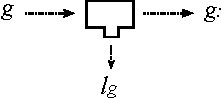
\includegraphics{images/new-label}

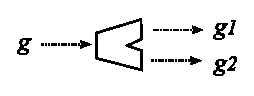
\includegraphics{images/split-gen}


\subsection{Observation Variables}

\begin{eqnarray*}
   s, s' &:& \mathcal S
\\ ls, ls' &:& \mathcal P (Lbl)
\\ g &:& Gen
\\ in, out &:& Lbl
\end{eqnarray*}
We assume a general notion of expressions ($e$)
and say that an expression $e$ is ``ground''
if it's free variables are limited to only $g$, $in$ and $out$.


\subsection{Label-Set Invariants}


We want to distinguish between disjointness only:
\[ \{ in | g | out \} \]
from disjointness with label-set exclusion:
\[ [ in | g | out ] \]

We want to be able to specify that certain combinations
of labels should never appear simultaneously
in the global label set ($ls$).
We do this by defining a label-set invariant $I$
which has alphabet $ls,in,out,g$.

We start by defining a general abstract way of specifying
sets with valid combinations
of values drawn from a parameter type $\tau$.
\RLEQNS{
   i \in I_\tau &::=& \tau   &  \mbox{can contain this value}
\\ &\mid& \otimes(i,\ldots,i) & \mbox{at most one of these allowed to contain}
\\ &\mid& \cup (i,\ldots,i) & \mbox{any of these allowed to contain}
}

We define what it means for an atomic action invocation
to satisfy an invariant parameterised on the label type ($Lbl$).
\RLEQNS{
  ls \textbf{ lsat } I \land A(E|a|N) &\implies& ls' \textbf{ lsat } I
}
We can re-formulate this as a following equivalent test:
\RLEQNS{
   A(E|a|N) \textbf{ sat } I_{Lbl}
   &\defs&
   E \textbf{ lsat } I_{Lbl} \land N \textbf{ lsat } I_{Lbl}
}
In effect we identify the occurrences of labels within this $I$-structure,
and then check the multiplicity constraints:
\RLEQNS{
   L \textbf{ lsat } I_{Lbl} &\defs& res=ok
\\ \textbf{where} && (res,\_) = occChk (occ_L I_{Lbl})
}
The $occ$ function takes a set $L$ of $\tau$ and an $I_\tau$ and returns a $I_\Bool$
that records if the corresponding element of $\tau$ is present in $L$.
\RLEQNS{
   occ &:& \power \tau \fun I_\tau \fun I_\Bool
\\ occ_L~\ell &\defs& \ell \in L
\\ occ_L~\otimes(i_1,\ldots,i_n)
   &\defs&
   \otimes(occ_L~i_1,\ldots,occ_L~i_n)
\\ occ_L~\cup(i_1,\ldots,i_n)
   &\defs&
   \cup(occ_L~i_1,\ldots,occ_L~i_n)
}
The $occChk$ function pattern matches across the boolean values to see if
constraints are satisfied.
The first component of the result is an overall ok/fail indicator,
while the second boolean component indicates if values are present
in any component.
\RLEQNS{
   occChk &:& I_\Bool \fun (\setof{ok,fail}\times \Bool)
\\ occChk(b) &\defs& (ok,b)
\\ occChk(\cup(i_1,\ldots,i_n))
   &\defs&
   (fail,\_),
   \textbf{ if }\exists j @ occChk(i_j) = (fail,\_)
\\ && (ok,b_1 \lor \dots \lor b_n),
   \textbf{ if }\forall j @ occChk(i_j) = (ok,b_j)
\\ occChk(\otimes(i_1,\ldots,i_n))
   &\defs&
   (fail,\_),
   \textbf{ if }\exists j @ occChk(i_j) = (fail,\_)
\\&& (fail,\_) \mbox{ if more than one $(ok,true)$}
\\&& (ok,false) \mbox{ if all are $(ok,false)$}
\\&& (ok,true) \mbox{ if  exactly one $(ok,true)$}
}
We note, as a consequence of the above definitions, that
\RLEQNS{
  \emptyset &  \textbf{lsat} &  I & \elabel{emp-lsat-I}
}
for any label-set invariant $I$.

We introduce a shorthand for invariants illustrated as follows.
\RLEQNS{
  ~ [ a,b,c | d,e | f ]
   &=&
   ls \textbf{ lsat } \otimes(\cup(a,b,c),\cup(d,e),f)
\\ ~[ a | (b|c),(d|e) | f ]
  &=&
  ls \textbf{ lsat } \otimes(a,\cup(\otimes(b,c),\otimes(d,e)),f)
}
In effect we make the involvement of $ls$ implicit,
and use bar ($|$) and comma ($,$) to replace $\otimes$ and $\cup$ respectively.
We also have a shorthand that just denotes
the non-intersecting nature of the arguments.
E.g.,
$\setof{A|B|C}$ asserts that $A$, $B$ and $C$ are mutually disjoint,
without any reference to $ls$ or any other set.

\subsubsection{Invariant Examples}

The following examples show how various instances of $ls \textbf{ lsat } I$
get expanded:
\RLEQNS{
   ~[in|out]
   &=&
   \setof{in} \cap \setof{out} = \emptyset
\\ &\land&
  \setof{in} \subseteq ls \implies \setof{out}\cap ls = \emptyset
\\ &\land&
  \setof{out} \subseteq ls \implies \setof{in}\cap ls = \emptyset
\\
\\ ~[in|\ell|out]
   &=&
   \setof{in} \cap \setof{\ell,out} = \emptyset
\\ &\land&
   \setof{\ell} \cap \setof{in,out} = \emptyset
\\ &\land&
   \setof{out} \cap \setof{in,\ell} = \emptyset
\\ &\land&
  \setof{in} \subseteq ls \implies \setof{\ell,out}\cap ls = \emptyset
\\ &\land&
  \setof{\ell} \subseteq ls \implies \setof{in,out}\cap ls = \emptyset
\\ &\land&
  \setof{out} \subseteq ls \implies \setof{in,\ell}\cap ls = \emptyset
\\
\\ ~[ a | (b|c),(d|e) | f ]
   &=&
   \setof{a} \cap \setof{b,c,d,e,f} = \emptyset
\\ &\land&
   \setof{b,c,d,e} \cap \setof{a,f} = \emptyset
\\ &\land&
   \setof{f} \cap \setof{a,b,c,d} = \emptyset
\\ &\land&
  \setof{a} \subseteq ls \implies \setof{b,c,d,e,f}\cap ls = \emptyset
\\ &\land&
  \setof{b,c,d,e} \subseteq ls \implies \setof{a,f}\cap ls = \emptyset
\\ &\land&
  \setof{f} \subseteq ls \implies \setof{a,b,c,d,e}\cap ls = \emptyset
\\ &\land&
   \setof{b} \cap \setof{c} = \emptyset
\\ &\land&
   \setof{d} \cap \setof{e} = \emptyset
\\ &\land&
  \setof{b} \subseteq ls \implies \setof{c}\cap ls = \emptyset
\\ &\land&
  \setof{c} \subseteq ls \implies \setof{b}\cap ls = \emptyset
\\ &\land&
  \setof{d} \subseteq ls \implies \setof{e}\cap ls = \emptyset
\\ &\land&
  \setof{e} \subseteq ls \implies \setof{d}\cap ls = \emptyset
}
Here one of $b$ or $c$ may occur in $ls$ along with one of  $d$ or $e$.
In this theory,
we use the label generators to ensure that the disjointness
conditions of the invariants are always true, by construction.

\subsubsection{Notation}

\RLEQNS{
   ls(\ell) &\defs& \ell \in ls
\\ ls(L) &\defs& L \subseteq ls
\\ ls(\B\ell) &\defs& \ell \notin ls
\\ ls(\B L) &\defs& L \cap ls = \emptyset
}



\subsection{``Standard'' UTP Predicates}

INTRODUCE

\RLEQNS{
   P \cond C Q
   &\defs&
   C \land P \lor \lnot C \land Q
   & \elabel{UTP-cond-def}
\\ \Skip
   &\defs&
   s'= s \land ls'=ls
   & \elabel{UTP-skip-def}
\\ P \seq Q
   &\defs& \exists s_m,ls_m \bullet
\\ && \qquad P[s_m,ls_m/s',ls'] \land Q[s_m,ls_m/s,ls]
   & \elabel{UTP-seq-def}
\\ C * P
   &=&
   P ; C * P \cond C \Skip
   & \elabel{UTP-loop-unroll}
}
We also define a specialised form of sequential composition
to be used when neither component refers to $ls$ or $ls'$,
and its unit:
\RLEQNS{
   P \seq_s Q
   &\defs&
   \exists s_m \bullet P[s_m/s'] \land Q[s_m/s]
   & \elabel{UTP-s-seq-def}
\\ ii &\defs& s'=s & \elabel{ii-def}
}
Note that if neither predicate mentions $ls$ or $ls'$
then the effect of $\seq$ and $\seq_s$ is the same.
We often omit the $s$ subscript when its use is clear from context.

\subsection{Healthiness Conditions}

\subsubsection{Disjoint Labels}

We have a general healthiness condition (Disjoint Labels) which asserts
that the labels associated with $in$, $out$ and $g$
are different:
\RLEQNS{
  \DL(P) &=& P \land in \neq out \land \setof{in,out} \cap labs(g) = \emptyset
}

\subsubsection{Wheels-within-Wheels}

The key intuition behind this compositional semantics was to take the
$run$ function of the action-system based semantic model used in UTPP,
and drive it inwards to every level of the program.
The original $run$ can be defined in the context of this theory as
\[
  run(P) = ls := \setof{in} ; \lnot (out \in ls) * P
\]
However this failed to keep atomic components ``live''.
They could never be re-executed,
as would be required if they were within an iteration.
Instead it was realised that every construct (atomic and composite)
would have to be within an infinite loop.
\RLEQNS{
   \W(P) &\defs& \true * P &\elabel{W-as-loop}
}
This bold step turns out to be remarkably effective,
with some quite counter-intuitive outcomes.
However it does depend on a specific tweak to the
definition of an atomic action.
In effect we define an atomic action
as placing a basic action inside such a loop,
but within a non-deterministic choice between it
and a \emph{stuttering} step, denoted by UTP skip:
\RLEQNS{
  \catom a &\defs& \W(\Skip \lor A(in|a|out))
}
A result of this is that this stuttering step gets
propagated up to enclosing composites,
so in effect we see $\W(C)=\W(\Skip\lor C)$
where $C$ is any predicate denoting the semantics of a command.
We give more details about this in the section on calculation (\S\ref{sec:calc}).
One key calculational advantage of this is that we can rewrite
the rhs of the definition of $\W$ as:
\RLEQNS{
   \W(P) &  =  & \bigvee_{i \in 0,\dots} \Skip \seq P^i &\elabel{W-as-NDC}
}%
We note explicitly here that, in effect,
our semantic model is based on unbounded non-determinism.

However, for iteration-free programs
we find that there is a finite $k$ such that $P^k = \false$,
in which case the non-determinism is bounded.
We get these finite results that seem very similar
to the results obtained by using $run$ above.
Using $run$ results in predicates that cannot be composed
to get composite behaviour.
However, using $\W$ results in a slight variation,
which is composable!
What turns out to be crucial
to this outcome is the explicit stuttering option in the infinite loop.

\subsubsection{Mumble Closure}

A program's semantics includes all its mumblings,
and so should be unchanged if sequentially composed with itself
using \emph{UTP} sequential composition:
\RLEQNS{
   P \seq P &=& P  & \eref{mumble-closure}
}

\subsection{UTP Denotational Semantics}

INTRODUCE

We present each construct individually,
with full diagrams for each \dots



\subsubsection{Basic Action}

Basic Action $A(E|a|N)$ is enabled when all the labels in $E$
are present in the global label-set
and atomic action $a$ does not evaluate to $\false$
in the current program state.
If so enabled,  it performs action $a$, removes the labels in $E$
from the label-set, and adds in those in $N$.
\RLEQNS{
   A(E|a|N)
   &\defs&
   ls(E) \land a \land ls'=(ls\setminus E) \cup N
   & \elabel{A-def}
}




\newpage
\subsubsection{Atomic Action}

\includegraphics{images/atomic-action}
\RLEQNS{
  \catom a
  &\defs& \DL(\W(\Skip \lor A(in|a|out))) & \elabel{sem:atomic}
\\ &=&  [in|out] \land (\Skip \lor A(in|a|out))
        & \elabel{nf-atomic}
}

Invariant Preservation:
\RLEQNS{
   [in|out]\gamma \land A(in|a|out)\gamma &\implies& [in|out]'\gamma
   & \elabel{atom-inv-ok}
}

\subsubsection{Guarded Atomic Action}
In effect there is no real difference between $c \pgrd a$
and $\true \pgrd (c \land a)$,
so in fact we don't need guarded actions as basic.
This is an advantage of treating the atomic action as a relational predicate
on state.

\RLEQNS{
 c \pgrd a &\defs& \catom{c \land a}  &\elabel{sem:pgrd}
}


\subsubsection{Skip}

\RLEQNS{
   ii     &\defs& s'=s
\\ \cskip &\defs& \catom{ii}  &\elabel{sem:skip}
\\  &=&  [in|out] \land (\Skip \lor A(in|ii|out))
    &\elabel{nf-skip}
}

\newpage
\subsubsection{Sequential Composition}

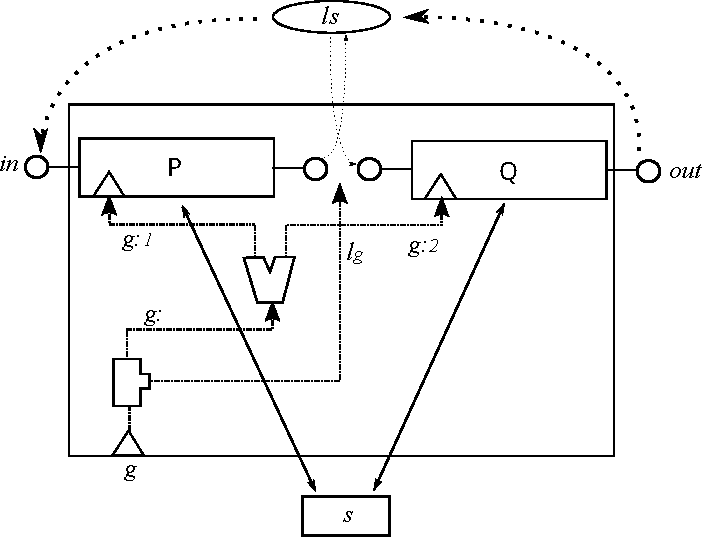
\includegraphics{images/seq-comp-actual}

\RLEQNS{
   P \cseq Q
   &\defs&
   [in|\ell_g|out]\land \W(P[g_{:1},\ell_g/g,out] \lor Q[g_{:2},\ell_g/g,in])
   & \elabel{sem:seq}
}

If $A$ actions in $P$ and $Q$ preserve the invariant,
then so does their composition.
This is immediate by the ground/sound substitution independence
of invariant preservation.



\newpage
\subsubsection{Parallel Composition}

\RLEQNS{
   P \parallel Q
   &\defs&
   [in|(\ell_{g1}|\ell_{g1:}),(\ell_{g2}|\ell_{g2:})|out] \land {}
   & \elabel{sem:par}
\\&& \W(\quad\phlor A(in|ii|\ell_{g1},\ell_{g2})
\\ && \qquad {}\lor
   P[g_{1::},\ell_{g1},\ell_{g1:}/g,in,out]
\\ && \qquad {}\lor
    Q[g_{2::},\ell_{g2},\ell_{g2:}/g,in,out]
\\ && \qquad {}\lor
   A(\ell_{g1:},\ell_{g2:}|ii|out)~)
}

\includegraphics{images/parallel-label-gen}

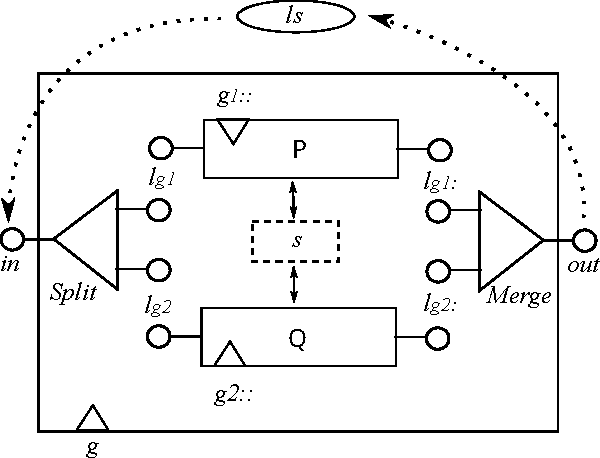
\includegraphics{images/par-comp-actual}


\newpage
\subsubsection{Nondeterministic Choice}

\RLEQNS{
   P + Q
   &\defs&
   [in|\ell_{g1}|\ell_{g2}|out] \land {}
   & \elabel{sem:NDC}
\\ && \W(\quad {}\phlor A(in|ii|\ell_{g1})
\\ && \qquad {} \lor
                     A(in|ii|\ell_{g2})
\\ && \qquad {} \lor
   P[g_{1:},\ell_{g1}/g,in]
\\ && \qquad {} \lor
   Q[g_{2:},\ell_{g2}/g,in]~)
}

\subsubsection{Nondeterministic Loop}


\RLEQNS{
   P^*
   &\defs&
   [in|\ell_g|out] \land {}
   & \elabel{sem:star}
\\ && \W(\quad  \phlor A(in|ii|out)
\\ && \qquad {}\lor A(in|ii|\ell_g)
\\ && \qquad {}\lor P[g_{:},\ell_g,in/g,in,out]~)
}

\newpage
\subsubsection{Conditional Choice}

\RLEQNS{
   P \dcond c Q
   &\defs&
   [in|\ell_{g1}|\ell_{g2}|out] \land {}
   & \elabel{sem:cond}
\\ && \W(\quad {}\phlor A(in|c \land ii|\ell_{g1})
\\ && \qquad {} \lor
                     A(in|\lnot c \land ii|\ell_{g2})
\\ && \qquad {} \lor
   P[g_{1:},\ell_{g1}/g,in]
\\ && \qquad {} \lor
   Q[g_{2:},\ell_{g2}/g,in]~)
}

\includegraphics{images/conditional-actual}

\newpage
\subsubsection{Conditional Loop}


\RLEQNS{
   c \ddo P
   &\defs&
   [in|\ell_g|out] \land {}
   & \elabel{sem:iter}
\\ && \W(\quad  \phlor A(in|\lnot c \land ii|out)
\\ && \qquad {}\lor A(in|c \land ii|\ell_g)
\\ && \qquad {}\lor P[g_{:},\ell_g,in/g,in,out]~)
}

\includegraphics{images/iteration-actual}

\newpage
\subsection{Essential Properties?}

The first key property is that every instance of $A$
in the semantics preserves the invariant.

Looking forward we will want some key algebraic properties:
\RLEQNS{
   ~[S_1|\dots|S_n]
   &=&
   [S_{\rho(1)}|\dots|S_{\rho(n)}]
\\ && \rho \textrm{ a permutation of } 1\dots n
\\ ~[S_1|\dots|S_i|S_{i+1}|\dots|S_n]
   &\implies&
   [S_1|\dots|S_i]
   ,\quad i > 1 &\elabel{I-subsumption}
\\ ~[S_1|\dots|S_n]\gamma &=& [S_1\gamma|\dots|S_n\gamma]
   & \elabel{I-gamma-subst}
\\ A(E|a|N)\gamma &=& A(E\gamma|a|N\gamma)
\\ A(E|a|N) \textbf{ sat } I
   &=&
   A(E|a|N)\gamma \textbf{ sat } I\gamma
   , \quad \mbox{arbitrary }\gamma
\\ ((ls\setminus R)\cup A)(S)
   &=&
   ls(F(R,A,S)) \land P(R,A,S)
\\ \Skip \seq P &=~P~=& P \seq \Skip
\\ (P\seq Q)\gamma &=& P\gamma \seq Q\gamma  & \elabel{seq-gnd-distr}
\\ \Skip\gamma &=& \Skip
\\ \W(P)  && \textrm{monotonic in } P
\\ \W(\W(P)) &=& \W(P) & ?
\\ \W(\W(\Skip \lor P)) &=& \W(\Skip \lor P)
\\ \W(\Skip \lor P) &=& \bigvee_{i \in 0,\dots} \Skip \seq P^i
   & \elabel{W-as-NDC}
\\ \W(P)\gamma &=& \W(P\gamma) & \elabel{W-gamma-subst}
\\ \W(\Skip \lor P) &=& \Skip \lor \W(\Skip \lor P)
\\ I \land \W(P) &=& \W(I \land P) & \elabel{I-W-distr}
}

When $P\gamma$ executes:
\begin{description}
  \item[\elabel{P-removes-in}]
    it will remove $in\gamma$ from $ls$ at some point;
  \item[\elabel{P-removes-g}]
    the only other labels it removes are in $labs(g\gamma)$;
  \item[\elabel{P-adds-out}]
    it adds $out\gamma$ into $ls$ at some point;
  \item[\elabel{P-adds-g}]
    the only other labels it adds are in $labs(g\gamma)$;
  \item[\elabel{P-ignores-rest}]
    and its behaviour is not affected by any label not
    in
    \\$\setof{in\gamma,out\gamma} \cup labs(g\gamma)$.
\end{description}
We can summarise this as follows:
\begin{itemize}
  \item $P\gamma$ actions are enabled by labels in $in\gamma,g\gamma$
  \item $P\gamma$ actions enable actions enabled by $g\gamma,out\gamma$
  \item Remember that the following invariant holds: $[in\gamma|g\gamma|out\gamma]$
\end{itemize}




\newpage
\subsection{Miscellaneous}

Most of this stuff should end up,
if required,
in a Proofs/Justification appendix.

\subsubsection{Semantic Substitutions List}

It can be informative to see the invariants grouped with
the relevant actions and substitutions.
\RLEQNS{
   ~[in|out]
   && A(in|a|out)
\\ && id
\\
\\ ~[in|\ell_g|out]
   && [g_{:1},\ell_g/g,out]
\\ && [g_{:2},\ell_g/g,in]
\\
\\ ~[in|(\ell_{g1}|\ell_{g1:}),(\ell_{g2}|\ell_{g2:})|out]
   && A(in|ii|\ell_{g1},\ell_{g2})
\\ && A(\ell_{g1:},\ell_{g2:}|ii|out)
\\ && [g_{1::},\ell_{g1},\ell_{g1:}/g,in,out]
\\ && [g_{2::},\ell_{g2},\ell_{g2:}/g,in,out]
\\
\\ ~[in|\ell_{g1}|\ell_{g2}|out]
   && A(in|ii|\ell_{g1})
\\ && A(in|ii|\ell_{g2})
\\ && [g_{1:},\ell_{g1}/g,in]
\\ && [g_{2:},\ell_{g2}/g,in]
\\
\\ ~[in|\ell_g|out]
   && A(in|ii|out)
\\ && A(in|ii|\ell_g)
\\ && P[g_{:},\ell_g,in/g,in,out]
\\
\\ ~[in|\ell_{g1}|\ell_{g2}|out]
   && A(in|c \land ii|\ell_{g1})
\\ && A(in|\lnot c \land ii|\ell_{g2})
\\ && [g_{1:},\ell_{g1}/g,in]
\\ && [g_{2:},\ell_{g2}/g,in]
\\
\\ ~[in|\ell_g|out]
\\ && A(in|\lnot c \land ii|out)
\\ && A(in|c \land ii|\ell_g)
\\ && [g_{:},\ell_g,in/g,in,out]
}

\subsubsection{Nested Invariants}

For each composite,
we show how its component substitutions affect their invariants
and any entailment relationships that arise.
We don't show the conditional variants of choice and iteration
because their invariants and substitutions are the same as those
in the corresponding non-deterministic constructs.

Semantics Reminder:
\RLEQNS{
  \catom a
  &\defs& [in|out] \land \W(\Skip \lor A(in|a|out))
\\ P \cseq Q
   &\defs&
   [in|\ell_g|out]\land \W(P[g_{:1},\ell_g/g,out] \lor Q[g_{:2},\ell_g/g,in])
\\ P \parallel Q
   &\defs&
   [in|(\ell_{g1}|\ell_{g1:}),(\ell_{g2}|\ell_{g2:})|out] \land {}
\\&& \W(\quad\phlor A(in|ii|\ell_{g1},\ell_{g2})
\\ && \qquad {}\lor
   P[g_{1::},\ell_{g1},\ell_{g1:}/g,in,out]
\\ && \qquad {}\lor
    Q[g_{2::},\ell_{g2},\ell_{g2:}/g,in,out]
\\ && \qquad {}\lor
   A(\ell_{g1:},\ell_{g2:}|ii|out)~)
\\ P + Q
   &\defs&
   [in|\ell_{g1}|\ell_{g2}|out] \land {}
\\ && \W(\quad {}\phlor A(in|ii|\ell_{g1})
\\ && \qquad {} \lor
                     A(in|ii|\ell_{g2})
\\ && \qquad {} \lor
   P[g_{1:},\ell_{g1}/g,in]
\\ && \qquad {} \lor
   Q[g_{2:},\ell_{g2}/g,in]~)
\\ P^*
   &\defs&
   [in|\ell_g|out] \land {}
\\ && \W(\quad  \phlor A(in|ii|out)
\\ && \qquad {}\lor A(in|ii|\ell_g)
\\ && \qquad {}\lor P[g_{:},\ell_g,in/g,in,out]~)
}


\paragraph{Sequential Composition}

\begin{description}
  \item[Invariant]
    $[in|\ell_g|out]$
  \item[Substitutions]
    $[g_{:1},\ell_g/g,out]$ and $[g_{:2},\ell_g/g,in]$
  \item[Component Invariants]
    $$\begin{array}{|l|c|c|}
    \hline
      \mbox{Type} & \mbox{as }P & \mbox{as }Q
    \\\hline
      \catom\_ & [in|\ell_g] & [\ell_g|out]
    \\\hline
       \_\cseq\_& [in|\ell_{g:1}|\ell_g] & [\ell_g|\ell_{g:2}|out]
    \\\hline
       \_\parallel\_
       & [in|(\ell_{g:11}|\ell_{g:11:}),(\ell_{g:12}|\ell_{g:12:})|\ell_g]
       & [\ell_g|(\ell_{g:21}|\ell_{g:21:}),(\ell_{g:22}|\ell_{g:22:})|out]
    \\\hline
    \end{array}$$
\end{description}
Hmmm \dots, no simple relationship is emerging.

%\newpage
%\section{Semantic Calculations}\label{sec:calc}

\textbf{SHOULD COMPUTE PARTIAL NORMAL FORMS
FOR COMPOSTITES}

\subsection{Composing $A$s}\label{ssec:comp-A}

We have a problem in that actions defined using $A(\dots)$
are not closed under standard UTP sequential composition (\eref{UTP-seq-def}).
We need a more general form,
where the labels removed are not necessarily
exactly those that had to be present to enable the action.
We call this eXtended atomic action $X$ and it is defined as follows:
\RLEQNS{
   X(E|a|R|A)
   &\defs&
   ls(E) \land s' \in \sem a s \land ls' = (ls \setminus R) \cup A
   & \elabel{X-def}
}
We can then re-define $A$ in terms of $X$:
\RLEQNS{
   A(E|a|N)
   &=&
   X(E|a|E|N)
   & \elabel{A-alt-def}
}
The key law is one regarding sequentially composing $X$s:
\RLEQNS{
   \lefteqn{X(E_1|a|R_1|A_1) ; X(E_2|b|R_2|A_2)} &&& \elabel{X-then-X}
\\ &=& (E_2\setminus A_1) \cap R_1 = \emptyset
\\ &\land&
   X(E_1 \cup (E_2\setminus A_1)
       |a\seq b
       |R_1 \cup R_2
       |(A_1 \setminus R_2) \cup  A_2)
}
The condition $(E_2\setminus A_1) \cap R_1 = \emptyset$
characterises all those cases were the second $X$ is enabled
immediately after the first $X$ terminates
(i.e., without any outside interference).

\textbf{ANOTHER IMPORTANT LAW:}
If $(E_1 \cup N_1) \cap (E_2 \cup N_2)$, then
\[
  A(E_1|a|N_1) \seq A(E_2|b|N_2)
  =
  A(E_1\cup E_2|a\seq b|N_1\cup N_2)
\]
(and vice-versa)!

\subsection{Normal Form}\label{sec:normal-form}

All the semantics above have an invariant $I_P$,
zero or more atomic actions ($A_i$),
plus zero or more language sub-component predicates ($P_j$)
assembled into a predicate of the form:
\[
  I_P
  \land
  \W( A_1 \lor \dots \lor A_m
     \lor
     P_1\sigma_1 \lor \dots \lor P_n\sigma_n )
\]
where each $\sigma_i = [G_i,I_i,O_i/g,in,out]$,
with all $G_i$, $I_i$ and $O_i$ being ground
and satisfying the invariant $[I_i|labs(G_i)|O_i]$.

\subsubsection{Stuttering Propagates Up}

We show that for any predicate $P$ resulting from the
semantics applied to a program,
that the stuttering on such a predicate propagates up:
\RLEQNS{
   P &=& \Skip \lor P
}



\subsubsection{Nondeterministic Iteration}

Given that we have,
for predicates $P$ used in program semantic definitions,
that
\[
  \W(P) = \bigvee_{i \in 0\dots} \Skip \seq P^i
\]
we find that the following outcomes result:
\begin{enumerate}
  \item
    Every program $P$ can be transformed,
    in principle at least,
    to the form
    \[
      I_P \land \Skip
      \lor
      \bigvee_{n \in 0\dots}  (I_P \land I_n \land X(E_n|a_n|R_n|A_n) \land S_n)
    \]
    for suitable choices of $I_n$, $E_n$, $a_n$, $R_n$, $A_n$ and $S_n$,
    depending on $P$.
    In particular, we find that the $E_n$ and $A_n$ all satisfy the relevant
    label-set invariants.
  \item
    For any complete program that does not use iteration constructs,
    this expansion is finite.
  \item
    For any complete program the $S_n$
    term in $X(E_n|a_n|R_n|A_n) \land S_n$
    is a ground-expression, and is statically decidable as $\true$ or $\false$.
    If $\true$, we find that the above term
    can be be simplified to one of the form $A(E_n|a_n|A_n)$.
    We do not prove this, but note that we have observed it as a result
    of test calculations and these lead us to believe it is true in general.
\end{enumerate}
\RLEQNS{
   P
   &=&
   I_P \land \Skip
      \lor
      \bigvee_{n \in 0\dots}
      (I_P \land I_n \land X(E_n|a_n|R_n|A_n) \land S_n)
   & \elabel{UTCP-NF}
}
This can be shown by an inductive argument over the language syntax,
noting that the sequential composition of two such forms
can itself be transformed into such a form.
In effect this defines a \emph{normal form} for our semantics.


An important law we shall require is that the UTP sequential
composition of two normal forms can itself be expressed
as such a normal form:
\RLEQNS{
   I \land (\Skip\lor\bigvee A_i) \seq J \land (\Skip\lor\bigvee B_j)
   &=&
   I \land J \land (\Skip\lor\bigvee (A_i \seq B_j))
   &\elabel{nf-seq}
}
This is an easy result of the fact that $\seq$ distributes through $\lor$,
and $\Skip$ is a unit for it as well.


\subsection{Normal Form Results for Atomic components}

We now present the results of calculations of normal forms for every language
construct, given atomic sub-components,
and the generic case.

For ease of reading in the former,
we display the invariant $I$ on the first line,
followed by the list of $A(\dots)$ disjuncts, perhaps several on a line,
as follows
\RLEQNS{
   res &=& I
\\ && A(E_1|a_1|N_1) \quad A(E_1|a_2|N_2)) \quad \dots
}
We omit parentheses, logical operators, and the ever-present $\Skip$.
In general we try to put all the single atomic steps on the first line,
with all the mumblings on lower lines.
Here we also just write $a$ instead of $\catom a$,
for brevity.

In the latter generic case we  \emph{\dots to be determined \dots}

\subsubsection{Atomic Actions}
\RLEQNS{
   a &=& [in|out]
\\ && A(in|a|out) & \elabel{NF:atomic-a}
\\
\\ \cskip &=& [in|out]
\\ && A(in|ii|out) & \elabel{NF-skip}
}

\subsubsection{Sequential Composition}

With atomic components:
\RLEQNS{
   a \cseq b
   &=& [in|\ell_g|out]
\\ && A(in|a|\ell_g)\quad  A(\ell_g|b|out)
\\ && A(in|a\seq b|out)
}

With generic components:
\RLEQNS{
   P \cseq Q
   &=& [in|\ell_g|out]
\\ && A(in|a|\ell_g)\quad  A(\ell_g|b|out)
\\ && A(in|a\seq b|out)
}


\subsubsection{Non-deterministic Choice}
\RLEQNS{
   a + b
   &=& [in|\ell_{g1}|\ell_{g2}|out]
\\ &&  A(in|ii|\ell_{g1}) \quad A(in|ii|\ell_{g2})
       \quad
       A(\ell_{g1}|a|out) \quad A(\ell_{g2}|b|out)
\\&& A(in|a|out) \quad A(in|b|out)
}


\subsubsection{Parallel Composition}
Here $\#n$ denotes mumblings of length $n$.
\RLEQNS{
   a \parallel b
   &=& [in\mid([\ell_{g1}|\ell_{g1:}],[\ell_{g2}|\ell_{g2:}])\mid out]
\\ &&  A(in|ii|\ell_{g1},\ell_{g2})
       \quad
       A(\ell_{g1:},\ell_{g2:}|ii|out)
       \quad
       A(\ell_{g1}|a|\ell_{g1:})
       \quad
       A(\ell_{g2}|b|\ell_{g2:}) &
\\ && A(in|a|\ell_{g1:},\ell_{g2})
      \quad
      A(\ell_{g1},\ell_{g2}|b;a|\ell_{g1:},\ell_{g2:})
      \quad
      A(in|b|\ell_{g2:},\ell_{g1}) & \#2
\\ && A(\ell_{g1},\ell_{g2}|a ; b|\ell_{g1:},\ell_{g2:})
      \quad
      A(\ell_{g2:},\ell_{g1}|a|out)
      \quad
      A(\ell_{g1:},\ell_{g2}|b|out) & \#2
\\ && A(in|b;a|\ell_{g1:},\ell_{g2:})
      \quad
      A(in|a;b|\ell_{g1:},\ell_{g2:}) & \#3
\\ && A(\ell_{g1},\ell_{g2}|b;a|out)
      \quad
      A(\ell_{g1},\ell_{g2}|a;b|out) & \#3
\\ && A(in|b;a|out)
      \quad
      A(in|a;b|out) & \#4
}

\subsubsection{Non-deterministic Iteration}
The actions that denote a terminating
run with zero or more complete iterations
are \textbf{emboldended} below.
\RLEQNS{
   a^*
   &=& [in|\ell_g|out]
\\ &&  \mathbf{A(in|ii|out)} \quad A(in|ii|\ell_g) \quad A(\ell_g|a|in)
\\ &&  A(\ell_g|a|out) \quad A(\ell_g|a|\ell_g) \quad A(in|a|in)         &\#2
\\ &&  \mathbf{A(in|a|out)} \quad A(in|a|\ell_g) \quad A(\ell_g|a^2|in)  &\#3
\\ &&  A(\ell_g|a^2|out) \quad A(\ell_g|a^2|\ell_g) \quad A(in|a^2|in)   &\#4
\\ &&  \mathbf{A(in|a^2|out)} \quad A(in|a^2|\ell_g) \quad A(\ell_g|a^3|in) &\#5
\\ &&  A(\ell_g|a^3|out) \quad A(\ell_g|a^3|\ell_g) \quad A(in|a^3|in) &\#6
\\ && \vdots & \#7\dots
}
An obvious recurrent pattern (based on mumbling depth) has emerged:
\RLEQNS{
   &&  \mathbf{A(in|a^n|out)} \quad A(in|a^n|\ell_g) \quad A(\ell_g|a^{n+1}|in) &\#2n+1
\\ &&  A(\ell_g|a^{n+1}|out) \quad A(\ell_g|a^{n+1}|\ell_g) \quad A(in|a^{n+1}|in) &\#2n+2
}
We can also identify a pattern based on number of $a$s performed:
\RLEQNS{
   \alpha_0 && \mathbf{A(in|ii|out)} \quad A(in|ii|\ell_g)
\\ \alpha_1 && A(\ell_g|a|in) \quad A(\ell_g|a|out) \quad A(\ell_g|a|\ell_g) \quad A(in|a|in)
\\          && \mathbf{A(in|a|out)} \quad A(in|a|\ell_g)
\\ \alpha_2 && A(\ell_g|a^2|in) \quad A(\ell_g|a^2|out) \quad A(\ell_g|a^2|\ell_g) \quad A(in|a^2|in)
\\          && \mathbf{A(in|a^2|out)} \quad A(in|a^2|\ell_g)
\\
\\ \alpha_n && A(\ell_g|a^n|in) \quad A(\ell_g|a^n|out) \quad A(\ell_g|a^n|\ell_g) \quad A(in|a^n|in)
\\          && \mathbf{A(in|a^n|out)} \quad A(in|a^n|\ell_g)
}


\newpage
\subsection{Essential Properties?}

\RLEQNS{
   X(E|a|R|A)\gamma &=& X(E\gamma|a|R\gamma|A\gamma)
   & \elabel{X-gnd-subs}
\\ (\bigvee_n X_n)^2
   &=& \bigvee_{n_1,n_2} X_{n_1} \seq X_{n_2}
   & \elabel{NF-squared}
\\ (\bigvee_p Y_p \lor \bigvee_q Z_q)^2
     &=& \bigvee_{p_1,p_2}  (Y_{p_1} \seq Y_{p_2})
\\&\lor& \bigvee_{q_1,q_2}  (Z_{q_1} \seq Z_{q_2})
\\&\lor& \bigvee_{p,q}  (Y_p \seq Z_q)
\\&\lor& \bigvee_{q,p}  (Z_q \seq Y_p)
  & \elabel{NF+NF-squared}
\\ &=& \bigvee_r X_r,\textrm{ for appropriate } r
  & \elabel{NF-squared-alt}
\\ (\bigvee_p Y_p \lor \bigvee_q Z_q)^n
     &=& \bigvee_r X_r,\textrm{ for appropriate } r
  & \elabel{NF-powered}
\\ \W(\Skip \lor \bigvee_p Y_p \lor \bigvee_q Z_q)
     &=& \bigvee_r X_r,\textrm{ for appropriate } r
  & \elabel{W-of-NDC-is-NF}
}
Add in X-then-X and related properties.

Nice to have:
the combined invariants ensure that the normal form
has the form:
\[
  P = \bigvee_n A(E_n|a_n|N+n)  \qquad \elabel{NF-only-As}
\]
Is this the case?

\subsubsection{STOP PRESS! $P^2=P$ ?}

The semantics of a program $P$
contains a stuttering step $\Skip$,
all the single atomic actions $A(\dots)$,
and all the feasible mumblings
$X(\dots) = A(\dots) \seq A(\dots) \seq \dots \seq A(\dots)$.
Calculations for law $\cskip\cseq P = P$ suggest the following conjecture:
\begin{center}
\fbox{$\large P \seq P = P \qquad \elabel{mumble-closure}$}
\end{center}
This is because combining elements of $P$ with each other results
in either infeasibility, or some other already present mumble.
\newpage
\subsection{Miscellaneous}

More stuff for proofs section.


We shall first demonstrate that the stuttering $\Skip$
introduced in the atomic action semantics
propagates up into the program composites,
so that, for example, we could have defined sequential composition
as:
\RLEQNS{
   P \cseq Q
   &\defs&
   [in|\ell_g|out]\land
   \W(\Skip \lor P[g_{:1},\ell_g/g,out] \lor Q[g_{:2},\ell_g/g,in])
   & \elabel{sem:seq-alt}
}
We argue by induction over program syntax.

What we shall demonstrate is that, for all commands $C$
with a definition $C = \W(P)$, for $P$ related to $C$ as appropriate,
that the following predicates are all equal:
\RLEQNS{
  \W(\Skip \lor P) \quad = & \W(P)& = \quad \Skip \lor \W(P)
 & \elabel{W-prog-stutters}
}
The base case is easy, here $c$ is $\catom a$,
and $P$ is $\Skip \lor A(in|a|out)$:
\RLEQNS{
  && \W(\Skip \lor (\Skip \lor A(in|a|out)))
\EQ{$\lor$-assoc, $\lor$-idem}
\\&& \W(\Skip \lor A(in|a|out))
\EQ{\eref{sem:atomic}}
\\&& \catom a
}
For the inductive step we assume the hypothesis
for command $C$ and its semantics predicate  $C = \W(P)$,
that:
\RLEQNS{
   \W(P) &=& \W(\Skip \lor P) &\elabel{hyp:P-stutters}
}
We now make use of the following deduction:
\RLEQNS{
  && \W(\Skip \lor Q)
\EQ{loop unrolling}
\\&& (\Skip\lor Q)\seq(\Skip\lor Q)\seq(\Skip\lor Q)\seq(\Skip\lor Q)\seq\dots
\EQ{$\lor$-$\seq$-distr, diagonalisation, removing identical terms}
\\&& \bigvee_{i \in \Nat} \Skip\seq Q^i & \elabel{W-stutter-is-NDC}
}
An immediate consequence of this is that
\RLEQNS{
  \W(\Skip \lor Q) &=& \Skip \lor \W(\Skip\lor Q) & \elabel{W-exposes-II}
}
We now show that the same holds for a composite $F(C,\ldots)$
that directly includes $P$, or rather its semantics $C$
, along with some other stuff.
Inspection of all the semantic definitions reveals
that the form of the semantics of $F$ is the following,
where $\sigma$ is a ground substitution:
\RLEQNS{
   F(C,\ldots) &=& \W(C\sigma \lor \ldots)
}
We now can easily show that we get stuttering here also:
\RLEQNS{
  && \W(C\sigma \lor \dots)
\EQ{$C$ is meaning of $P$}
\\&& \W(\W(P)\sigma \lor \dots)
\EQ{\eref{hyp:P-stutters}}
\\&& \W(\W(\Skip \lor P)\sigma \lor \dots)
\EQ{\eref{W-exposes-II}}
\\&& \W((\Skip\lor\W(\Skip \lor P))\sigma \lor \dots)
\EQ{substitution}
\\&& \W(\Skip\sigma\lor\W(\Skip \lor P)\sigma \lor \dots)
\EQ{Lemma $\Skip\sigma=\Skip$}
\\&& \W(\Skip\lor\W(\Skip \lor P)\sigma \lor \dots)
\EQ{reverse first two steps above}
\\&& \W(\Skip\lor C\sigma \lor \dots)
}

%\newpage
%\section{Laws}\label{sec:laws}

We expect our language to obey the following laws
(\textbf{\emph{SCRAPED FROM fPAISEAN hUTCP-TODO}}):

\def\E{\mathcal{E}}
\def\B{\mathcal{B}}
\def\M{\mathcal{M}}
\def\bpre{\sqsubseteq_{\M}}
\def\bequiv{\equiv_{\M}}
\def\spre{\leq_{\M}}
\def\sequiv{=_{\M}}
\def\trans{\rightarrow}
\def\rtrans{\trans^{*}}
\def\T{\mathcal{T}}
\def\ClsTrc{\power^\dagger(\Sigma^+)}
\def\tclose#1{\setof{{#1}}^{\dagger}}
\def\TT#1{\T\sem{{#1}}}
\def\override{\oplus}
\def\tpre{\sqsubseteq_{\T}}
\def\tequiv{\equiv_{\T}}
\def\wtrans{\trans^\omega}

\def\bor{\textbf{ or }}

\def\wdo{\circledast}
\def\lseq{\mathrel{\mathbf{;\!;}}}
\def\lcond#1{\mathrel{\blacktriangleleft  {#1}  \blacktriangleright}}
\def\llawnamebr{\mbox{\raisebox{2pt}{${\scriptscriptstyle\langle\!\langle\cdot}$}}}
\def\rlawnamebr{\mbox{\raisebox{2pt}{${\scriptscriptstyle\cdot\rangle\!\rangle}$}}}
\def\mkelabel#1{\textsf{\llawnamebr{#1}\rlawnamebr}}
\def\elab#1#2{\mkelabel{#1}\label{#2}}
\def\elabel#1{\elab{#1}{#1}}
\def\ecite#1{\mkelabel{#1}}
\def\eref#1{\mkelabel{#1, p\pageref{#1}}}

\RLEQNS{
   P \lseq ( Q \lseq R) &=& ( P \lseq Q ) \lseq R
   & \elab{$\lseq$-assoc}{;;-assoc}
\\ Idle \lseq P &=& P & \elab{$\lseq$-l-unit}{;;-l-unit}
\\ P \lseq Idle &=& P & \elab{$\lseq$-Q-unit}{;;-r-unit}
\\ P \parallel Q &=& Q \parallel P & \elab{$\parallel$-comm}{||-comm}
\\ P \parallel ( Q \parallel R) &=& ( P \parallel Q ) \parallel R
   & \elab{$\parallel$-assoc}{||-assoc}
\\ P \lcond{true} Q &=& P & \elab{$\lcond{true}$}{lcond-true}
\\ P \lcond{false} Q &=& Q & \elab{$\lcond{false}$}{lcond-false}
\\ c \wdo P &=& (P \lseq c \wdo P) \lcond c Idle
   & \elab{$\wdo$-unroll}{wdo-unroll}
}

\def\bnew#1#2{\nu {#1}={#2} @}
\def\hide{\backslash}
\def\bskip{skip}
\def\bseq{\lseq}
\def\bpar{\parallel}
\def\bcond#1{\lcond{#1}}
\def\bdo{\wdo}
\def\bawait{\mathbin{!}}

Here $=$ and $\sqsubseteq$ correspond to $\tequiv$ and $\tpre$, respectively,
and assuming that assignment is atomic:
\RLEQNS{
   \bskip &=& i:=i
\\ \bskip \bseq c           & = c = & c \bseq skip
\\ (c_1 \bseq c_2) \bseq c_3 &=& c_1 \bseq (c_2 \bseq c_3)
\\ c \bpar \bskip &=& c
\\ c_1 \bpar c_2 &=& c_2 \bpar c_1
\\ (c_1 \bpar c_2) \bpar c_3 &=& c_1 \bpar (c_2 \bpar c_3)
\\ c_1 \bseq (c_2 \bpar c_3) &\sqsubseteq& (c_1 \bseq c_2) \bpar c_3
\\ c_1 \bseq c_2 &\sqsubseteq& c_1 \bpar c_2
\\ (c_1 \bcond b c_2) \bseq c_3 &=& (c_1 \bseq c_3) \bcond c (c_2 \bseq c_3)
\\ c_1 \bcond{b_1 \land b_2} c_2
   &\sqsubseteq&
   (c_1 \bcond{b_2} c_2) \bcond{b_1} c_2
\\ b \bdo c &=& (c \bseq b \bdo c) \cond b \bskip
\\ (b_1 \land b_2) \bawait c &=& b_1 \bawait (b_2 \bawait c)
\\ false \bawait c &\sqsubseteq& c'
\\ false \bawait c &=& true \bdo \bskip
}
If expression evaluation is deterministic:
\RLEQNS{
   i:=e_2[e_1/i] &\sqsubseteq& i:=e_1 \bseq i:=e_2
}
If assignment is \emph{not} atomic:
\RLEQNS{
   \bskip &\sqsubseteq& i:=i
}
If we allow infinite \emph{fair} traces then some of the laws above break/alter as follows:
\RLEQNS{
   c_1 \bseq (c_2 \bpar c_3) &\sqsubseteq& (c_1 \bseq c_2) \bpar c_3
   & \say{only if $c_1$ is loop-free}
\\ false \bawait c &\neq& true \bdo \bskip
\\ true \bdo \bskip &\not\sqsubseteq& c'
}
A loop for $c_1$ in the first case results in inequality because
of the fairness assumption which will force some $c_3$ events to occur
on the rhs, even if $c_1$ is non-terminating,
whereas the lhs will only ever produce $c_1$'s ever-growing trace.

\RLEQNS{
   \TT{c_1 \bor c_2} &=& \TT{c_1} \cup \TT{c_2}
\\ c \sqsubseteq c' &\equiv& (c \bor c') = c'
\\ i_1:=e_1 \bpar i_2:=e_2
   &=&
   (i_1:=e_1 \bseq i_2:=e_2) \bor (i_2:=e_2 \bseq i_1:=e_1)
}
The latter holding for atomic assignment.

\subsection{Finding Bisimulations}


Idea: define the desired bisimulations in such a way that
we can manipulate them with the same kind of substitutions
as found in the semantics.

\subsubsection{\protect{$a \parallel b = b \parallel a$}}

Consider a simple example: prove that $a \parallel b = b \parallel a$,

\RLEQNS{
  && a \parallel b
\EQ{defn of $\parallel$ }
\\&&      in \arr{ii} \setof{\ell_{g1},\ell_{g2}}
     \lor \setof{\ell_{g1:},\ell_{g2:}} \arr{ii} out
\\ &\lor&
   a[g_{1::},\ell_{g1},\ell_{g1:}/g,in,out]
   \lor b[g_{2::},\ell_{g2},\ell_{g2:}/g,in,out]
\EQ{defn of $a$ and $b$}
\\&&      in \arr{ii} \setof{\ell_{g1},\ell_{g2}}
     \lor \setof{\ell_{g1:},\ell_{g2:}} \arr{ii} out
\\ &\lor&
   (in \arr a out)[g_{1::},\ell_{g1},\ell_{g1:}/g,in,out]
   \lor (in \arr b out)[g_{2::},\ell_{g2},\ell_{g2:}/g,in,out]
\EQ{substitutions, as per above}
\\&& in \arr{ii} \setof{\ell_{g1},\ell_{g2}}
     \lor
     \ell_{g1} \arr a \ell_{g1:}
     \lor
     \ell_{g2} \arr b \ell_{g2:}
     \lor
     \setof{\ell_{g1:},\ell_{g2:}} \arr{ii} out
\\
\\&& b \parallel a
\EQ{Above calculations with $a$ and $b$ swapped}
\\&& in \arr{ii} \setof{\ell_{g1},\ell_{g2}}
     \lor
     \ell_{g1} \arr b \ell_{g1:}
     \lor
     \ell_{g2} \arr a \ell_{g2:}
     \lor
     \setof{\ell_{g1:},\ell_{g2:}} \arr{ii} out
}

If we define%
\footnote{If is a label is not mentioned, it maps to itself}
the following bijection on labels:
\[
  \ell_{g1} \mapsto \ell{g2}
, \ell_{g1:} \mapsto \ell{g2:}
, \ell_{g2} \mapsto \ell{g1}
, \ell_{g2:} \mapsto \ell{g1:}
\]
we can show that the two sides are isomorphic modulo that bijection.
Interestingly, this isomorphism works if we define the following
generator bijection $g1 \rightleftharpoons g2$.

\subsubsection{\protect{$(a \cseq b)\parallel c = c \parallel (a \cseq b)$}}

Now, a bit more ambitious---consider
\[ (a \cseq b)\parallel c
    = c \parallel (a \cseq b)
\]

LHS:
\RLEQNS{
   && (a \cseq b)\parallel c
\EQ{defn $\parallel$}
\\&& in \arr{ii} \setof{\ell_{g1},\ell_{g2}}
      \lor \setof{\ell_{g1:},\ell_{g2:}} \arr{ii} out \lor {}
\\ &&
   (a \cseq b)[g_{1::},\ell_{g1},\ell_{g1:}/g,in,out]
   \lor c[g_{2::},\ell_{g2},\ell_{g2:}/g,in,out]
\EQ{defn $\cseq$}
\\&& in \arr{ii} \setof{\ell_{g1},\ell_{g2}}
      \lor \setof{\ell_{g1:},\ell_{g2:}} \arr{ii} out \lor {}
\\ &&
   (a[g_{:1},\ell_g/g,out] \lor b[g_{:2},\ell_g/g,in])[g_{1::},\ell_{g1},\ell_{g1:}/g,in,out]
\\&& {}\lor c[g_{2::},\ell_{g2},\ell_{g2:}/g,in,out]
\EQ{atomic substitution}
\\&& in \arr{ii} \setof{\ell_{g1},\ell_{g2}}
      \lor \setof{\ell_{g1:},\ell_{g2:}} \arr{ii} out \lor {}
\\ &&
   (in \arr a \ell_g \lor \ell_g \arr b out)[g_{1::},\ell_{g1},\ell_{g1:}/g,in,out]
\\&& {}\lor \ell_{g2} \arr c\ell_{g2:}
\EQ{substitution}
\\&& in \arr{ii} \setof{\ell_{g1},\ell_{g2}}
      \lor \setof{\ell_{g1:},\ell_{g2:}} \arr{ii} out \lor {}
\\ &&
   \ell_{g1} \arr a \ell_{g1::}
   \lor \ell_{g1::} \arr b \ell_{g1:}
   \lor \ell_{g2} \arr c\ell_{g2:}
}

RHS:
\RLEQNS{
  && c \parallel (a \cseq b)
\EQ{defn $\parallel$}
\\&& in \arr{ii} \setof{\ell_{g1},\ell_{g2}}
      \lor \setof{\ell_{g1:},\ell_{g2:}} \arr{ii} out \lor {}
\\ &&
   c[g_{1::},\ell_{g1},\ell_{g1:}/g,in,out]
   \lor (a \cseq b)[g_{2::},\ell_{g2},\ell_{g2:}/g,in,out]
\EQ{defn $\cseq$}
\\&& in \arr{ii} \setof{\ell_{g1},\ell_{g2}}
      \lor \setof{\ell_{g1:},\ell_{g2:}} \arr{ii} out \lor {}
\\ &&
   c[g_{1::},\ell_{g1},\ell_{g1:}/g,in,out] \lor {}
\\&& (a[g_{:1},\ell_g/g,out] \lor b[g_{:2},\ell_g/g,in])[g_{2::},\ell_{g2},\ell_{g2:}/g,in,out]
\EQ{atomic substitution}
\\&& in \arr{ii} \setof{\ell_{g1},\ell_{g2}}
      \lor \setof{\ell_{g1:},\ell_{g2:}} \arr{ii} out \lor {}
\\ &&
   \ell_{g1} \arr c \ell_{g1:} \lor {}
\\&& (in \arr a \ell_g \lor \ell_g \arr b out)[g_{2::},\ell_{g2},\ell_{g2:}/g,in,out]
\EQ{substitution}
\\&& in \arr{ii} \setof{\ell_{g1},\ell_{g2}}
      \lor \setof{\ell_{g1:},\ell_{g2:}} \arr{ii} out \lor {}
\\ &&
   \ell_{g1} \arr c \ell_{g1:}
   \lor \ell_{g2} \arr a \ell_{g2::}
   \lor \ell_{g2::} \arr b \ell_{g2:}
}

Reprise LHS:
\[
in \arr{ii} \setof{\ell_{g1},\ell_{g2}} \lor
\setof{\ell_{g1:},\ell_{g2:}} \arr{ii} out \lor
\ell_{g1} \arr a \ell_{g1::} \lor
\ell_{g1::} \arr b \ell_{g1:} \lor
\ell_{g2} \arr c\ell_{g2:}
\]
Reprise RHS:
\[
in \arr{ii} \setof{\ell_{g1},\ell_{g2}} \lor
\setof{\ell_{g1:},\ell_{g2:}} \arr{ii} out \lor
\ell_{g1} \arr c \ell_{g1:} \lor
\ell_{g2} \arr a \ell_{g2::} \lor
\ell_{g2::} \arr b \ell_{g2:}
\]
Reorder LHS:
\[
in \arr{ii} \setof{\ell_{g2},\ell_{g1}} \lor
\setof{\ell_{g2:},\ell_{g1:}} \arr{ii} out \lor
\ell_{g2} \arr c\ell_{g2:} \lor
\ell_{g1} \arr a \ell_{g1::} \lor
\ell_{g1::} \arr b \ell_{g1:}
\]
We immediately see the following bijection: $g1 \leftrightharpoons g2$.

\subsubsection{\protect{$(a \cseq b) \cseq c   = a \cseq (b \cseq c)$}}

Now we look at the following:
\[
  (a \cseq b) \cseq c   = a \cseq (b \cseq c)
\]

LHS:
\RLEQNS{
  && (a \cseq b) \cseq c
\EQ{defn $\cseq$}
\\&& (a \cseq b)[g_{:1},\ell_g/g,out] \lor c[g_{:2},\ell_g/g,in]
\EQ{defn $\cseq$}
\\&& (a[g_{:1},\ell_g/g,out] \lor b[g_{:2},\ell_g/g,in])[g_{:1},\ell_g/g,out]
     \lor c[g_{:2},\ell_g/g,in]
\EQ{atomic substitution}
\\&& (in \arr a out \lor \ell_g \arr b out)[g_{:1},\ell_g/g,out]
     \lor \ell_g \arr c out
\EQ{substitution}
\\&& in \arr a \ell_{g:1} \lor \ell_{g:1} \arr b \ell_g \lor \ell_g \arr c out
}

% C[g_{:1},\ell_g/g,out] \lor D[g_{:2},\ell_g/g,in]
RHS:
\RLEQNS{
  && a \cseq (b \cseq c)
\EQ{defn $\cseq$}
\\&& a[g_{:1},\ell_g/g,out] \lor (b \cseq c)[g_{:2},\ell_g/g,in]
\EQ{defn $\cseq$}
\\&& a[g_{:1},\ell_g/g,out] \lor
  (b[g_{:1},\ell_g/g,out] \lor c[g_{:2},\ell_g/g,in])[g_{:2},\ell_g/g,in]
\EQ{atomic substitution}
\\&& in \arr a \ell_g \lor
  (in \arr b \ell_g \lor \ell_g \arr c out)[g_{:2},\ell_g/g,in]
\EQ{substitution}
\\&& in \arr a \ell_g \lor \ell_g \arr b \ell_{g:2} \lor \ell_{g:2} \arr c out
}

We see the following bijection:
$\ell_{g:1} \leftrightharpoons \ell_{g},
 \ell_{g}   \leftrightharpoons \ell_{g:2}
$

\subsubsection{Bijective Substitutions}

Idea: aren't all our substitutions actually bijections?
\begin{eqnarray*}
   \cseq
   &&
   [g_{:1},\ell_g/g,out]
   [g_{:2},\ell_g/g,in]
\\ +
   &&
   [g_{1:},\ell_{g1}/g,in]
   [g_{2:},\ell_{g2}/g,in]
\\ \parallel
   &&
   [g_{1::},\ell_{g1},\ell_{g1:}/g,in,out]
   [g_{2::},\ell_{g2},\ell_{g2:}/g,in,out]
\\ {}^*
   &&
   [g_{:},\ell_g,in/g,in,out]
\end{eqnarray*}
Under reasonable assumptions about the structure and use of everything,
at least.

%\newpage
%\section{Operational Semantics}\label{sec:op-sem}

\subsection{Operational Semantics}

We map an initial program and state pair to a final one,
in a standard small-step semantics.

\begin{mathpar}
\inferrule{s \in \sem a s}{a,s \arr{} \Vskip,s'}
\and
\inferrule{ }{\Vskip \cseq P_2,s \arr{} P_2,s}
\and
\inferrule{P_1,s \arr{} P'_1,s'}{P_1 \cseq P_,s \arr{} P'_1 \cseq P_2,s'}
\and
\inferrule{ }{\Vskip \parallel P_2,s \arr{} P_2,s}
\and
\inferrule{ }{P_1 \parallel \Vskip,s \arr{} P_1,s}
\and
\inferrule{P_1,s \arr{} P'_1,s'}{P_1 \parallel P_2,s \arr{} P'_1 \parallel P_2,s'}
\and
\inferrule{P_2,s \arr{} P'_2,s'}{P_1 \parallel P_2,s \arr{} P_1 \parallel P'_2,s'}
\and
\inferrule{ }{P_1 + P_2,s \arr{} P_i,s} i \in \setof{1,2}
\and
\inferrule{ }{P^*,s \arr{} \Vskip,s}
\and
\inferrule{ }{P^*,s \arr{} P\cseq P^*,s}
\and
\inferrule{\sem c s }{P_1 \dcond c P_2,s \arr{} P_1,s}
\and
\inferrule{\lnot\sem c s }{P_1 \dcond c P_2,s \arr{} P_2,s}
\and
\inferrule{\lnot \sem c s }{c \ddo P,s \arr{} \Vskip,s}
\and
\inferrule{\sem c s }{c \ddo P,s \arr{} P\cseq c \ddo P,s}
\end{mathpar}
The multi-step operational transition relation
is defined by the following rules:
\begin{mathpar}
\inferrule{ }{P,s \arrs P,s}
\and
\inferrule
 {P_1,s_1 \arr{} P_2,s_2
  \\
  P_2,s_2 \arrs P_3,s_3
 }
 {P_1,s_1 \arrs P_3,s_3}
\end{mathpar}

Contrast this with the presentation in \S\ref{sec:viewdefs}, Definition 3.


\subsection{Induced Transitions}

We shall write an atomic behavior
that is enabled only when $E \subseteq ls$,
does a state change described by predicate $a$ over $s$ and $s'$
and then removes all of $E$ from $ls$ and adds in the labels in $N$
with the suggestive notation:
\[
 E \arr a N
\]
Here we shall assume that both $E$ and $N$
contain only expressions over $in$, $out$ and $\ell_G$
where $G$ is a generator expression over $g$ only.
Written according to our semantics,
this corresponds to the predicate
$A(E|a|N)$.

\textbf{THE FOLLOWING NEEDS REVISING}
If we define $ii$ as being  $s'=s$,
then we can re-write our semantics as follows:
\begin{eqnarray*}
   a
   &\defs&
   in \arr a out
\\ \cskip
   &\defs&
   in \arr{ii} out
\\ C \cseq D
   &\defs&
   C[g_{:1},\ell_g/g,out] \lor D[g_{:2},\ell_g/g,in]
\\ C + D
   &\defs&
   in \arr{ii} \ell_{g1} \lor in \arr{ii} \ell_{g2}
\\ &\lor&
   C[g_{1:},\ell_{g1}/g,in] \lor D[g_{2:},\ell_{g2}/g,in]
\\ C \parallel D
   &\defs&
   in \arr{ii} \setof{\ell_{g1},\ell_{g2}}
\\ &\lor&
   C[g_{1::},\ell_{g1},\ell_{g1:}/g,in,out]
   \lor D[g_{2::},\ell_{g2},\ell_{g2:}/g,in,out]
\\ &\lor&
   \setof{\ell_{g1:},\ell_{g2:}}
   \arr{ii}
   out
\\ C^*
   &\defs&
   in \arr{ii} out
   \lor
   in \arr{ii} \ell_g
\\ &\lor&
   C[g_{:},\ell_g,in/g,in,out]
\\ run(C)
   &\defs&
   ( ls(\B{out}) * C)[in/ls]
\end{eqnarray*}
We note the following substitution laws:
\begin{eqnarray*}
  && (E \arr a N)[G,L,M/g,in,out]
\\&=& (ls(E) \land s' \in \sem a \land ls'=ls\ominus(E|N))[G,L,M/g,in,out]
\\&=& ls(E)[G,L,M/g,in,out]
       \land s' \in \sem a
\\&& {}\land ls'=ls\ominus(E[G,L,M/g,in,out]|N[G,L,M/g,in,out]))
\\&=& E[G,L,M/g,in,out] \arr a N[G,L,M/g,in,out]
\\
\\&& a[G,L,M/g,in,out] = L \arr a M
\end{eqnarray*}


%\newpage
%\section{Atomic Heaps}

\subsection{Atomic Heaps as a View}

We do a quick run-down of Atomic Heaps in \cite{conf/popl/Dinsdale-YoungBGPY13}.

\textbf{Definition 4 }(Atomic Heap Commands) : \textbf{Parameter A}.
\begin{eqnarray*}
   \vx,\vy &:& \Var
\\ v &\in& \Val
\\ l \in \Loc &\subseteq& \Val
\\ a \in \Atom{H}
   &::=&
   \vx := \vy
   \mid
   [\vx] := v
   \mid
   [\vx] := \vy
   \mid
   \vx := [\vy]
   \mid
   \vx := \reft\vy
\end{eqnarray*}

\textbf{Definition 5} (Heap States) : \textbf{Parameter B}.
\[
 \SS{H} \defs ((\Var \uplus \Loc) \ffun \Val) \uplus \setof{\bang}
\]

\textbf{Definition 6} (Heap Command Interpretation) : \textbf{Parameter C}.
\begin{eqnarray*}
   b \rhd s &\defs& \textit{if }b\textit{ then }s\textit{ else }\bang
\\ \dom(\bang) &\defs& \emptyset
\\ \sem{\vx:=\vy}(s)
              &\defs& \vy \in \dom(s)\rhd \setof{s[\vx \mapsto s(\vy)]}
\\ \sem{\vx:=v}(s)
              &\defs& \vx,s(\vx) \in \dom(s)\rhd \setof{s[s(\vx) \mapsto v]}
\\ \sem{[\vx]:=\vy}(s)
              &\defs& \vx,\vy,s(\vx) \in \dom(s)\rhd \setof{s[s(\vx) \mapsto s(\vy)]}
\\ \sem{\vx:=[\vy]}(s)
              &\defs& \vy,s(\vy) \in \dom(s)\rhd \setof{s[\vx \mapsto s(s(\vy))]}
\\ \sem{\vx:=\reft\vy}(s)
              &\defs& \vy \in \dom(s)\rhd
              \setof{s[\vx \mapsto l,l \mapsto s(\vy)] \mid l \in \Loc \setminus \dom(s) }
\end{eqnarray*}


\subsection{Atomic Heaps in UTP}

\textbf{\emph{I need to get Jim's model here.}}

%\newpage
%\section{Types}

We do a quick run-down of Types in \cite{conf/popl/Dinsdale-YoungBGPY13}.


\begin{eqnarray*}
  \tau \in \Type &=& \valt \mid \reft \tau
\\ \Gamma &:& \Var \pfun \Type
\end{eqnarray*}

View monoid: $((\Var \pfun \Type)\uplus\setof\bot,\cup_\bot,\emptyset)$

Type axioms:
\begin{mathpar}
\vx : \tau, \vy : \tau \vdash \vx := \vy
\and
x: \reft \valt \vdash [x]:=v
\\
\vx:\tau, \vy:\reft\tau \vdash \vx := [\vy]
\and
\vx : \reft\tau, \vy:\tau \vdash \vx := \reft \vy
\\
\vx : \reft\tau, y:\tau \vdash [\vx] := \vy
\end{mathpar}

\def\op{\mathbin{\mathsf{op}}}
Type inference
\begin{mathpar}
\inferrule{ }
 {\Gamma \vdash \cskip}
\and
\inferrule
{\Gamma \vdash C_1 \and \Gamma \vdash C_2 \and \op \in \setof{\cseq,+} }
               {\Gamma \vdash C_1 \op C_2}
\\
\inferrule{\Gamma_1 \vdash C_1 \and \Gamma_2 \vdash C_2}
           {\Gamma_1,\Gamma_2 \vdash C_1 \parallel C_2}
\and
\inferrule{\Gamma \vdash C}
         {\Gamma \vdash C^*}
\and
\inferrule{\Gamma \vdash C}
    {\Gamma,\Gamma' \vdash C}
\end{mathpar}


\newpage
\bibliographystyle{alpha}
\bibliography{UTPViews-MAIN}

\appendix
\newpage
\section{Label Proofs}\label{sec:label-proofs}

\subsection{Proof of ???}

%\newpage
%\section{Denotation Proofs}\label{sec:proofs}

For now we take each law and expand lhs and rhs as far as is practical.


\subsection{Proof of Law ;;-l-unit}
\RLEQNS{
   \cskip \cseq P &=& P & \eref{;;-l-unit}
}
LHS:
\RLEQNS{
  && \cskip \cseq P
\EQ{\eref{sem:seq},\eref{nf-skip}}
\\&& [in|\ell_g|out]
     \land
     \W(~
         ([in|out] \land (\Skip \lor A(in|ii|out)))[g_{:1},\ell_g/g,out]
         \lor
         P[g_{:2},\ell_g/g,in]
     ~)
\EQ{Substitution, \eref{I-gamma-subst},\eref{W-gamma-subst}}
\\&& [in|\ell_g|out]
     \land
     \W(~
         ([in|\ell_g] \land (\Skip \lor A(in|ii|\ell_g)))
         \lor
         P[g_{:2},\ell_g/g,in]
     ~)
\EQ{$\land$-$\lor$-distr, \eref{I-W-distr}}
\\&&\W(~
         [in|\ell_g|out] \land [in|\ell_g] \land \Skip
\\&&\qquad \lor {}
         [in|\ell_g|out] \land [in|\ell_g] \land A(in|ii|\ell_g)
\\&&\qquad \lor {}
         [in|\ell_g|out] \land P[g_{:2},\ell_g/g,in]
     ~)
\EQ{\eref{I-subsumption}}
\\&&\W(~
         [in|\ell_g|out] \land \Skip
\\&&\qquad \lor {}
         [in|\ell_g|out]  \land A(in|ii|\ell_g)
\\&&\qquad \lor {}
         [in|\ell_g|out] \land P[g_{:2},\ell_g/g,in]
     ~)
\EQ{$\land$-$\lor$-distr, \eref{I-W-distr}}
\\&&[in|\ell_g|out]
     \land
     \W(~
         \Skip
         \lor
         A(in|ii|\ell_g)
         \lor
         P[g_{:2},\ell_g/g,in]
     ~)
\EQ{\eref{W-as-NDC}}
\\&&[in|\ell_g|out]
     \land
     \bigvee_{i \in 0,\dots}(~
         \Skip
         \seq (~
         A(in|ii|\ell_g)
         \lor
         P[g_{:2},\ell_g/g,in]~)^i
     ~)
}

\subsection{Proof of Law ;;-r-unit}
\RLEQNS{
   P \cseq \cskip &=& P & \eref{;;-r-unit}
}
LHS:
\RLEQNS{
  && P \cseq \cskip
\EQ{careful look at LHS calculation for \ecite{;;-l-unit} above.}
\\&&[in|\ell_g|out]
     \land
     \bigvee_{i \in 0,\dots}(~
         \Skip
         \seq
         (~ P[g_{:1},\ell_g/g,out]
         \lor
         A(\ell_g|ii|out)~)^i
     ~)
}

\subsection{Proof of Law XXX}
\RLEQNS{
   P \cseq ( Q \cseq R) &=& ( P \cseq Q ) \cseq R & \eref{;;-assoc}
}

\subsection{Proof of Law XXX}
\RLEQNS{
   P \parallel Q &=& Q \parallel P & \eref{||-comm}
}

\subsection{Proof of Law XXX}
\RLEQNS{
   P \parallel ( Q \parallel R) &=& ( P \parallel Q ) \parallel R & \eref{||-assoc}
}

\subsection{Proof of Law XXX}
\RLEQNS{
   P + Q &=& Q+P
}

\subsection{Proof of Law XXX}
\RLEQNS{
   P + ( Q + R) &=& ( P + Q ) + R
}

\subsection{Proof of Law XXX}
\RLEQNS{
   P + Q &\refinedby& P
}

\subsection{Proof of Law XXX}
\RLEQNS{
   P \sqsubseteq Q &\equiv& (P + Q) = Q
}

\subsection{Proof of Law XXX}
\RLEQNS{
   P^* &=& \cskip + P \cseq P^*
}

\subsection{Proof of Law XXX}
\RLEQNS{
   P \dcond{true} Q &=& P & \eref{cond-true}
}

\subsection{Proof of Law XXX}
\RLEQNS{
   P \dcond{false} Q &=& Q & \eref{cond-false}
}

\subsection{Proof of Law XXX}
\RLEQNS{
   (P_1 \dcond c P_2) \cseq P_3 &=& (P_1 \cseq P_3) \dcond c (P_2 \cseq P_3)
}

\subsection{Proof of Law XXX}
\RLEQNS{
   c \ddo P &=& (P \cseq c \ddo P) \dcond c \cskip & \eref{wdo-unroll}
}

\subsection{Proof of Law XXX}
\RLEQNS{
   P_1 \cseq (P_2 \parallel P_3) &\sqsubseteq& (P_1 \cseq P_2) \parallel P_3
}

\subsection{Proof of Law XXX}
\RLEQNS{
   P_1 \cseq P_2 &\sqsubseteq& P_1 \parallel P_2
}

\subsection{Proof of Law XXX}
\RLEQNS{
   P_1 \dcond{c_1 \land c_2} P_2 &\sqsubseteq& (P_1 \dcond{c_2} P_2) \dcond{c_1} P_2
}

%\newpage
%\section{Calculation Proofs}\label{sec:calc-proofs}

We present the calculations of normal form examples here.

\subsection{Normal Forms: Sequential Composition}

\subsubsection{Atomic Components}

\subsubsection{Generic Components}

\RLEQNS{
  && P \cseq Q
\EQ{\eref{sem:seq}, with $\DL$}
\\&& [in|\ell_g|out]
     \land \setof{in|g|out}
     \land
     \W( P[\g{:1},\ell_g/g,out]
         \lor
         Q[\g{:2},\ell_g/g,in]   )
}
Shorthands:
We have the following normal forms and shorthands
\RLEQNS{
   P &=& \bigvee_p S_p
\\ Q &=& \bigvee_q T_q
\\ \gamma_1 &=& [\g{:1},\ell_g/g,out]
\\ \gamma_2 &=& [\g{:2},\ell_g/g,in]
\\ I &=& [in|\ell_g|out]
\\ D &=& \{in|g|out\}
\\ D_1 &=& \{in|\g{:1}|\ell_g\}
\\ D_2 &=& \{\ell_g|\g{:2}|out\}
}
So, we shall park the invariants ($I$) and disjointness ($D$) for now,
and focus on $P$ and $Q$ with $\W$.
\RLEQNS{
  && \W( P\gamma_1 \lor Q\gamma_2 )
\EQ{\eref{W-as-NDC}}
\\&& \bigvee_{i \in \Nat} (P\gamma_1 \lor Q\gamma_2)^i
}
Ok, let's try squaring, keeping in mind that we have $I$, $D$, $D_1$
and $D_2$ holding as well.
\RLEQNS{
  && (P\gamma_1 \lor Q\gamma_2)^2
\EQ{$\lor$-$\seq$-distr}
\\&& (P\gamma_1)^2
     \lor
     P\gamma_1\seq Q\gamma_2
     \lor
     Q\gamma_2\seq P\gamma_1
     \lor
     (Q\gamma_2)^2
\EQ{\eref{mumble-closure}}
\\&& P\gamma_1
     \lor
     P\gamma_1\seq Q\gamma_2
     \lor
     Q\gamma_2\seq P\gamma_1
     \lor
     Q\gamma_2
\EQ{Lemma A}
\\&& P\gamma_1
     \lor
     P\gamma_1\seq Q\gamma_2
     \lor
     Q\gamma_2
\EQ{Lemma B}
\\&& P\gamma_1
     \lor
     P\gamma_1\seq Q\gamma_2
     \lor
     Q\gamma_2
}


\paragraph{Lemma A}
We show that $Q\gamma_2\seq P\gamma_1$ vanishes.

We note that we have the following instances of $\DL$:
\[
  [in|g|out] \qquad [in|\g{:1}|\ell_g] \qquad [\ell_g|\g{:2}|out]
\]
\RLEQNS{
  && Q\gamma_2\seq P\gamma_1
\EQ{normal forms}
\\&& (\bigvee_q T_q\gamma_2) \seq (\bigvee_p S_p\gamma_1)
\EQ{$\seq$-$\lor$-distr}
\\&& \bigvee_{q,p} (T_q\gamma_2 \seq S_p\gamma_1)
}
The $T_q\gamma_1$ enable $\g{:2}$ and $out$,
while the $S_p\gamma_1$ are enabled by $in$ and $\g{:1}$.
So all of these terms reduce to $\false.$

\paragraph{Lemma B}
We show that $P\gamma_1 \seq Q\gamma_2$
is all the mumblings that cross from $P$ to $Q$.
\RLEQNS{
  && P\gamma_1\seq Q\gamma_2
\EQ{normal forms}
\\&& (\bigvee_p S_p\gamma_1) \seq (\bigvee_q T_q\gamma_2)
\EQ{$\seq$-$\lor$-distr}
\\&& \bigvee_{p,q}(S_p\gamma_1  \seq  T_q\gamma_2)
\EQ{$X$-composability}
\\&& \bigvee_{p,q}(S_p\gamma_1  \seq  T_q\gamma_2)
\\&& \textbf{where } A_p = \setof{out} \land E_q = \setof{in}
}



\subsection{Normal Forms: Parallel Composition}

\subsubsection{Atomic Components}

\subsubsection{Generic Components}

\subsection{Normal Forms: Non-deterministic Choice}

\subsubsection{Atomic Components}

\subsubsection{Generic Components}

\subsection{Normal Forms: Non-deterministic Iteration}

\subsubsection{Atomic Components}

\subsubsection{Generic Components}

\subsection{Proof of mumble-closure}

\subsection{Normal Forms: Conditional Choice}

\subsubsection{Atomic Components}

\subsubsection{Generic Components}

\subsection{Normal Forms: Conditional Iteration}

\subsubsection{Atomic Components}

\subsubsection{Generic Components}

\subsection{Proof of mumble-closure}

\RLEQNS{
  && P \seq P
\EQ{\eref{NF-as-NDC}, $n \in N$}
\\&& (\bigvee_n X_n) \seq (\bigvee_n X_n)
\EQ{$\seq$-$\lor$-distr, $m,n \in N$}
\\&& \bigvee_{m,n}  (X_m \seq X_n)
\EQ{let $m',n' \in N\setminus\setof{n_0}$}
\\&&\bigvee_{m'}  (X_{m'} \seq X_{n_0})
    \lor
    \bigvee_{n'}  (X_{n_0} \seq X_{n'})
    \lor
    \bigvee_{m',n'}  (X_{m'} \seq X_{n'})
\EQ{by convention, $X_{n_0}=\Skip$}
\\&& \bigvee_{m'}  (X_{m'} \seq \Skip)
     \lor
     \bigvee_{n'} (\Skip \seq X_{n'})
     \lor
     \bigvee_{m',n'}  (X_{m'} \seq X_{n'})
     \EQ{$X\seq\Skip = X = \Skip\seq X$}
\\&& \bigvee_{m'} X_{m'}
     \lor
     \bigvee_{n'} X_{n'}
     \lor
     \bigvee_{m',n'}  (X_{m'} \seq X_{n'})
\EQ{simplify}
\\&& P \lor \bigvee_{m',n'}  (X_{m'} \seq X_{n'})
}
What we need to show is that every term $X_{m'} \seq X_{n'}$
either:
\begin{itemize}
  \item vanishes (infeasible), or:
  \item coincides with $X_p$ for some $p \in N$.
\end{itemize}

%\newpage
%\section{Law Proofs}\label{sec:law-proofs}

For now we take each law and expand lhs and rhs as far as is practical.


\subsection{Proof of Law ;;-l-unit}
\RLEQNS{
   \cskip \cseq P &=& P & \eref{;;-l-unit}
}
LHS:
\RLEQNS{
  && \cskip \cseq P
\EQ{\eref{sem:seq},\eref{nf-skip}}
\\&& [in|\ell_g|out]
     \land
     \W(~
         ([in|out] \land (\Skip \lor A(in|ii|out)))[g_{:1},\ell_g/g,out]
         \lor
         P[g_{:2},\ell_g/g,in]
     ~)
\EQ{Substitution, \eref{I-gamma-subst},\eref{W-gamma-subst}}
\\&& [in|\ell_g|out]
     \land
     \W(~
         ([in|\ell_g] \land (\Skip \lor A(in|ii|\ell_g)))
         \lor
         P[g_{:2},\ell_g/g,in]
     ~)
\EQ{$\land$-$\lor$-distr, \eref{I-W-distr}}
\\&&\W(~
         [in|\ell_g|out] \land [in|\ell_g] \land \Skip
\\&&\qquad \lor {}
         [in|\ell_g|out] \land [in|\ell_g] \land A(in|ii|\ell_g)
\\&&\qquad \lor {}
         [in|\ell_g|out] \land P[g_{:2},\ell_g/g,in]
     ~)
\EQ{\eref{I-subsumption}, shorthand $\gamma=[g_{:2},\ell_g/g,in]$}
\\&&\W(~
         [in|\ell_g|out] \land \Skip
\\&&\qquad \lor {}
         [in|\ell_g|out]  \land A(in|ii|\ell_g)
\\&&\qquad \lor {}
         [in|\ell_g|out] \land P\gamma
     ~)
\EQ{$\land$-$\lor$-distr, \eref{I-W-distr}}
\\&&[in|\ell_g|out]
     \land
     \W(~
         \Skip
         \lor
         A(in|ii|\ell_g)
         \lor
         P\gamma
     ~)
\EQ{\eref{W-as-NDC}, pull $\Skip$ out}
\\&&[in|\ell_g|out]
     \land
     (\Skip
       \lor \bigvee_{i \in 1,\dots}(~
         A(in|ii|\ell_g)
         \lor
         P\gamma~)^i
     )
\EQ{\eref{UTCP-NF}, shorthand form,substitution}
\\&&[in|\ell_g|out]
     \land
     (\Skip
       \lor \bigvee_{i \in 1,\dots}(~
         A(in|ii|\ell_g)
         \lor
         (\bigvee_p X_p\gamma)~)^i
     )
\EQ{Lemma 0 below}
\\&&[in|\ell_g|out]
     \land
     (\Skip
       \lor A(in|ii|\ell_g)
       \lor (\bigvee_p X_p\gamma)
       \lor (\bigvee_m X_m)
     )
\\&& \textbf{where } E_m = \setof{in}
\EQ{$\land$-$\lor$-distr}
\\&& [in|\ell_g|out]\land\Skip
\\&\lor& [in|\ell_g|out] \land A(in|ii|\ell_g)
\\&\lor& (\bigvee_p [in|\ell_g|out] \land X_p\gamma)
\\&\lor& (\bigvee_m [in|\ell_g|out] \land X_m)
\\&& \textbf{where } E_m = \setof{in}
}
We now apply $\HL$ to both sides.

LhS:
\RLEQNS{
  && \HL(\cskip \cseq P)
\EQ{result above, \eref{HL-or-distr}}
\\&& \HL([in|\ell_g|out]\land\Skip)
\\&\lor& \HL([in|\ell_g|out] \land A(in|ii|\ell_g))
\\&\lor& (\bigvee_p \HL([in|\ell_g|out] \land X_p\gamma))
\\&\lor& (\bigvee_m \HL([in|\ell_g|out] \land X_m))
\\&& \textbf{where } E_m = \setof{in}
\EQ{various \ecite{HL-I-and-...} laws}
\\&& ii
\\&\lor& ii
\\&\lor& (\bigvee_p a_p)
\\&\lor& (\bigvee_m a_m)
\\&& \textbf{where } E_m = \setof{in}
\EQ{Simplify, noting every $m$ is a $p$}
\\&& ii
\\&\lor& (\bigvee_p a_p)
}

RHS:
\RLEQNS{
  && \HL(P)
\EQ{\eref{UTCP-NF},etc.,\eref{HL-or-distr}}
\\&& \HL(\Skip) \lor \bigvee_p \HL(X_p))
\EQ{various \ecite{HL-I-and-...} laws}
\\&& ii \lor (\bigvee_p a_p)
}
QED

\subsubsection{Lemma 0}
Now we break out to explore the sequencing, starting with $i=2$,
and noting that the invariant is $[in|\ell_g|out]$
\RLEQNS{
  && (A(in|ii|\ell_g) \lor (\bigvee_p X_p\gamma))^2
\EQ{\eref{NF+NF-squared}}
\\    && A(in|ii|\ell_g)^2
\\&\lor&  \bigvee_{p_1,p_2}(X_{p_1}\gamma \seq X_{p_2}\gamma)
\\&\lor&  \bigvee_p(A(in|ii|\ell_g) \seq X_p)
\\&\lor&  \bigvee_p(X_p\gamma \seq A(in|ii|\ell_g))
\EQ{$A^2$ vanishes (easy exercise)}
\\    &&  \bigvee_{p_1,p_2}(X_{p_1}\gamma \seq X_{p_2}\gamma)
\\&\lor&  \bigvee_p(A(in|ii|\ell_g) \seq X_p\gamma)
\\&\lor&  \bigvee_p(X_p\gamma \seq A(in|ii|\ell_g))
\EQ{$X\seq A$ vanishes (Lemma 1 below)}
\\    &&  \bigvee_{p_1,p_2}(X_{p_1}\gamma \seq X_{p_2}\gamma)
\\&\lor&  \bigvee_p(A(in|ii|\ell_g) \seq X_p\gamma)
\EQ{Lemma 2 below}
\\    &&  \bigvee_{p_1,p_2}(X_{p_1}\gamma \seq X_{p_2}\gamma)
\\&\lor&  \bigvee_p X_p, \textbf{ where } E_p = \setof{in}
\EQ{\eref{NF-squared},\eref{seq-gnd-distr},re-index}
\\&& (\bigvee_p X_p)^2\gamma \lor \bigvee_m X_m,
     \textbf{ where } E_m = \setof{in}
\EQ{\eref{UTCP-NF},\eref{seq-gnd-distr}}
\\&& P^2\gamma \lor \bigvee_m X_m, \textbf{ where } E_m = \setof{in}
\EQ{\eref{mumble-closure}}
\\&& P\gamma \lor \bigvee_m X_m, \textbf{ where } E_m = \setof{in}
}
So, we have demonstrated that
\[
 (A(in|ii|\ell_g) \lor P\gamma)^2
 =
 P\gamma \lor \bigvee_m X_m, \textbf{ where } E_m = \setof{in}
\]
We shall introduce the following shorthand:
\[
  M = \bigvee_m X_m, \textbf{ where } E_m = \setof{in}
\]

\RLEQNS{
  && (A(in|ii|\ell_g) \lor P\gamma)^3
\EQ{prev result}
\\&& (A(in|ii|\ell_g) \lor P\gamma)\seq (P\gamma \lor M)
\EQ{$\lor$-$\seq$-distr}
\\&& A(in|ii|\ell_g) \seq P\gamma
     \lor A(in|ii|\ell_g) \seq M
     \lor P\gamma\seq P\gamma
     \lor P\gamma \seq M
\EQ{$\lor$-$\seq$-distr}
\\&& A(in|ii|\ell_g) \seq P\gamma
     \lor A(in|ii|\ell_g) \seq M
     \lor P\gamma\seq P\gamma
     \lor P\gamma \seq M
\EQ{Lemma 2}
\\&& M
     \lor A(in|ii|\ell_g) \seq M
     \lor P\gamma\seq P\gamma
     \lor P\gamma \seq M
\EQ{$E_m = \setof{in}$, so $A$ diables all $X_m$}
\\&& M
     \lor P\gamma\seq P\gamma
     \lor P\gamma \seq M
\EQ{$P\gamma$ adds in labels in $\g{:2},out$, so never enables $M$}
\\&& M
     \lor P\gamma\seq P\gamma
\EQ{\eref{mumble-closure},\eref{seq-gnd-distr}}
\\&& M \lor P\gamma
}
So we have demonstrated that
\[
  (A(in|ii|\ell_g) \lor P\gamma)^i = p\gamma \lor M, \quad i \geq 2
\]

\subsubsection{Lemma 1}

Actions in $X_p\gamma$ are enabled by labels in $\ell_g,\g{:2}$,
and the adding new labels in $\g{:2},out$.
The top-level Disjoint Labels invariant says $[in|g|out]$,
so $in$ cannot be in $ls$ when any $X_p\gamma$ action is enabled.
So once it has executed it will not add in $in$ so the $A$ action
will not be enabled. These mumbling steps cannot happen.

We need a lemma here about the interaction of an instance of $\cskip$
with the $A$ terms of $P$.


\subsubsection{Lemma 2}

Action $A$ is enabled by $in$, when all actions in $X_p\gamma$
are disabled, as a result of the invariant.
It enables actions that require $\ell_g$
and disables those with other enablers.
So we only get mumblings with $X$-terms of the form:
\[
  X(\ell_g,\ell_G,...|a|R\gamma|A\gamma)
\]
where $G \subset \g{:2}$.
Let us calculate:
\RLEQNS{
  && A(in|ii|\ell_g) \seq X(\ell_g,\ell_G,...|a|R\gamma|A\gamma)
\EQ{Disjoint Label invariant under $\gamma$ is $[\ell_g|\g{:2}|out]$}
\\&& A(in|ii|\ell_g) \seq X(\ell_g|a|R\gamma|A\gamma)
\EQ{\eref{A-then-X}}
\\&& X(in\cup (\ell_g\setminus \ell_g)
      | ii\seq a
      | \ell_g,R\gamma
      | (\ell_g \setminus \ell_g)\cup A\gamma)
\\&& {} \land (\ell_g\setminus \ell_g) \cap in = \emptyset
\EQ{Simplify}
\\&& X(in
      | a
      | \ell_g,R\gamma
      | A\gamma)
\EQ{$\gamma=[\g{:2},\ell_g/g,in]$, invariant means $ls$ cannot contain $\ell_g$ when $in$ is present}
\\&& X(in
      | a
      | R\gamma
      | A\gamma)
\EQ{invariant means $\ell_g \notin R\gamma$, so $in \notin R$.}
\\&& X(in
      | a
      | R
      | A\gamma)
\EQ{Program $P$ does not add in $in$}
\\&& X(in
      | a
      | R
      | A)
}
So we have demonstrated that
\[
 A(in|ii|\ell_g) \seq X(in,\ell_g,...|a|R|A)\gamma
 = X(in|a|R|A)
\]
\subsection{Proof of Law ;;-r-unit}
\RLEQNS{
   P \cseq \cskip &=& P & \eref{;;-r-unit}
}
The proof of this will be very similar to that
of \eref{;;-l-unit} above,
except that we need to reason about
$X_p\gamma \seq A(\ell_{g}|ii|out)$ instead.

\newpage
\subsection{Proof of Law ;;-assoc}
\RLEQNS{
   P \cseq ( Q \cseq R) &=& ( P \cseq Q ) \cseq R & \eref{;;-assoc}
}
We have the following normal forms and shorthands
\RLEQNS{
   P &=& \bigvee_p S_p
\\ Q &=& \bigvee_q T_q
\\ R &=& \bigvee_r U_r
\\ \gamma_1 &=& [\g{:1},\ell_g/g,out]
\\ \gamma_2 &=& [\g{:2},\ell_g/g,in]
\\ \gamma_{11} &=& [\g{:1:1},\ell_{g:1}/g,out]
\\ \gamma_{12} &=& [\g{:2:1},\ell_{g:2}/g,out]
\\ \gamma_{21} &=& [\g{:1:2},\ell_{g:1}/g,in]
\\ \gamma_{22} &=& [\g{:2:2},\ell_{g:2}/g,in]
\\ I &=& [in|\ell_g|out]
\\ I_1 &=& [in|\ell_{g:1}|\ell_g]
\\ I_2 &=& [\ell_g|\ell_{g:2}|out]
}

LHS:
\RLEQNS{
  && P \cseq ( Q \cseq R)
\EQ{\eref{sem:seq}}
\\&& I \land \W(P\gamma_1 \lor (I \land \W(Q\gamma_1 \lor R\gamma_2))\gamma_2)
\EQ{\eref{W-gamma-subst},etc..}
\\&& I \land \W(P\gamma_1
     \lor (I\gamma_2 \land \W(Q\gamma_{12} \lor R\gamma_{22})))
}

RHS:
\RLEQNS{
  && (P \cseq  Q) \cseq R
\EQ{\eref{sem:seq}}
\\&& I \land \W((I \land \W(P\gamma_1 \lor Q\gamma_2))\gamma_1 \lor R\gamma_2))
\EQ{\eref{W-gamma-subst},etc..}
\\&& I \land \W(I\gamma_1 \land \W(P\gamma_{11} \lor Q\gamma_{21}) \lor R\gamma_2))
}

\subsubsection{Lemma 1}

It looks like we should explore $P \cseq Q$ in the first instance.
\RLEQNS{
  && P \cseq Q
\EQ{\eref{sem:seq}}
\\&& I \land \W(P\gamma_1 \lor Q\gamma_2)
\EQ{\eref{W-as-NDC}}
\\&& I \land \bigvee_{i \in \Nat} (P\gamma_1 \lor Q\gamma_2)^i
}
Ok, let's try squaring, keeping in mind that $I$ holds:
\RLEQNS{
  && (P\gamma_1 \lor Q\gamma_2)^2
\EQ{$\lor$-$\seq$-distr}
\\&& (P\gamma_1)^2
     \lor
     P\gamma_1\seq Q\gamma_2
     \lor
     Q\gamma_2\seq P\gamma_1
     \lor
     (Q\gamma_2)^2
\EQ{\eref{mumble-closure}}
\\&& P\gamma_1
     \lor
     P\gamma_1\seq Q\gamma_2
     \lor
     Q\gamma_2\seq P\gamma_1
     \lor
     Q\gamma_2
\EQ{\eref{Lemma 2}}
\\&& P\gamma_1
     \lor
     P\gamma_1\seq Q\gamma_2
     \lor
     Q\gamma_2
}


\subsubsection{Lemma 2}

We show that $Q\gamma_2\seq P\gamma_1$ vanishes.

We note that we have the following instances of $\DL$:
\[
  [in|g|out] \qquad [in|\g{:1}|\ell_g] \qquad [\ell_g|\g{:2}|out]
\]
\RLEQNS{
  && Q\gamma_2\seq P\gamma_1
\EQ{normal forms}
\\&& (\bigvee_q T_q\gamma_2) \seq (\bigvee_p S_p\gamma_1)
\EQ{$\seq$-$\lor$-distr}
\\&& \bigvee_{q,p} T_q\gamma_2 \seq S_p\gamma_1)
}
The $T_q\gamma_1$ enable $\g{:2}$ and $out$,
while the $S_p\gamma_1$ are enabled by $in$ and $\g{:1}$.
So all of these terms reduce to $\false.$


\subsubsection{Lemma 3}

Looking at $P\gamma_1 \seq Q\gamma_2$.




\newpage
\subsection{Proof of Law XXX}
\RLEQNS{
   P \parallel Q &=& Q \parallel P & \eref{||-comm}
}

\subsection{Proof of Law XXX}
\RLEQNS{
   P \parallel ( Q \parallel R) &=& ( P \parallel Q ) \parallel R & \eref{||-assoc}
}

\subsection{Proof of Law XXX}
\RLEQNS{
   P + Q &=& Q+P
}

\subsection{Proof of Law XXX}
\RLEQNS{
   P + ( Q + R) &=& ( P + Q ) + R
}

\subsection{Proof of Law XXX}
\RLEQNS{
   P + Q &\refinedby& P
}

\subsection{Proof of Law XXX}
\RLEQNS{
   P \sqsubseteq Q &\equiv& (P + Q) = Q
}

\subsection{Proof of Law XXX}
\RLEQNS{
   P^* &=& \cskip + P \cseq P^*
}

\subsection{Proof of Law XXX}
\RLEQNS{
   P \dcond{true} Q &=& P & \eref{cond-true}
}

\subsection{Proof of Law XXX}
\RLEQNS{
   P \dcond{false} Q &=& Q & \eref{cond-false}
}

\subsection{Proof of Law XXX}
\RLEQNS{
   (P_1 \dcond c P_2) \cseq P_3 &=& (P_1 \cseq P_3) \dcond c (P_2 \cseq P_3)
}

\subsection{Proof of Law XXX}
\RLEQNS{
   c \ddo P &=& (P \cseq c \ddo P) \dcond c \cskip & \eref{wdo-unroll}
}

\subsection{Proof of Law XXX}
\RLEQNS{
   P_1 \cseq (P_2 \parallel P_3) &\sqsubseteq& (P_1 \cseq P_2) \parallel P_3
}

\subsection{Proof of Law XXX}
\RLEQNS{
   P_1 \cseq P_2 &\sqsubseteq& P_1 \parallel P_2
}

\subsection{Proof of Law XXX}
\RLEQNS{
   P_1 \dcond{c_1 \land c_2} P_2 &\sqsubseteq& (P_1 \dcond{c_2} P_2) \dcond{c_1} P_2
}

%\newpage
%\section{Proofs}\label{sec:proofs}

\subsection{Proof of \textsf{UTCP-NF}}

We take the normal form
\[
  I_P \land \Skip
      \lor
      \bigvee_{n \in 0\dots}
      (I_P \land I_n \land X(E_n|a_n|R_n|A_n) \land S_n)
\]
and  assume that the values ranged over by index $n$
include a ``zero'' value $n_0$,
and we define:
\RLEQNS{
   I_{n_0} &\defs& \true
\\ E_{n_0} &\defs& \setof{in}
\\ a_{n_0} &\defs& ii
\\ R_{n_0} &\defs& \setof{in}
\\ A_{n_0} &\defs& \setof{out}
\\ S_{n_0} &\defs& \true
}
then we have:
\RLEQNS{
   I_P \land \Skip
   &=&
   I_P \land I_{n_0} \land X(E_{n_0}|a_{n_0}|R_{n_0}|A_{n_0}) \land S_{n_0}
}
So, we can simplify the normal form to the more uniform:
\[
\bigvee_n (I_{P_n} \land X(E_n|a_n|R_n|A_n) \land S_n)
\]
where $I_{P_n} = I_P \land I_n$.
For brevity, we shall use $X_n$ to denote
$I_{P_n} \land X(E_n|a_n|R_n|A_n) \land S_n$,
or just $X(E_n|a_n|R_n|A_n)$, as appropriate in context.

So we want to show for all programs $P$
that
\[
 P = \bigvee_n X_n
\]
for $n$ drawn from some index-set, and appropriate $X_n$.
We do so by induction over the program syntax.

\newpage
\subsubsection{Proof of \textsf{UTCP-NF}, Base Case}

\RLEQNS{
  && \catom a
\EQ{\eref{sem:atomic}}
\\&& [in|out] \land \W(A(in|a|out)
\EQ{\eref{nf-atomic}, Calculation done elsewhere}
\\&& [in|out] \land (\Skip \lor A(in|a|out))
\EQ{\eref{X-def}}
\\&& [in|out] \land (\Skip \lor X(in|a|in|out))
}
So, we have the following correspondence:
\RLEQNS{
   I_{a^*} &=& [in|out]
\\ E_{n_1} &=& \setof{in}
\\ a_{n_1} &=& a
\\ R_{n_1} &=& \setof{in}
\\ A_{n_1} &=& \setof{out}
\\ \catom a &=& X_{n_0} \lor X_{n_1}
\\ &=& \bigvee_{n\in \setof{n_0,n_1}}  X_n
}

\newpage
\subsubsection{Proof of \textsf{UTCP-NF}, Inductive Step}

We assume the following as inductive hypotheses,
where $n$ and $m$ range over different index sets,
and we use $Y$ and $Z$ instead of $X$ to reduce confusion.
\RLEQNS{
   P &=& \bigvee_p Y_p & \elabel{UTCP-NF-hyp-P}
\\ Y_{p_0} &=& \Skip \land I_{P^*} & \mbox{(reminder)}
\\ Q &=& \bigvee_q Z_q & \elabel{UTCP-NF-hyp-Q}
\\ Z_{q_0} &=& \Skip \land I_{Q^*} & \mbox{(reminder)}
}


We shall look at parallel case in detail.
All the other composites have a similar argument.
We want to show that $P \parallel Q$ has a normal form
if $P$ and $Q$ do.
\RLEQNS{
  && P \parallel Q
\EQ{\eref{sem:par}}
\\&& [in|(\ell_{g1}|\ell_{g1:}),(\ell_{g2}|\ell_{g2:})|out] \land {}
\\&& \W(\quad\phlor A(in|ii|\ell_{g1},\ell_{g2})
\\ && \qquad {}\lor
   P[g_{1::},\ell_{g1},\ell_{g1:}/g,in,out]
\\ && \qquad {}\lor
    Q[g_{2::},\ell_{g2},\ell_{g2:}/g,in,out]
\\ && \qquad {}\lor
   A(\ell_{g1:},\ell_{g2:}|ii|out)~)
\EQ{\eref{UTCP-NF-hyp-P}, \eref{UTCP-NF-hyp-Q}}
\\&& [in|(\ell_{g1}|\ell_{g1:}),(\ell_{g2}|\ell_{g2:})|out] \land {}
\\&& \W(\quad\phlor A(in|ii|\ell_{g1},\ell_{g2})
\\ && \qquad {}\lor
   (\bigvee_p Y_p)[g_{1::},\ell_{g1},\ell_{g1:}/g,in,out]
\\ && \qquad {}\lor
    (\bigvee_q Z_q)[g_{2::},\ell_{g2},\ell_{g2:}/g,in,out]
\\ && \qquad {}\lor
   A(\ell_{g1:},\ell_{g2:}|ii|out)~)
\EQ{substitution, $I_\parallel$ abbreviates invariant}
\\&& I_\parallel \land {}
\\&& \W(\quad\phlor A(in|ii|\ell_{g1},\ell_{g2})
\\ && \qquad {}\lor
   (\bigvee_p Y_p[g_{1::},\ell_{g1},\ell_{g1:}/g,in,out])
\\ && \qquad {}\lor
    (\bigvee_q Z_q[g_{2::},\ell_{g2},\ell_{g2:}/g,in,out])
\\ && \qquad {}\lor
   A(\ell_{g1:},\ell_{g2:}|ii|out)~)
\EQ{push invariant in, fuse disjuncts and re-index}
\\&& \W(\bigvee_r X_r), \quad r \in r_1,r_2,\dots
\\&& \textbf{where}\\&& X_{r_1} = I_\parallel \land A(in|ii|\ell_{g1},\ell_{g2})
\\&& X_{r_2} = I_\parallel \land A(\ell_{g1:},\ell_{g2:}|ii|out)
\\&& X_r \textbf{ ranges over all } I_\parallel \land Y_p, I_\parallel \land Z_q \textbf{ otherwise}
\EQ{\eref{W-prog-stutters}}
\\&& \W(\Skip \lor\bigvee_r X_r), \quad r \in r_1,r_2,\dots
\EQ{\eref{W-as-NDC}}
\\&& \bigvee_{i \in 0,\dots} \Skip \seq (\bigvee_r X_r)^i
\EQ{\eref{W-NDC-preserves-NF}}
\\&& \bigvee_n X_n
}

\subsubsection{Proof of \textsf{UTCP-NF}, Lemma \textsf{W-NDC-preserves-NF}}

We show that $\W$ preserves normal forms
\RLEQNS{
   \bigvee_{i \in 0,\dots} \Skip \seq (\bigvee_r X_r)^i
   &=&
   \bigvee_n X_n
   & \elabel{W-NDC-preserves-NF}
}
We start by showing that sequential composition preserves normal forms:
\RLEQNS{
  && (\bigvee_p Y_p) \seq (\bigvee_q Z_q)
\EQ{$\lor$-$\seq$-distr}
\\&& \bigvee_{p,q} (Y_p \seq Z_q)
\EQ{\eref{X-then-X}, $f$ injective}
\\&& \bigvee_f(p,q) X_{f(p,q)} \textbf{ where } X_{f(p,q)} =  (Y_p \seq Z_q)
\EQ{Let $s \in \rng f$}
\\&& \bigvee_s X_s
}
So we can deduce that $(\bigvee_r X_r)^2$ is in normal form.
A simple induction argument shows this holds for $i=3$ and upwards.
So
\[
  \bigvee_{i \in 0,\dots} \Skip \seq (\bigvee_r X_r)^i
\]
is a disjunction of normal forms,
i.e., disjunctions of $X$s,
so is itself a disjunction of $X$s and hence a normal form.

%Frequently,
%we need to determine the form of $((\bigvee_p Y_p) \lor (\bigvee_q Z_q))^i$
%for $i \geq 2$.
%We start with $i=2$
%\RLEQNS{
%  && ((\bigvee_p Y_p) \lor (\bigvee_q Z_q))^2
%\EQ{Defn. of $P^2$}
%\\&& ((\bigvee_p Y_p) \lor (\bigvee_q Z_q))\seq ((\bigvee_p Y_p) \lor (\bigvee_q Z_q))
%\EQ{$\lor$-$\seq$-distr}
%\\&&     (\bigvee_p Y_p) \!\seq\! (\bigvee_p Y_p)
%   \lor (\bigvee_p Y_p) \!\seq\! (\bigvee_q Z_q)
%   \lor (\bigvee_q Z_q) \!\seq\! (\bigvee_p Y_p)
%   \lor (\bigvee_q Z_q) \!\seq\! (\bigvee_q Z_q)
%\EQ{$\lor$-$\seq$-distr}
%\\&&     \bigvee_{p_a,p_b} (Y_{p_a} \!\seq\!  Y_{p_b})
%   \lor \bigvee_{p,q}     (Y_p \!\seq\!  Z_q)
%   \lor \bigvee_{q,p}     (Z_q \!\seq\! Y_p)
%   \lor \bigvee_{q_a,q_b} (Z_{q_a} \!\seq\! Z_{q_b})
%\EQ{term $Y_{p_0} \seq Z_{q_0}$ occurs, so pull out explicitly}
%\\&&     Y_{p_0} \seq Z_{q_0}
%\\&\lor&\bigvee_{p_a,p_b} (Y_{p_a} \!\seq\!  Y_{p_b})
%   \lor \bigvee_{p,q}     (Y_p \!\seq\!  Z_q)
%   \lor \bigvee_{q,p}     (Z_q \!\seq\! Y_p)
%   \lor \bigvee_{q_a,q_b} (Z_{q_a} \!\seq\! Z_{q_b})
%\EQ{$\Skip \seq \Skip = \Skip$}
%\\&&     \Skip
%   \lor \bigvee_{p_a,p_b} (Y_{p_a} \!\seq\!  Y_{p_b})
%   \lor \bigvee_{p,q}     (Y_p \!\seq\!  Z_q)
%   \lor \bigvee_{q,p}     (Z_q \!\seq\! Y_p)
%   \lor \bigvee_{q_a,q_b} (Z_{q_a} \!\seq\! Z_{q_b})
%\EQ{\eref{X-then-X}, with $f$ being an injective index function}
%\\&&     \Skip
%\\&\lor& \bigvee_{p_a,p_b} X_m \textbf{ where } m = f(p_a,p_b)
%\\&\lor& \bigvee_{p,q}     X_m \textbf{ where } m = f(p,q)
%\\&\lor& \bigvee_{q,p}     X_n \textbf{ where } n = f(q,p)
%\\&\lor& \bigvee_{q_a,q_b} X_n \textbf{ where } n = f(q_a,q_b)
%\EQ{We have the form, so re-index}
%\\&& \bigvee_m X_m \lor \bigvee_n X_n
%}
%So $((\bigvee_p Y_p) \lor (\bigvee_q Z_q))^2$
%has the form $\bigvee_m X_m \lor \bigvee_n X_n$
%for appropriate new indexing.
%Each time we compose we get the same result.
%
%So, we
%have that, for all $i \geq 1$, that
%\[
%  ((\bigvee_p Y_p) \lor (\bigvee_q Z_q))^i
%\]
%has the form
%\[
% \bigvee_{m_i} X_{m_i} \lor \bigvee_{n_i} X_{n_i}
%\]
%From this we can conclude
%that
%\[
% \bigvee_i (\bigvee_p Y_p \lor \bigvee_q Z_q)^i
%\]
%has the form
%\[
%  \bigvee_i (\bigvee_{p_i} X_{p_i} \lor \bigvee_{q_i} X_{q_i})
%\]
%This can be collapsed down to one big disjunction:
%\[
%  \bigvee_x X_x
%\]
%We just need to show the details for each construct,
%and check what happens to the invariants.

\newpage
\subsection{Proof of \textsf{HL-X-red}}
\RLEQNS{
  && \HL(X(E|a|R|A))
\EQ{\eref{HL-def}}
\\&& \exists ls,ls' @ X(E|a|R|A)
\EQ{\eref{X-def}}
\\&& \exists ls,ls' @
     ls(E) \land s' \in \sem a s \land ls' = (ls \setminus R) \cup A
\EQ{1pt-law, $ls'$, noting that $E$ is ground}
\\&& \exists ls @
     ls(E) \land s' \in \sem a s
\EQ{reduce $ls$ scope}
\\&& (\exists ls @ ls(E)) \land s' \in \sem a s
\EQ{witness: $ls=E$}
\\&& s' \in \sem a s
}

\newpage
\subsection{Proof of \textsf{HL-X-sub-red}}

We start with a lemma \elabel{X-gnd-subst}:
\RLEQNS{
  && X(E|a|R|A)[G,I,O/g,in,out]
\EQ{\eref{X-def}}
\\&& (ls(E) \land s' \in \sem a s \land ls' = (ls \setminus R) \cup A)
     [G,I,O/g,in,out]
\EQ{substitution}
\\&& ls(E[G,I,O/g,in,out])
    \land s' \in \sem a s
\\ &\land& ls' = (ls \setminus R[G,I,O/g,in,out]) \cup A[G,I,O/g,in,out]
\EQ{\eref{X-def}}
\\&& X(E[G,I,O/g,in,out]|a|R[G,I,O/g,in,out]|A[G,I,O/g,in,out])
}

\RLEQNS{
  && \HL(X(E|a|R|A)[G,I,O/g,in,out])
\EQ{\eref{X-gnd-subst}}
\\&& \HL(X(E[G,I,O/g,in,out]|a|R[G,I,O/g,in,out]|A[G,I,O/g,in,out]))
\EQ{\eref{HL-X-red}, provided $E[G,I,O/g,in,out]$ is ground.}
\\&& s' \in \sem a s
}

\newpage
\subsection{Proof of \textsf{HL-or-distr}}
\RLEQNS{
  && \HL(A \lor B)
\EQ{\eref{HL-def}}
\\&& \exists ls,ls' @ A \lor B
\EQ{$\exists$-$\lor$-distr}
\\&& (\exists ls,ls' @ A) \lor (\exists ls,ls' @ B)
\EQ{\eref{HL-def}}
\\&& \HL(A) \lor \HL{B}
}

\newpage
\subsection{Proof of \textsf{HL-I-and-skip}}
\RLEQNS{
  && \HL(I \land \Skip)
\EQ{\eref{UTP-skip-def}}
\\&& \HL(I \land ls'=ls \land s'=s)
\EQ{\eref{HL-def}}
\\&& \exists ls,ls' @ I \land ls'=ls \land s'=s
\EQ{1-pt, $ls'=ls$}
\\&& \exists ls @ I[ls/ls'] \land s'=s
\EQ{$ls'$ not in $I$}
\\&& \exists ls @ I \land s'=s
\EQ{shrink scope of $ls$, expand $I$ shorthand (a bit)}
\\&& (\exists ls @ ls \textbf{ lsat } I) \land s'=s
\EQ{witness, $ls=\emptyset$}
\\&& s'=s
\EQ{\eref{ii-def}}
\\&& ii
}
We note that we can deduce the following lemma,
that generalises to the use of ground substitutions $\sigma$:
\RLEQNS{
  && \exists ls @ I\sigma
\EQ{expand $I$ shorthand (a bit)}
\\&& (\exists ls @ ls \textbf{ lsat } I\sigma)
\EQ{witness, $ls=\emptyset$, substitution irrelevant}
\\&& \true
}
It also works if we have a conjunction of invariants:
\RLEQNS{
  \exists ls @ (I \land J)\sigma &=& \true
}
The one witness satisfies all such invariants.


\newpage
\subsection{Proof of \textsf{HL-I-and-X}}
\RLEQNS{
  && \HL(I \land X(E|a|R|A) \land S)
\EQ{\eref{X-def}}
\\&& \HL(I \land ls(E) \land a \land ls'=(ls\setminus R)\cup A \land S)
\EQ{\eref{HL-def}}
\\&& \exists ls,ls' @ I \land ls(E) \land a \land ls'=(ls\setminus R)\cup A \land S)
\EQ{1-pt, $ls'=(ls\setminus R)\cup A$, noting $E$, $S$ are ground}
\\&& \exists ls @ I \land ls(E) \land a \land S)
\EQ{shrink scope of $ls$}
\\&& (\exists ls @ I \land ls(E)) \land a \land S)
\EQ{witness $ls=E$, assuming that $E \textbf{ lsat } I$}
\\&& a \land S
}

\subsection{Proof of \textsf{HL-I-and-A}}

Law \ecite{HL-I-and-A} is an easy consequence of \ecite{HL-I-and-X},
with $R=E$, $A=N$ and $S=\true$.

\newpage
\subsection{Proof of \textsf{HL-nf}}


\RLEQNS{
  && \HL\left (I \land \left( \Skip \lor \bigvee A(a_i) \right) \right)
\EQ{$\land$-$\lor$-distr}
\\&& \HL\left( I \land \Skip \lor \bigvee (I \land A(a_i)) \right)
\EQ{\eref{HL-or-distr}}
\\&& \HL(I \land \Skip) \lor \bigvee \HL(I \land A(a_i))
\EQ{\eref{HL-I-and-skip} and \eref{HL-I-and-A}}
\\&& ii \lor \bigvee a_i
}

\newpage
\subsection{Proof of \textsf{HL-subs-indep}}

We want to prove $\HL(P\sigma_1)=\HL(P\sigma_2)$, where
\begin{itemize}
  \item $P$ is a predicate that can be put in normal form.
  \item $\sigma_i$ is a substitution of the form $[G_i,I_i,O_i/g,in,out]$.
  \item $G_i$, $I_i$ and $O_i$ are ground.
\end{itemize}
We note the following lemmas that hold given such substitutions
(easy proofs as exercise):
\RLEQNS{
   \Skip\sigma    &=& \Skip                & \elabel{gnd-sub-skip}
\\ A(E|a|N)\sigma &=& A(E\sigma|a|N\sigma) & \elabel{gnd-sub-A}
\\ X(E|a|R|A)\sigma &=& X(E\sigma|a|R\sigma|N\sigma) & \elabel{gnd-sub-X}
}
Consider predicate $P$ that gives the semantics
of a command program:
\RLEQNS{
  && \HL(P\sigma)
\EQ{\eref{UTCP-NF}, short form}
\\&& \HL((\bigvee_n X_n)\sigma)
\EQ{substitution}
\\&& \HL(\bigvee_n (X_n\sigma))
\EQ{\eref{HL-or-distr}}
\\&& \bigvee_n \HL(X_n\sigma)
\EQ{Expand $X$}
\\&& \bigvee_n \HL((I_n \land X(E_n|a_n|R_n|A_n)))\sigma)
\EQ{substitution, \eref{gnd-sub-X}}
\\&& \bigvee_n \HL(I_n\sigma \land X(E_n\sigma|a_n|R_n\sigma|A_n\sigma))
\EQ{substitution outcomes ground, \eref{HL-I-and-X}}
\\&& \bigvee_n a_n
}
The overall outcome is independent of $\sigma$,
and so the law follows.


\newpage
\subsection{Lemma \textsf{gnd-subs-seq-distr}}

\RLEQNS{
  && (P\seq Q)\sigma
\EQ{\eref{UTP-seq-def}}
\\&& (\exists s_m,ls_m @
       P[s_m,ls_m/s',ls']
       \land
       Q[s_m,ls_m/s,ls])\sigma
\EQ{$\sigma$ does not mention $s_m$, $ls_m$}
\\&& \exists s_m,ls_m @
       P[s_m,ls_m/s',ls']\sigma
       \land
       Q[s_m,ls_m/s,ls]\sigma
\EQ{$\sigma$ is ground, does not mention $s,s',ls,ls'$}
\\&& \exists s_m,ls_m @
       (P\sigma)[s_m,ls_m/s',ls']
       \land
       (Q\sigma)[s_m,ls_m/s,ls]
\EQ{\eref{UTP-seq-def}}
\\&& (P\sigma) \seq (Q\sigma)
}
In particular, this means that $(P^i)\sigma = (P\sigma)^i$.


\newpage
\subsection{Proof of \textsf{;;-l-unit}}

We shall start with an easy proof to smoke out initial issues
\[
  \cskip \cseq P = P
\]
This is the same as
\[
  \HL(\cskip \cseq P) = \HL(P)
\]

We start with the LHS:
\RLEQNS{
  && \HL(\cskip \cseq P)
\EQ{\eref{sem:seq}}
\\&& \HL( [in|\ell_g|out]
           \land ( \cskip[\g{:1},\ell_g/g,out]
                   \lor
                   P[\g{:2},\ell_g/g,in]
                 )
        )
\EQ{\eref{NF-skip}}
\\&& \HL( [in|\ell_g|out]
           \land ( ([in|out] \land A(in|ii|out))[\g{:1},\ell_g/g,out]
                   \lor
                   P[\g{:2},\ell_g/g,in]
                 )
        )
\EQ{substitution}
\\&& \HL( [in|\ell_g|out]
           \land ( ([in|\ell_g] \land A(in|ii|\ell_g))
                   \lor
                   P[\g{:2},\ell_g/g,in]
                 )
     )
\EQ{$\land$-$\lor$-distr}
\\&& \HL( [in|\ell_g|out] \land [in|\ell_g] \land A(in|ii|\ell_g)
           \lor
          [in|\ell_g|out] \land P[\g{:2},\ell_g/g,in]
        )
\EQ{$[in|\ell_g|out] \implies [in|\ell_g]$}
\\&& \HL( [in|\ell_g|out] \land A(in|ii|\ell_g)
           \lor
          [in|\ell_g|out] \land P[\g{:2},\ell_g/g,in]
        )
\EQ{\eref{HL-or-distr}}
\\&& \HL( [in|\ell_g|out] \land A(in|ii|\ell_g) )
     \lor
     \HL( [in|\ell_g|out] \land P[\g{:2},\ell_g/g,in] )
\EQ{\eref{HL-I-and-A}}
\\&& ii
     \lor
     \HL( [in|\ell_g|out] \land P[\g{:2},\ell_g/g,in] )
\EQ{Normal form for $P$, substitution, $\land$-$\lor$-distr}
\\&& ii
     \lor
     \HL( \bigvee_p ([in|\ell_g|out] \land X_p[\g{:2},\ell_g/g,in] ))
\EQ{\eref{HL-or-distr}}
\\&& ii
     \lor
     \bigvee_p \HL( [in|\ell_g|out] \land X_p[\g{:2},\ell_g/g,in] )
}
Useful Lemmas:
\RLEQNS{
  \HL(P) &=& ii \lor \HL(P)
\\ \HL(X\gamma_1) &=& \HL(X\gamma_2)
}


\newpage
\subsection{Proof: Parallel is commutative}

\RLEQNS{
   P \parallel Q
   &=&
   Q \parallel P
   & \elabel{$||$-comm}
}

We apply $\HL$ to each side and calculate.

LHS:
\RLEQNS{
  && \HL(P \parallel Q)
\EQ{\eref{sem:par}, using shorthand for invariant and substitutions}
\\&& \HL(~I_\parallel \land {}
\\&& \quad\W(\quad\phlor A(in|ii|\ell_{g1},\ell_{g2})
\\ && \quad\qquad {}\lor
   P\gamma_1
\\ && \quad\qquad {}\lor
    Q\gamma_2
\\ && \quad\qquad {}\lor
   A(\ell_{g1:},\ell_{g2:}|ii|out)~)~)
\EQ{\eref{W-as-NDC}, splitting out stuttering}
\\&& \HL(~I_\parallel  \land {}
\\&& \quad(~\Skip \lor\bigvee_{i \in 1\dots}
\\ && \qquad\qquad (~ A(in|ii|\ell_{g1},\ell_{g2})
\\ && \qquad\qquad {}\lor
   P\gamma_1
\\ && \qquad\qquad {}\lor
    Q\gamma_2
\\ && \qquad\qquad {}\lor
   A(\ell_{g1:},\ell_{g2:}|ii|out)~)^i~)~)
\EQ{Drive invariant in}
\\&& \HL(~ I_\parallel  \land\Skip
      \lor\bigvee_{i \in 1\dots}
\\ && \qquad\qquad I_\parallel  \land(~ A(in|ii|\ell_{g1},\ell_{g2})
\\ && \qquad\qquad {}\lor
   P\gamma_1
\\ && \qquad\qquad {}\lor
    Q\gamma_2
\\ && \qquad\qquad {}\lor
   A(\ell_{g1:},\ell_{g2:}|ii|out)~)^i~)~)
\EQ{Normal forms for $P$ and $Q$, with substitutions pushed inside}
\\&& \HL(~ I_\parallel  \land\Skip
      \lor\bigvee_{i \in 1\dots}
\\ && \qquad\qquad I_\parallel  \land(~ A(in|ii|\ell_{g1},\ell_{g2})
\\ && \qquad\qquad {}\lor
   \bigvee_p (Y_p\gamma_1)
\\ && \qquad\qquad {}\lor
    \bigvee_q (Z_q\gamma_2)
\\ && \qquad\qquad {}\lor
   A(\ell_{g1:},\ell_{g2:}|ii|out)~)^i~)~)
}
We pause to note that $Y_{p_0} I_P \land \Skip$
and $Z_{q_0} = I_Q \land \Skip$.
So the $(\dots)^i$ term collapses into a big disjunction
of $X$s.
Some of these $X$s will result from sequential compositions
of several $Y_p\gamma_1$ and $Z_q\gamma_2$, for possibly
many different $p$ and $q$ indices.
Consider such an arbitrary $X_n$, other than terms of the form $I\land\Skip$.
It will be the result of sequentially composing one or more $Y_p\gamma_1$,
$Z_q\gamma_q$, $A(in|ii|\ell_{g1},\ell_{g2})$ and $A(\ell_{g1:},\ell_{g2:}|ii|out)$.
We need to show that we can get exactly the same overall results
if we swap $\gamma_1$ and $\gamma_2$.

We can abstract such a composition as a sequence of indices,
where we use indices $a_s$ and $a_m$ to denote the control flow actions.
So sequence $a_s,p_1,q_3,p_1$
denotes the composition
\[
A(in|ii|\ell_{g1},\ell_{g2}) ; Y_{p_1}\gamma_1 ; Z_{q_3}\gamma_2 ; Y_{p_1}\gamma_1.
\]
We need to show that nothing changes if we swap these two gammas,
but that other gammas can break things.

\subsection{STOP PRESS}

The key property we may need to prove the laws is the following:

For any program $P$, during its execution:
\begin{itemize}
  \item the only labels it removes from $ls$ are in $\setof{in} \cup labs(g)$
  \item the only labels it adds to $ls$ are in $labs(g) \cup{out}$
\end{itemize}
This should be provable by induction.

%\newpage
%\section{Finding Bisimulations}\label{sec:bisim}


Idea: define the desired bisimulations in such a way that
we can manipulate them with the same kind of substitutions
as found in the semantics.

\subsection{\protect{$a \parallel b = b \parallel a$}}

Consider a simple example: prove that $a \parallel b = b \parallel a$,

\RLEQNS{
  && a \parallel b
\EQ{defn of $\parallel$ }
\\&&      in \arr{ii} \setof{\ell_{g1},\ell_{g2}}
     \lor \setof{\ell_{g1:},\ell_{g2:}} \arr{ii} out
\\ &\lor&
   a[g_{1::},\ell_{g1},\ell_{g1:}/g,in,out]
   \lor b[g_{2::},\ell_{g2},\ell_{g2:}/g,in,out]
\EQ{defn of $a$ and $b$}
\\&&      in \arr{ii} \setof{\ell_{g1},\ell_{g2}}
     \lor \setof{\ell_{g1:},\ell_{g2:}} \arr{ii} out
\\ &\lor&
   (in \arr a out)[g_{1::},\ell_{g1},\ell_{g1:}/g,in,out]
   \lor (in \arr b out)[g_{2::},\ell_{g2},\ell_{g2:}/g,in,out]
\EQ{substitutions, as per above}
\\&& in \arr{ii} \setof{\ell_{g1},\ell_{g2}}
     \lor
     \ell_{g1} \arr a \ell_{g1:}
     \lor
     \ell_{g2} \arr b \ell_{g2:}
     \lor
     \setof{\ell_{g1:},\ell_{g2:}} \arr{ii} out
\\
\\&& b \parallel a
\EQ{Above calculations with $a$ and $b$ swapped}
\\&& in \arr{ii} \setof{\ell_{g1},\ell_{g2}}
     \lor
     \ell_{g1} \arr b \ell_{g1:}
     \lor
     \ell_{g2} \arr a \ell_{g2:}
     \lor
     \setof{\ell_{g1:},\ell_{g2:}} \arr{ii} out
}

If we define%
\footnote{If is a label is not mentioned, it maps to itself}
the following bijection on labels:
\[
  \ell_{g1} \mapsto \ell{g2}
, \ell_{g1:} \mapsto \ell{g2:}
, \ell_{g2} \mapsto \ell{g1}
, \ell_{g2:} \mapsto \ell{g1:}
\]
we can show that the two sides are isomorphic modulo that bijection.
Interestingly, this isomorphism works if we define the following
generator bijection $g1 \rightleftharpoons g2$.

\subsection{\protect{$(a \cseq b)\parallel c = c \parallel (a \cseq b)$}}

Now, a bit more ambitious---consider
\[ (a \cseq b)\parallel c
    = c \parallel (a \cseq b)
\]

LHS:
\RLEQNS{
   && (a \cseq b)\parallel c
\EQ{defn $\parallel$}
\\&& in \arr{ii} \setof{\ell_{g1},\ell_{g2}}
      \lor \setof{\ell_{g1:},\ell_{g2:}} \arr{ii} out \lor {}
\\ &&
   (a \cseq b)[g_{1::},\ell_{g1},\ell_{g1:}/g,in,out]
   \lor c[g_{2::},\ell_{g2},\ell_{g2:}/g,in,out]
\EQ{defn $\cseq$}
\\&& in \arr{ii} \setof{\ell_{g1},\ell_{g2}}
      \lor \setof{\ell_{g1:},\ell_{g2:}} \arr{ii} out \lor {}
\\ &&
   (a[g_{:1},\ell_g/g,out] \lor b[g_{:2},\ell_g/g,in])[g_{1::},\ell_{g1},\ell_{g1:}/g,in,out]
\\&& {}\lor c[g_{2::},\ell_{g2},\ell_{g2:}/g,in,out]
\EQ{atomic substitution}
\\&& in \arr{ii} \setof{\ell_{g1},\ell_{g2}}
      \lor \setof{\ell_{g1:},\ell_{g2:}} \arr{ii} out \lor {}
\\ &&
   (in \arr a \ell_g \lor \ell_g \arr b out)[g_{1::},\ell_{g1},\ell_{g1:}/g,in,out]
\\&& {}\lor \ell_{g2} \arr c\ell_{g2:}
\EQ{substitution}
\\&& in \arr{ii} \setof{\ell_{g1},\ell_{g2}}
      \lor \setof{\ell_{g1:},\ell_{g2:}} \arr{ii} out \lor {}
\\ &&
   \ell_{g1} \arr a \ell_{g1::}
   \lor \ell_{g1::} \arr b \ell_{g1:}
   \lor \ell_{g2} \arr c\ell_{g2:}
}

RHS:
\RLEQNS{
  && c \parallel (a \cseq b)
\EQ{defn $\parallel$}
\\&& in \arr{ii} \setof{\ell_{g1},\ell_{g2}}
      \lor \setof{\ell_{g1:},\ell_{g2:}} \arr{ii} out \lor {}
\\ &&
   c[g_{1::},\ell_{g1},\ell_{g1:}/g,in,out]
   \lor (a \cseq b)[g_{2::},\ell_{g2},\ell_{g2:}/g,in,out]
\EQ{defn $\cseq$}
\\&& in \arr{ii} \setof{\ell_{g1},\ell_{g2}}
      \lor \setof{\ell_{g1:},\ell_{g2:}} \arr{ii} out \lor {}
\\ &&
   c[g_{1::},\ell_{g1},\ell_{g1:}/g,in,out] \lor {}
\\&& (a[g_{:1},\ell_g/g,out] \lor b[g_{:2},\ell_g/g,in])[g_{2::},\ell_{g2},\ell_{g2:}/g,in,out]
\EQ{atomic substitution}
\\&& in \arr{ii} \setof{\ell_{g1},\ell_{g2}}
      \lor \setof{\ell_{g1:},\ell_{g2:}} \arr{ii} out \lor {}
\\ &&
   \ell_{g1} \arr c \ell_{g1:} \lor {}
\\&& (in \arr a \ell_g \lor \ell_g \arr b out)[g_{2::},\ell_{g2},\ell_{g2:}/g,in,out]
\EQ{substitution}
\\&& in \arr{ii} \setof{\ell_{g1},\ell_{g2}}
      \lor \setof{\ell_{g1:},\ell_{g2:}} \arr{ii} out \lor {}
\\ &&
   \ell_{g1} \arr c \ell_{g1:}
   \lor \ell_{g2} \arr a \ell_{g2::}
   \lor \ell_{g2::} \arr b \ell_{g2:}
}

Reprise LHS:
\[
in \arr{ii} \setof{\ell_{g1},\ell_{g2}} \lor
\setof{\ell_{g1:},\ell_{g2:}} \arr{ii} out \lor
\ell_{g1} \arr a \ell_{g1::} \lor
\ell_{g1::} \arr b \ell_{g1:} \lor
\ell_{g2} \arr c\ell_{g2:}
\]
Reprise RHS:
\[
in \arr{ii} \setof{\ell_{g1},\ell_{g2}} \lor
\setof{\ell_{g1:},\ell_{g2:}} \arr{ii} out \lor
\ell_{g1} \arr c \ell_{g1:} \lor
\ell_{g2} \arr a \ell_{g2::} \lor
\ell_{g2::} \arr b \ell_{g2:}
\]
Reorder LHS:
\[
in \arr{ii} \setof{\ell_{g2},\ell_{g1}} \lor
\setof{\ell_{g2:},\ell_{g1:}} \arr{ii} out \lor
\ell_{g2} \arr c\ell_{g2:} \lor
\ell_{g1} \arr a \ell_{g1::} \lor
\ell_{g1::} \arr b \ell_{g1:}
\]
We immediately see the following bijection: $g1 \leftrightharpoons g2$.

\subsection{\protect{$(a \cseq b) \cseq c   = a \cseq (b \cseq c)$}}

Now we look at the following:
\[
  (a \cseq b) \cseq c   = a \cseq (b \cseq c)
\]

LHS:
\RLEQNS{
  && (a \cseq b) \cseq c
\EQ{defn $\cseq$}
\\&& (a \cseq b)[g_{:1},\ell_g/g,out] \lor c[g_{:2},\ell_g/g,in]
\EQ{defn $\cseq$}
\\&& (a[g_{:1},\ell_g/g,out] \lor b[g_{:2},\ell_g/g,in])[g_{:1},\ell_g/g,out]
     \lor c[g_{:2},\ell_g/g,in]
\EQ{atomic substitution}
\\&& (in \arr a out \lor \ell_g \arr b out)[g_{:1},\ell_g/g,out]
     \lor \ell_g \arr c out
\EQ{substitution}
\\&& in \arr a \ell_{g:1} \lor \ell_{g:1} \arr b \ell_g \lor \ell_g \arr c out
}

% C[g_{:1},\ell_g/g,out] \lor D[g_{:2},\ell_g/g,in]
RHS:
\RLEQNS{
  && a \cseq (b \cseq c)
\EQ{defn $\cseq$}
\\&& a[g_{:1},\ell_g/g,out] \lor (b \cseq c)[g_{:2},\ell_g/g,in]
\EQ{defn $\cseq$}
\\&& a[g_{:1},\ell_g/g,out] \lor
  (b[g_{:1},\ell_g/g,out] \lor c[g_{:2},\ell_g/g,in])[g_{:2},\ell_g/g,in]
\EQ{atomic substitution}
\\&& in \arr a \ell_g \lor
  (in \arr b \ell_g \lor \ell_g \arr c out)[g_{:2},\ell_g/g,in]
\EQ{substitution}
\\&& in \arr a \ell_g \lor \ell_g \arr b \ell_{g:2} \lor \ell_{g:2} \arr c out
}

We see the following bijection:
$\ell_{g:1} \leftrightharpoons \ell_{g},
 \ell_{g}   \leftrightharpoons \ell_{g:2}
$

\subsection{Bijective Substitutions}

Idea: aren't all our substitutions actually bijections?
\begin{eqnarray*}
   \cseq
   &&
   [g_{:1},\ell_g/g,out]
   [g_{:2},\ell_g/g,in]
\\ +
   &&
   [g_{1:},\ell_{g1}/g,in]
   [g_{2:},\ell_{g2}/g,in]
\\ \parallel
   &&
   [g_{1::},\ell_{g1},\ell_{g1:}/g,in,out]
   [g_{2::},\ell_{g2},\ell_{g2:}/g,in,out]
\\ {}^*
   &&
   [g_{:},\ell_g,in/g,in,out]
\end{eqnarray*}
Under reasonable assumptions about the structure and use of everything,
at least.

%\newpage
%\section{View Definitions}

We list all the generic view definitions\cite{conf/popl/Dinsdale-YoungBGPY13}.

\setcounter{secnumdepth}{0}


\subsection{Parameter A}(Atomic Commands)
Assume a set of (syntactic)
\emph{atomic commands} \Atom{}, ranged over by $a$.

\subsection{Definition 1} (Language Syntax)
The set of (syntactic) \emph{commands},
\Comm, ranged over by $C$, is defined by the following grammar:
\begin{eqnarray*}
   C &::=& a \mid \Vskip \mid C ; C \mid C+C \mid C \parallel C \mid C^*
\end{eqnarray*}

\subsection{Parameter B}(Machine States)
Assume a set of \emph{machine states} $\SS{}$,
ranged over by $s$.

\subsection{Parameter C}(Interpretation of Atomic Commands)
Assume a function $\sem{-} : \Atom{} \fun \SS{} \fun \power(\SS{})$
that associates each atomic
command with a non-deterministic state transformer. (Where necessary,
we lift non-deterministic state transformers to sets of states:
for $S \in \power(\SS{}), \sem a(A) = \bigcup\setof{\sem a(a) \mid s \in S}$.)


\subsection{Definition 2} (Transition Labels)
The set of transition labels, $\Label \vwdef \Atom{} \uplus \setof\vid$,
extends the set of atomic commands with a
designated identity label, \vid.
Labels are ranged over by $\alpha$.
$\sem{-}$ is extended to \Label\ by defining $\sem\vid \vwdef \lambda s .\setof s$.

\subsection{Definition 3}
(Labelled Transition System and Operational Semantics).
The labelled transition relation
$\_ \arr{\_} \_ : \Comm \times \Label \times \Comm$
is defined by the following rules:
\begin{mathpar}
\inferrule{C_1 \arr\alpha C'_1}{C_1 \seq C_2 \arr\alpha C'_1 \seq C_2}
\and
\inferrule{ }{\Vskip \seq C_2 \arr{ii} C_2}
\and
\inferrule{ }{C_1 + C_2 \arr{ii} C_i} i \in \setof{1,2}
\and
\inferrule{ }{C^* \arr{ii} C\cseq C^*}
\and
\inferrule{ }{C^* \arr{ii} \Vskip}
\and
\inferrule{ }{\Vskip \parallel C_2 \arr{ii} C_2}
\and
\inferrule{ }{C_1 \parallel \Vskip \arr{ii} C_1}
\and
\inferrule{ }{a \arr{a} \Vskip}
\and
\inferrule{C_1 \arr\alpha C'_1}{C_1 \parallel C_2 \arr\alpha C'_1 \parallel C_2}
\and
\inferrule{C_2 \arr\alpha C'_2}{C_1 \parallel C_2 \arr\alpha C_1 \parallel C'_2}
\end{mathpar}
The multi-step operational transition relation
$\_,\_ \arrs \_,\_ : (\Comm\times\SS{}) \times (\Comm\times\SS{})$
is defined by the following rules:
\begin{mathpar}
\inferrule{ }{C,s \arrs C,s}
\and
\inferrule
 {C_1 \arr\alpha C_2
  \\
  s_2 \in \sem\alpha(s_1)
  \\
  C_2,s_2 \arrs C_3,s_3
 }
 {C_1,s_1 \arrs C_3,s_3}
\end{mathpar}

An interesting exercise is to try and give a meaning
to the transitions above in terms of our semantic model.

\subsection{Parameter D} (View Commutative Semigroup).
Assume a commutative
semigroup $(\View,*)$. The variables $p$, $q$, $r$ are used to denote
elements of \View.

If the semigroup has a unit, $u$, then we call it a \emph{view monoid},
written $(\View,*,u)$.

\subsection{Parameter E} (Axiomatisation).
Assume a set of axioms $\Axiom \subseteq \View \times \Label \times \View$.

\subsection{Definition 7}
(Entailment).
The entailment relation
$\models \subseteq \View \times \View$
is defined by:
\[
  p\models q \eqvdef (p,\vid,q) \in \Axiom
\]

\subsection{Definition 8} (Program Logic).
The program logic’s judgements
are of the form
$\plogic p C q$,
where $p, q \in \View$ provide the
precondition and postcondition of command $C \in \Comm$. The
proof rules for these judgements are as follows:
\begin{mathpar}
\inferrule
  {(p,a,q) \in \Axiom}
     {\plogic p a q}
\and \inferrule
    {\plogic p C q}
  {\plogic{p*r}C{q*r}}
\and \inferrule
          { }
  {\plogic p \Vskip p}
\and \inferrule
  {\plogic p {C_1} q \\ \plogic p {C_2} q}
        {\plogic p {C_1 + C_2} q}
\and \inferrule
    {\plogic p C p}
  {\plogic p {C^*} P}
\and \inferrule
   { \plogic p {C_1} r \\ \plogic r {C_2} q }
        {\plogic p {C_1 ; C_2} q}
\and \inferrule
  {\plogic{p_1}{C_1}{q_1} \\ \plogic{p_2}{C_2}{q_2}}
  {\plogic{p_1 * p_2}{C_1\parallel C_2}{q_1 * q_2}}
\and \inferrule
  {p \models p' \\ \plogic{p'} C q}
          {\plogic p C q}
\and \inferrule
  {\plogic p C {q'} \\ q' \models q}
          {\plogic p C q}
\end{mathpar}

\subsection{Parameter F} (Reification).
Assume a reification function
$\reify{-} : \View \fun \power(\SS{})$
which maps views to sets of machine states.

\subsection{Definition 11} (Action Judgement).
The \emph{action judgement} is defined
as:
\begin{eqnarray*}
   \ajudge \alpha p q
   &\eqvdef&
   \sem\alpha(\reify p) \subseteq \reify q
   \land
   \forall r \in \View . \sem\alpha(\reify{p*r}) \subseteq \reify{q*r}
\end{eqnarray*}
For a view monoid, this definition simplifies to:
\begin{eqnarray*}
   \ajudge \alpha p q
   &\eqvdef&
   \forall r \in \View . \sem\alpha(\reify{p*r}) \subseteq \reify{q*r}
\end{eqnarray*}

\subsection{Definition 12} (Semantic Entailment)
$p \entails q  \eqvdef \ajudge \vid p q$.

\subsection{Property G} (Axiom Soundness).
For every $(p,\alpha,q) \in \Axiom)$
\[
  \ajudge \alpha p q
\]

\setcounter{secnumdepth}{4}

%\section{Wheels-within-Wheels}

This is the new all-shiny fully compositional form%
\footnote{We hope !}%
.

This now all deprecated - the basic idea still holds
but the shorthand choices below are not good.
Need to revise to reflect the new $X$, $M$ and $D$ algebra.

\subsection{WwW Semantic Definitions}

We introduce the following shorthands:
\begin{eqnarray*}
   \ado a &\defs& \atomdo a
\\ \LUPD S T &\defs& \lupd S T
\\ \LUPD S {T \ndc V}
   &\defs&
   ls' \in \setof{\lexc S T, \lexc S V}
\\ \LNDC{S_1}{T_1}{S_2}{T_2}
   &\defs&
   ls' \in \setof{\lexc{S_1}{T_1}, \lexc{S_2}{T_2}}
\\ \LS S &\defs& ls(S)
\\ \LSd S &\defs& ls'(S)
\\ \LS{\B S} &\defs& ls(\B S)
\\ \LSd{\B S} &\defs& ls'(\B S)
\end{eqnarray*}

These  shorthands satisfy the following laws:
\begin{eqnarray*}
   \LUPD S T &=& \LUPD S T \land \LSd T
\\ \LUPD S T &=& \LUPD S T \land \LSd{\B S} \land \LSd T, \textbf{ if }S \cap T = \emptyset
\\ \LUPD S {T\ndc V} &=& \LUPD S T \land (\LSd T \lor \LSd V)
\\ \LNDC{S_1}{T_1}{S_2}{T_2}
   &=&
   \LNDC{S_1}{T_1}{S_2}{T_2}  \land (\LSd{T_1} \lor \LSd{T_2})
\\ &=& \textbf{ if }S_i \cap T_i = \emptyset \textbf{ then\ldots}
\\&& \LNDC{S_1}{T_1}{S_2}{T_2}
\\&& {} \land (\LSd{\B{S_1}}\land\LSd{T_1}
            \lor
            \LSd{\B{S_2}}\land\LSd{T_2})
\\ P \land \LSd T ; Q
   &=&
   P ; \LS T \land Q
\\ P \land \LUPD S T ; Q
   &=&
   P \land \LUPD S T ; \LS T \land Q
\end{eqnarray*}

The definitions:
\begin{eqnarray*}
   \W(C) &\defs& ls(\B{out}) * C)
\\
\\ a &\defs&\W(~\LS{in} \land \ado a \land \LUPD{in}{out}~)
\\ \cskip
   &\defs&
   \W(~\LS{in} \land \ss \land \LUPD{in}{out}~)
\\
\\ C \cseq D
   &\defs&
   \W(C[g_{:1},\ell_g/g,out] \lor D[g_{:2},\ell_g/g,in])
\\
\\ C + D
   &\defs&
   \W(~\LS{in}
   \land \ss
   \land \LNDC{in,\ell_{g2}}{\ell_{g1}}
                {in,\ell_{g1}}{\ell_{g2}}
\\ && \qquad {} \lor
   C[g_{1:},\ell_{g1}/g,in] \lor D[g_{2:},\ell_{g2}/g,in]~)
\\
\\ C \parallel D
   &\defs&
   \W(~\LS{in}
   \land \ss
   \land \LUPD{in}{\ell_{g1},\ell_{g2}}
\\ && \qquad {}\lor
   C[g_{1::},\ell_{g1},\ell_{g1:}/g,in,out]
   \lor D[g_{2::},\ell_{g2},\ell_{g2:}/g,in,out]
\\ && \qquad {}\lor
   \LS{\ell_{g1:},\ell_{g2:}}
   \land \ss
   \land \LUPD{\ell_{g1:},\ell_{g2:}}{out}~)
\\
\\ C^*
   &\defs&
   \W(~\LS{in}
   \land \ss
   \land \LUPD{in}{out \ndc \ell_g}
\\ && \qquad {}\lor
   C[g_{:},\ell_g,in/g,in,out]~)
\end{eqnarray*}

\subsection{WwW Calculations/Results}

We will start by explaining a calculation method
that should help structure our reasoning about loops.
We consider a generic iteration $c*P$,
and note the following identity,
obtained by repeated application of the loop unrolling law
coupled with expansion of the definition of conditionals:
\begin{equation}\label{eqn:unroll-n-times}
   c * P
   \quad=\quad
   \bigvee_{i=0}^{n-1} ( (c \land P)^i ; \lnot c \land \Skip)
   \;\lor\;
   (c \land P)^n ; c * P
\end{equation}
From this we define the following shorthands,
and suggest two important calcualtions:
\begin{eqnarray*}
   W &\defs& c * P
\\ D &\defs& \lnot c \land \Skip \EOLC{Done}
\\ S &\defs& c \land P \EOLC{Step}
\\ L &\defs& S ; D \EOLC{Last}
\\ T &\defs& D ; D \EOLC{Two-Step}
\end{eqnarray*}

We note some laws that apply to composition of $D$ with various
things, given certain substitutions, and noting that for us,
$D$ always has a specific instantiation:
\begin{eqnarray*}
   D &=& \LS{out} \land \Skip
\\ D ; D &= & D
\\ P \land \LSd{\ell} ; D[\ell/out] &=&  P \land \LSd{\ell}
\\ P \land \LSd{\B\ell} ; D[\ell/out] &=&  false
\\ D[\ell_1/out] ; D[\ell_2/out] &=& false,\textbf{ if }\ell_1/\neq\ell_2
\end{eqnarray*}

We now illustrate with the definition of $a$,
using subscripts indicating that we are instantiating the above shorthands
w.r.t. the semantics of $a$:

\begin{eqnarray*}
   a &\defs& \W( \LS{in} \land \ado a \land \LUPD{in}{out} )
\\ &=& W_a
\\ D &\defs& \D \EOLC{Independent of $a$.}
\\ S_a &\defs& \LS{\B{out}}
               \land \LS{in} \land \ado a \land \LUPD{in}{out}
\\ L_a &\defs& S_a ; D
\\ &=& \LS{\B{out}}
               \land \LS{in} \land \ado a \land \LUPD{in}{out}
\\ && {} ; \LS{out} \land \Skip
\EQ{shorthand law, and $\Skip$ is $;$-identity}
\\ && \LS{\B{out}}
               \land \LS{in} \land \ado a \land \LUPD{in}{out}
\\ T_a &\defs& S_a ; S_a
\\ &=& \LS{\B{out}}
               \land \LS{in} \land \ado a \land \LUPD{in}{out}
\\ && {} ; \LS{\B{out}}
               \land \LS{in} \land \ado a \land \LUPD{in}{out}
\EQ{shorthand law}
\\ && \LS{\B{out}}
               \land \LS{in} \land \ado a \land \LUPD{in}{out}
\\ && {} ; \LS{out} \land \LS{\B{out}}
               \land \LS{in} \land \ado a \land \LUPD{in}{out}
\\ &=& false
\end{eqnarray*}
We see that all terms $S_a^i$ for $i \geq 2$ just vanish, so
\begin{eqnarray*}
   a &=& D \lor L_a
\\ &=& \D \;\lor\; \LS{\B{out}}
               \land \LS{in} \land \ado a \land \LUPD{in}{out}
\end{eqnarray*}


We overload sequential composition as follows:
\begin{eqnarray*}
   \ado{a;b} &=& \ado a ; \ado b
\end{eqnarray*}

Now we look at $a \cseq b$:
\begin{eqnarray*}
   a \cseq b
   &=& \W(a[g_{:1},\ell_g/g,out] \lor b[g_{:2},\ell_g/g,in])
\\ &=& W_;
\\ D &\defs& \D \EOLC{Independent of $a\cseq b$.}
\\ S_; &=& a[g_{:1},\ell_g/g,out] \lor b[g_{:2},\ell_g/g,in]
\EQ{calc. of $a$ above}
\\ && (D \lor L_a)[g_{:1},\ell_g/g,out]
      \lor
      (D \lor L_b)[g_{:2},\ell_g/g,in]
\\&=& \LS{\ell_g} \land \Skip
      \lor \LS{\B{\ell_g}}
           \land \LS{in} \land \ado a \land \LUPD{in}{\ell_g} \lor {}
\\&& \LS{out} \land \Skip
      \lor \LS{\B{out}}
           \land \LS{\ell_g} \land \ado b \land \LUPD{\ell_g}{out}
\\ L_; &=& S_; ; D
\\ &=& (~\LS{\ell_g} \land \Skip
      \lor \LS{\B{\ell_g}}
           \land \LS{in} \land \ado a \land \LUPD{in}{\ell_g} \lor {}
\\&& \LS{out} \land \Skip
      \lor \LS{\B{out}}
           \land \LS{\ell_g} \land \ado b \land \LUPD{\ell_g}{out}~)
\\&& {} ; \LS{out} \land \Skip
\\ &=& (\LS{\ell_g} \land \Skip ; \LS{out} \land \Skip) \lor{}
\\ &&  (\LS{\B{\ell_g}}
       \land \LS{in} \land \ado a \land \LUPD{in}{\ell_g}
       ; \LS{out} \land \Skip) \lor {}
\\ &&  (\LS{out} \land \Skip ; \LS{out} \land \Skip )\lor {}
\\ &&  (\LS{\B{out}}
           \land \LS{\ell_g} \land \ado b \land \LUPD{\ell_g}{out}
           ; \LS{out} \land \Skip )
\\ &=& \LS{out} \land \Skip \lor
       \LS{\B{out}}
       \land \LS{\ell_g} \land \ado b \land \LUPD{\ell_g}{out}
\\ S_; ; L_; &=&
     \LS{\ell_g} \land \Skip \lor{}
\\&& \LS{\B{\ell_g}}
           \land \LS{in} \land \ado a \land \LUPD{in}{\ell_g} \lor {}
\\&& \LS{out} \land \Skip \lor {}
\\&&\LS{\B{out}}
           \land \LS{\ell_g} \land \ado b \land \LUPD{\ell_g}{out}
\\&& ;
\\&& \LS{out} \land \Skip \lor {}
\\&& \LS{\B{out}}
       \land \LS{\ell_g} \land \ado b \land \LUPD{\ell_g}{out}
\end{eqnarray*}
We pause here, to do a little methodological innovation.
We introduce the notion of a ``label-type''
which is a  list of labels (in $\ltype\dots$),
which might be dashed,
and might be prefixed with negation.
We interpret these as follows:

\begin{tabular}{|c|c|}
  \hline
  % after \\: \hline or \cline{col1-col2} \cline{col3-col4} ...
  $\ell$ & we assert $ls(\ell)$ \\
  $\B\ell$ & we assert $\lnot ls(\ell)$ \\
  $\ell'$ & we assert $ls'(\ell)$ \\
  $\B\ell'$ & we assert $\lnot ls'(\ell)$ \\
  \hline
\end{tabular}

These lists are interpreted as conjunction.
This helps us to quickly spot predicates that reduce to
contradictions when sequentially composed.
Here is $S_; ; L_;$ with label-types added
\RLEQNS{
   S_; ; L_; &=&
     \LS{\ell_g} \land \Skip \lor{}
      & \ltype{\ell_g,\ell'_g}
\\&& \LS{\B{\ell_g}}
           \land \LS{in} \land \ado a \land \LUPD{in}{\ell_g} \lor {}
      & \ltype{\B{\ell_g},in,\B{in'}, \ell'_g}
\\&& \LS{out} \land \Skip \lor {}
     & \ltype{out,out'}
\\&&\LS{\B{out}}
           \land \LS{\ell_g} \land \ado b \land \LUPD{\ell_g}{out}
           & \ltype{\B{out},\ell_g,\B{\ell'_g},out'}
\\&& ;
\\&& \LS{out} \land \Skip \lor {}  & \ltype{out,out'}
\\&& \LS{\B{out}}
       \land \LS{\ell_g} \land \ado b \land \LUPD{\ell_g}{out}
       & \ltype{\B{out},\ell_g,\B{\ell'_g},out'}
}
We see that the last two disjuncts of $S_;$ contradict the last disjunct
of $L_;$, so we get
\begin{eqnarray*}
  &&
     \LS{\ell_g} \land \Skip ; \LS{out} \land \Skip \lor{}
\\&& \LS{\B{\ell_g}}
           \land \LS{in} \land \ado a \land \LUPD{in}{\ell_g}
            ; \LS{out} \land \Skip\lor {}
\\&& \LS{out} \land \Skip ;\LS{out} \land \Skip\lor {}
\\&&\LS{\B{out}}
           \land \LS{\ell_g} \land \ado b \land \LUPD{\ell_g}{out}
           ; \LS{out} \land \Skip \lor {}
\\&&
     \LS{\ell_g} \land \Skip
     ; \LS{\B{out}}
       \land \LS{\ell_g} \land \ado b \land \LUPD{\ell_g}{out} \lor{}
\\&& \LS{\B{\ell_g}}
           \land \LS{in} \land \ado a \land \LUPD{in}{\ell_g}
            ; \LS{\B{out}}
       \land \LS{\ell_g} \land \ado b \land \LUPD{\ell_g}{out}
\EQ{with care\dots}
\\&&\LS{\ell_g} \land\LS{out} \land \Skip
\\&& \LS{\B{\ell_g}}
           \land \LS{in} \land \ado a \land \LUPD{in}{\ell_g}
            \land \LSd{out} \lor {}
\\&& \LS{out} \land \Skip  \lor {}
\\&&\LS{\B{out}}
           \land \LS{\ell_g} \land \ado b \land \LUPD{\ell_g}{out}
           \lor {}
\\&& \LS{\B{out}}
       \land \LS{\ell_g} \land \ado b \land \LUPD{\ell_g}{out} \lor{}
\\&& \LS{\B{\ell_g}} \land \LS{in} \land \LS{\B{out}}
    \land \ado{a;b}\land \LUPD{in}{out}
\EQ{\ldots tidy-up}
\\&& \LS{out} \land \Skip \lor {}
\\&& \LS{\B{\ell_g}}
           \land \LS{in} \land \ado a \land \LUPD{in}{\ell_g}
            \land \LSd{out} \lor {}
\\&& \LS{\B{out}}
       \land \LS{\ell_g} \land \ado b \land \LUPD{\ell_g}{out} \lor{}
\\&& \LS{\B{\ell_g}} \land \LS{in} \land \LS{\B{out}}
    \land \ado{a;b}\land \LUPD{in}{out}
\end{eqnarray*} Hmmm\dots

We look at $S_;^2 ; L_;$ now.
\RLEQNS{
   S^2_; ; L_; &=&
     \LS{\ell_g} \land \Skip \lor{}
      & \ltype{\ell_g,\ell'_g}
\\&& \LS{\B{\ell_g}}
           \land \LS{in} \land \ado a \land \LUPD{in}{\ell_g} \lor {}
      & \ltype{\B{\ell_g},in,\B{in'}, \ell'_g}
\\&& \LS{out} \land \Skip \lor {}
     & \ltype{out,out'}
\\&&\LS{\B{out}}
           \land \LS{\ell_g} \land \ado b \land \LUPD{\ell_g}{out}
           & \ltype{\B{out},\ell_g,\B{\ell'_g},out'}
\\&& ;
\\&& \LS{out} \land \Skip \lor {}
\\&& \LS{\B{\ell_g}}
           \land \LS{in} \land \ado a \land \LUPD{in}{\ell_g}
            \land \LSd{out} \lor {}
\\&& \LS{\B{out}}
       \land \LS{\ell_g} \land \ado b \land \LUPD{\ell_g}{out} \lor{}
\\&& \LS{\B{\ell_g}} \land \LS{in} \land \LS{\B{out}}
    \land \ado{a;b}\land \LUPD{in}{out}
}

\subsection{Notation, Notation}

We find essentially just two idioms here,
where $L$, $I$, $O$, $R$ and $A$ are lists of labels,
with $I \cap O = \emptyset$ and $R \cap A = \emptyset$:
\begin{eqnarray*}
   D(L) &\defs&  \LS{L} \land \Skip
\\ &=& ls(L) \land s'=s \land ls'=ls
\\ &=& ls(L) \land s'=s \land ls'=ls \land ls'(L)
\\ &=& \LS{L} \land \Skip \land \LSd{L}
\\ &:&  \ltype{L,L'}
\\ A(I,O,as,R,A,L)
   &\defs& \LS{I} \land \LS{\B O}
           \land \ado{as}
           \land \LUPD{R}{A} \land \LSd{L}
\\ &=& ls(I) \land ls(\B O) \land \ado{as}
       \land ls'=ls\ominus(R|A) \land ls'(L)
\\ &:& \ltype{I,\B O,\B{R'\setminus A'},L',A'}
\\ &=& I \cap O = \emptyset \land ls(I) \land ls(\B O)
\\ && {} \land \ado{as}
\\ && {} \land ls'=ls\ominus(R|A) \land ls'(L)
         \land (R\setminus A) \cap L = \emptyset
\end{eqnarray*}
The first and second lines above in each definition/expansion
are the so-called ``implicit'' forms,
in that we have a minimal complete description,
but without any explicit identification of situations that force
the predicate to evaluate to false.
The last version of $A$ above is the so-called ``explicit-form'',
which states the relationships on parameters $I$, $O$, $R$, $A$ and $L$
that most hold in order for the predicate not to be false everywhere.



We get the following laws (implicit form):
\begin{eqnarray*}
   D(L_1) ; D(L_2) &=& D(L_1 \cup L_2)
%
\\ D(L_1) ;  A(I,O,as,R,A,L_2)
   &=&
   A(L_1\cup I,O,as,R,A,L_2)
%
\\  A(I,O,as,R,A,L_1) ; D(L_2)
   &=&
   A(I,O,as,R,A,L_1\cup L_2)
%
\\ A(I_1,O_1,as,R_1,A_1,L_1) ; {}
\\ A(I_2,O_2,bs,R_2,A_2,L_2)
   &=&  (L_1 \cup I_2)\setminus A_1 \cap R_1 = \emptyset
        \land O_2 \cap A_1 = \emptyset \land {}
\\&& A(~   I_1 \cup I_2\setminus A_1
      ,~   O_1 \cup O_2\setminus R_1
\\&& ~~~,~ (as\!\seq\! bs)
\\&& ~~~,~ R_1 \cup R_2
      ,~   A_1\setminus R_2 \cup A_2
      ,~   L_2 ~)
\end{eqnarray*}

\subsection{Proofs}

Full forms
\begin{eqnarray*}
   D(L)
   &\defs& \LS{L} \land \Skip
\\ &  =  & ls(L) \land s'=s \land ls'=ls
\\
\\ A(I,O,as,R,A,L)
   &\defs&
   \LS{I} \land \LS{\B O} \land \ado{as} \land \LUPD{R}{A} \land \LSd{L}
\\ &  =  & ls(I) \land ls(\B O) \land \ado{as} \land \lupd R A \land ls'(L)
\end{eqnarray*}

\begin{eqnarray*}
  && D(L_1) \seq D(L_2)
\EQ{Defn. $D$}
\\&& ls(L_1) \land s'=s \land ls'=ls \seq ls(L_2) \land s'=s \land ls'=ls
\EQ{Defn. $\seq$}
\\&& \exists s_m,ls_m \bullet
    ls(L_1) \land s_m=s \land ls_m=ls
    \land ls_m(L_2) \land s'=s_m \land ls'=ls_m
\EQ{One-point, $s_m,ls_m = s,ls$}
\\&& ls(L_1) \land ls(L_2) \land s'=s \land ls'=ls
\EQ{$A \subseteq S \land B \subseteq S = (A \cup B) \subseteq S$}
\\&& ls(L_1 \cup L_2) \land s'=s \land ls'=ls
\EQ{Defn. $D$, fold}
\\&& D(L_1 \cup L_2)
\end{eqnarray*}

\begin{eqnarray*}
  && D(L_1) \seq A(I,O,as,R,A,L_2)
\EQ{Defn. of $D$ and $A$.}
\\&& ls(L_1) \land s'=s \land ls'=ls
     \seq
     ls(I) \land ls(\B O) \land \ado{as} \land \lupd R A \land ls'(L_2)
\EQ{Defn. of $\seq$.}
\\&& \exists s_m,ls_m \bullet ls(L_1) \land s_m=s \land ls_m=ls
\\&& \qquad {} \land
     ls_m(I) \land ls_m(\B O) \land \ado{as}[s_m/s]
     \land ls'=ls_m \ominus (R|A) \land ls'(L_2)
\EQ{One-point, $s_m,ls_m = s,ls$}
\\&& ls(L_1) \land
     ls(I) \land ls(\B O) \land \ado{as}
     \land ls'=ls \ominus (R|A) \land ls'(L_2)
\EQ{$A \subseteq S \land B \subseteq S = (A \cup B) \subseteq S$}
\\&& ls(L_1 \cup I) \land ls(\B O) \land \ado{as}
     \land ls'=ls \ominus (R|A) \land ls'(L_2)
\EQ{Defn. $A$, fold}
\\&& A(L_1 \cup I,O,as,R,A,L_2)
\end{eqnarray*}

\begin{eqnarray*}
  && A(I,O,as,R,A,L_1) \seq D(L_2)
\EQ{Defn. of $A$ and $D$.}
\\&& ls(I) \land ls(\B O) \land \ado{as} \land \lupd R A \land ls'(L_1)
     \seq
     ls(L_2) \land s'=s \land ls'=ls
\EQ{Defn. $\seq$}
\\&& \exists s_m,ls_m \bullet
\\&& \quad
     ls(I) \land ls(\B O) \land \ado{as}[s_m/s']
     \land ls_m=ls \ominus (R|A) \land ls_m(L_1)
\\&& {} \land
     ls_m(L_2) \land s'=s_m \land ls'=ls_m
\EQ{One-point, $s_m,ls_m = s',ls'$}
\\&& ls(I) \land ls(\B O) \land \ado{as}
\land ls'=ls \ominus (R|A) \land ls'(L_1)
     \land ls'(L_2)
\EQ{$A \subseteq S \land B \subseteq S = (A \cup B) \subseteq S$}
\\&& ls(I) \land ls(\B O) \land \ado{as} \land ls'=ls \ominus (R|A)
     \land ls'(L_1 \cup L_2)
\EQ{Defn. $A$, fold}
\\&& A(I,O,as,R,A,L_1 \cup L_2)
\end{eqnarray*}

\begin{eqnarray*}
  && A(I_1,O_1,as,R_1,A_1,L_1) \seq A(I_2,O_2,bs,R_2,A_2,L_2)
\EQ{Defn $A$, twice}
\\&& ls(I_1) \land ls(\B{O_1}) \land \ado{as}
     \land \lupd{R_1}{A_1} \land ls'(L_1)
\\&& {} \seq
     ls(I_2) \land ls(\B{O_2}) \land \ado{bs}
     \land \lupd{R_2}{A_2} \land ls'(L_2)
\EQ{Defn $\seq$.}
\\&& \exists s_m,ls_m \bullet
\\&& \qquad ls(I_1) \land ls(\B{O_1}) \land \ado{as}[s_m/s']
     \land ls_m = ls\ominus(R_1|A_1) \land ls_m(L_1)
\\&& \quad {} \land
     ls_m(I_2) \land ls_m(\B{O_2}) \land \ado{bs}[s_m/s]
     \land ls' = ls_m\ominus(R_2|A_2) \land ls'(L_2)
\EQ{$A \subseteq S \land B \subseteq S = (A \cup B) \subseteq S$, re-arrange}
\\&& \exists s_m,ls_m \bullet
\\&& \qquad ls(I_1) \land ls(\B{O_1}) \land ls_m = ls\ominus(R_1|A_1)
     \land ls_m(L_1 \cup I_2)
\\&& \quad {}\land ls_m(\B{O_2}) \land ls' = ls_m\ominus(R_2|A_2) \land ls'(L_2)
     \land \ado{as}[s_m/s'] \land \ado{bs}[s_m/s]
\EQ{One-point, $ls_m = ls\ominus(R_1|A_1)$}
\\&& \exists s_m \bullet ls(I_1) \land ls(\B{O_1})
     \land (ls\ominus(R_1|A_1))(L_1 \cup I_2)
\\&& \qquad {}\land (ls\ominus(R_1|A_1))(\B{O_2})
      \land ls' = (ls\ominus(R_1|A_1))\ominus(R_2|A_2) \land ls'(L_2)
\\&& \qquad {} \land \ado{as}[s_m/s'] \land \ado{bs}[s_m/s]
\EQ{Push quantifier in}
\\&& ls(I_1)  \land ls(\B{O_1})
     \land (ls\ominus(R_1|A_1))(L_1 \cup I_2)
\\&& {}\land (ls\ominus(R_1|A_1))(\B{O_2})
      \land ls' = (ls\ominus(R_1|A_1))\ominus(R_2|A_2) \land ls'(L_2)
\\&& {}\land \exists s_m \bullet \ado{as}[s_m/s'] \land \ado{bs}[s_m/s]
\EQ{Defn. of $\seq$ for atomic $as$,$bs$.}
\\&& ls(I_1)  \land ls(\B{O_1})
     \land (ls\ominus(R_1|A_1))(L_1 \cup I_2)
\\&& {}\land (ls\ominus(R_1|A_1))(\B{O_2})
      \land ls' = (ls\ominus(R_1|A_1))\ominus(R_2|A_2) \land ls'(L_2)
\\&& {}\land (\ado{as \seq bs})
\end{eqnarray*}
We now take stock, and seek to simplify some stuff.

\begin{eqnarray*}
  && (ls\ominus(R|A))(L)
\\&=& L \subseteq (ls \setminus R) \cup A
\\&=&  L \setminus ((ls \setminus R) \cup A) = \emptyset
\\&=&  L \setminus (A \cup (ls \setminus R)) = \emptyset
\\&=&  (L \setminus A) \setminus (ls \setminus R) = \emptyset
\EQ{$A\setminus(B\setminus C) = A\setminus B \cup A\cap C$}
\\&&  (L \setminus A) \setminus ls
      \cup
     (L \setminus A) \cap R = \emptyset
\\&=&  (L \setminus A) \setminus ls = \emptyset
      \land
     (L \setminus A) \cap R = \emptyset
\\&=&  (L \setminus A) \subseteq ls
      \land
     (L \setminus A) \cap R = \emptyset
\end{eqnarray*}

\begin{eqnarray*}
  && (ls\ominus(R_1|A_1))(\B{O_2})
\\&=& O_2 \cap ((ls \setminus R_1) \cup A_1) = \emptyset
\\&=& O_2 \cap (ls \setminus R_1)  = \emptyset
      \land
      O_2 \cap A_1 = \emptyset
\\&=& ls \cap (O_2 \setminus R_1)  = \emptyset
      \land
      O_2 \cap A_1 = \emptyset
\\&=& ls(\B{O_2 \setminus R_1})
      \land
      O_2 \cap A_1 = \emptyset
\end{eqnarray*}

\begin{eqnarray*}
  && (ls\ominus(R_1|A_1))\ominus(R_2|A_2)
\EQ{defn. $\ominus$, twice}
\\&& (((ls \setminus R_1) \cup A_1) \setminus R_2) \cup A_1
\EQ{$(A \cup B) \setminus C = (A\setminus C) \cup (B \setminus C)$}
\\&& (((ls \setminus R_1)\setminus R_2) \cup (A_1\setminus R_2) )\cup A_1
\EQ{$(A \setminus B) \setminus C = A \setminus (B \cup C)$}
\\&& (ls \setminus (R_1 \cup R_2)) \cup (A_1\setminus R_2) \cup A_1
\EQ{Defn $\ominus$, fold}
\\&& (ls \ominus  (R_1 \cup R_2|(A_1\setminus R_2) \cup A_1)
\end{eqnarray*}

Now, back into the fray\dots
\begin{eqnarray*}
  && ls(I_1)  \land ls(\B{O_1})
\\&& {}\land (ls\ominus(R_1|A_1))(L_1 \cup I_2)
\\&& {}\land (ls\ominus(R_1|A_1))(\B{O_2})
\\&& {}\land ls' = (ls\ominus(R_1|A_1))\ominus(R_2|A_2) \land ls'(L_2)
\\&& {}\land (\ado{as \seq bs})
\EQ{three calculations above}
\\&& ls(I_1)  \land ls(\B{O_1})
\\&& {}\land ls((L_1 \cup I_2)\setminus A_1)
       \land (L_1 \cup I_2)\setminus A_1 \cap R_1 = \emptyset
\\&& {}\land ls(\B{O_2\setminus R_1})
       \land O_2 \cap A_1 = \emptyset
\\&& {}\land ls' = ls\ominus(R_1 \cup R_2| A_1\setminus R_2 \cup A_2)
       \land ls'(L_2)
\\&& {}\land (\ado{as \seq bs})
\EQ{re-group}
\\&& (L_1 \cup I_2)\setminus A_1 \cap R_1 = \emptyset
     \land O_2 \cap A_1 = \emptyset
\\&& {}\land ls(I_1)
       \land ls((L_1 \cup I_2)\setminus A_1)
\\&& {}\land ls(\B{O_1})
       \land ls(\B{O_2\setminus R_1})
\\&& {}\land (\ado{as \seq bs})
\\&& {}\land ls' = ls\ominus(R_1 \cup R_2| A_1\setminus R_2 \cup A_2)
       \land ls'(L_2)
\EQ{merge  and simplify $ls$ assertions}
\\&& (L_1 \cup I_2)\setminus A_1 \cap R_1 = \emptyset
     \land O_2 \cap A_1 = \emptyset
\\&& {}\land ls(I_1 \cup I_2\setminus A_1)
\\&& {}\land ls(\B{O_1 \cup O_2\setminus R_1})
\\&& {}\land (\ado{as \seq bs})
\\&& {}\land ls' = ls\ominus(R_1 \cup R_2| A_1\setminus R_2 \cup A_2)
       \land ls'(L_2)
\EQ{Defn. of $A$, fold}
\\&& (L_1 \cup I_2)\setminus A_1 \cap R_1 = \emptyset
     \land O_2 \cap A_1 = \emptyset
\\&& {}\land A( I_1 \cup I_2\setminus A_1
              , O_1 \cup O_2\setminus R_1
              , (as\!\seq\! bs)
              , R_1 \cup R_2
              , A_1\setminus R_2 \cup A_2
              , L_2 )
\end{eqnarray*}

Hmmmm\dots
We may need to assume explicit false-avoiding and minimalist conditions,
e.g. for
\[
   A(I,O,as,R,A,L)
\]
the false avoiding conditions are
$I \cap O = \emptyset$
and $L \cap (R \setminus A) = \emptyset$,
while the minimalist condition is $R \cap A = \emptyset$.

The basic atomic action $a$ has semantics
\[
  D(out) \lor A(in,\emptyset,a,in,out,out)
\]

\subsection{WwW Semantic Definitions (revisited)}
The definitions, using the new shorthand:
\begin{eqnarray*}
   \W(C) &\defs& ls(\B{out}) * C)
\\ ii &\defs& s'=s
\\
\\ a &\defs&\W(A(in,\emptyset,a,in,out,out))
\\ \cskip
   &\defs&
   \W(A(in,\emptyset,ii,in,out,out))
\\
\\ C \cseq D
   &\defs&
   \W(C[g_{:1},\ell_g/g,out] \lor D[g_{:2},\ell_g/g,in])
\\
\\ C + D
   &\defs&
   \W(\quad {}\phlor A(in,\emptyset,ii,\setof{in,\ell_{g2}},\ell_{g1},\ell_{g1})
\\ && \qquad {} \lor
   A(in,\emptyset,ii,\setof{in,\ell_{g1}},\ell_{g2},\ell_{g2})
\\ && \qquad {} \lor
   C[g_{1:},\ell_{g1}/g,in] \lor D[g_{2:},\ell_{g2}/g,in]~)
\\
\\ C \parallel D
   &\defs&
   \W(\quad\phlor A(in,\emptyset,ii,in,\setof{\ell_{g1},\ell_{g2}},\setof{\ell_{g1},\ell_{g2}})
\\ && \qquad {}\lor
   C[g_{1::},\ell_{g1},\ell_{g1:}/g,in,out]
   \lor D[g_{2::},\ell_{g2},\ell_{g2:}/g,in,out]
\\ && \qquad {}\lor
   A(\setof{\ell_{g1:},\ell_{g2:}},\emptyset
      ,ii
      ,\setof{\ell_{g1:},\ell_{g2:}},out,out)~)
\\
\\ C^*
   &\defs&
   \W(\quad\phlor A(in,\emptyset,ii,\setof{in,\ell_g},out,out)
\\ && \qquad {}\lor A(in,\emptyset,ii,\setof{in,out},\ell_g,\ell_g)
\\ && \qquad {}\lor C[g_{:},\ell_g,in/g,in,out]~)
\end{eqnarray*}

%\newpage
%\section{UTP Approach for Operational Semantics}

All from Chapter 10 in ``the Book''.
Notations:

\begin{tabular}{|c|c|l|}
\hline
  Syntax & Semantic & Comment
\\\hline
  \texttt{s} & $s$ & State Description
\\\hline
  \texttt{P} & $P$ & Program
\\\hline
\end{tabular}

The state description $s$ has the form $obs:=consts$,
or equivalently $\true \design obs'=consts$.
\RLEQNS{
   (\texttt{s},\texttt{P}) \arr{} (\texttt{t},\texttt{Q})
   &\defs&
   (s\seq P) \refinedby (t\seq Q)
   & \mbox{(Step Relation)}
}


\RLEQNS{
  && (\texttt{s},\texttt{v:=e}) \arr{} (\texttt{v:=(s;e)},\texttt{II})
\EQ{Step Relation}
\\&& (s \seq v:=e ) \refinedby ( v:=(s\seq e) \seq \Skip )
\EQ{Assignment composition, $\Skip$ as right-unit}
\\&& v:=(s\seq e ) \refinedby v:=(s\seq e)
\EQ{reflexivity}
\\&& \true
}

%\newpage
%\section{Diagrams}


Here we keep all the diagrams.

\subsection{atomic-action}
\includegraphics{images/atomic-action}

\subsection{conditional-actual}
\includegraphics{images/conditional-actual}

\subsection{iteration-actual}
\includegraphics{images/iteration-actual}

\subsection{par-comp-actual}
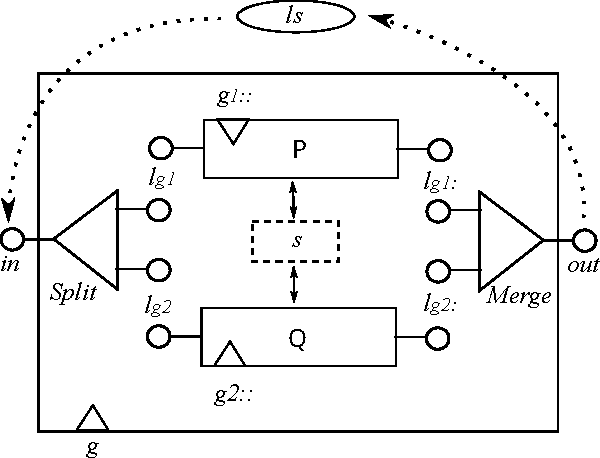
\includegraphics{images/par-comp-actual}

\subsection{seq-comp-actual}
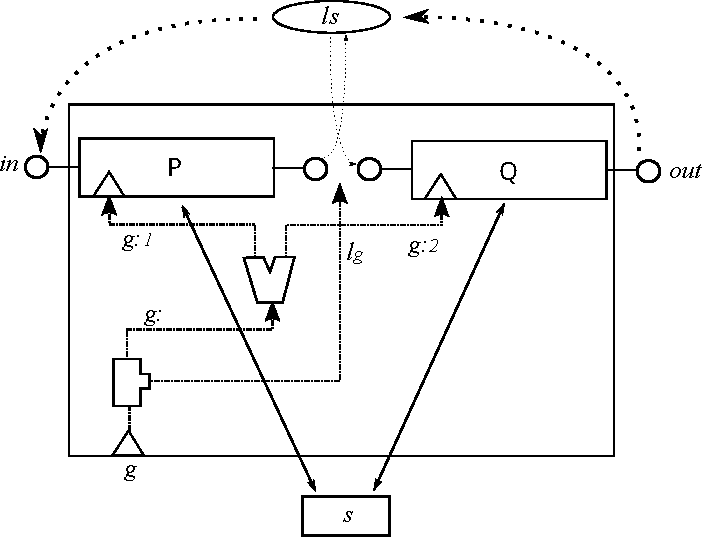
\includegraphics{images/seq-comp-actual}

\subsection{label-gen-example}
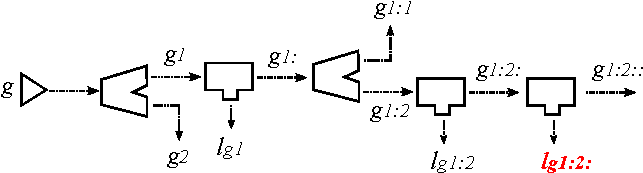
\includegraphics{images/label-gen-example}

\subsection{parallel-label-gen}
\includegraphics{images/parallel-label-gen}

\subsection{split-gen}
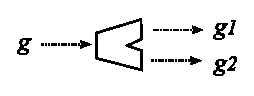
\includegraphics{images/split-gen}

\subsection{parallel-program}
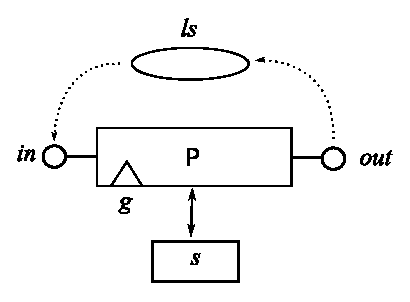
\includegraphics{images/parallel-program}

\subsection{seq-comp-idea}
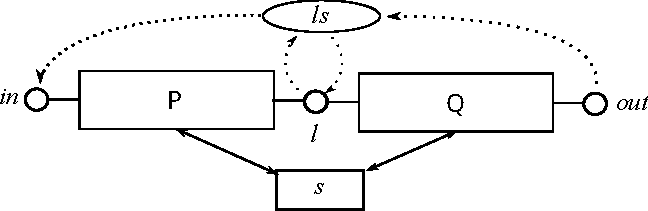
\includegraphics{images/seq-comp-idea}

\subsection{new-label}
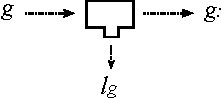
\includegraphics{images/new-label}


%\newpage
%\section{Math support for Views}\label{ha:mViews}

\subsection{The Big Plan}

We go for a new formulation
\RLEQNS{
   X(E|a|R|A) &\defs&
   ls(E) \land s' \in \sem a s \land ls' = (ls\setminus R)\cup A
\\ A(E|a|N) &\defs& X(E|a|E|N)
\\ \W(P) &\defs& \true * (\Skip \lor P)
\\       &=& \bigvee_{i \in \Nat} \Skip \seq P^i
\\ atm(a) &=& \W(A(in|a|out) \land [in|out])
\\ C &=& \W(actions(C) \land [in|out|g] \land I_C)
}
where $I_C$ is some more $C$-specific invariants.

\subsection{Set Inclusion/Membership}

An atomic action $A(E|a|N)$ is enabled if $E$ is contained
in the global label-set ($ls(E)$)
and results in $E$ being removed from that set, and new labels
$N$ being added ($ls'=(ls\setminus E)\cup N$).
We need a way to reason about containment in such an $ls'$
in terns of $E$ and $N$, and to compute sequential compositions
of such forms, which will take the more general form $X(E|a|R|A)$.

We find we get assertions of the form $(F(ls))(E)$,
asserting that $E$ is a subset of $F(ls)$ where $F$ is a set-function
composed of named/enumerated sets and standard set-operations.
We want to transform it into $ls(G) \land P$ where $G$ and $P$
do not involve $ls$.

We present the laws,
then the proofs
\RLEQNS{
   (ls \cup A)(S)      &=& ls(S\setminus A)
\\ (ls \setminus R)(S) &=& ls(S) \land S \cap R = \emptyset
\\ (ls \cap M)(S)      &=& ls(S) \land S \subseteq M
\\ ((ls \setminus R) \cup A)(S)
   &=& ls(S \setminus A) \land (S \setminus A) \cap R = \emptyset
\\ (((ls\setminus R_1) \cup A_1)\setminus R_2) \cup A_2
  &=& (ls \setminus (R_1 \cup R_2)) \cup ((A_1\setminus R_2) \cup A_2)
}

We do the proofs in ``classical'' set notation
\RLEQNS{
  && S \subseteq (ls \cup A)
\EQ{set definitions}
\\&& x \in S \implies x \in (ls \cup A)
\EQ{defn $\cup$}
\\&& x \in S \implies x \in ls \lor x \in A
\EQ{defn $\implies$}
\\&& x \notin S \lor x \in ls \lor x \in A
\EQ{rearrange}
\\&& x \notin S \lor x \in A \lor x \in ls
\EQ{De-Morgan, defn $\implies$}
\\&& (x \in S \land x \notin A) \implies x \in ls
\EQ{defn subset}
\\&& (S \setminus A) \subseteq ls
}

\RLEQNS{
  && S \subseteq (ls \setminus R)
\EQ{set definitions}
\\&& x \in S \implies x \in (ls \setminus R)
\EQ{set definition}
\\&& x \in S \implies x \in ls \land x \notin R
\EQ{defn $\implies$}
\\&& x \notin S \lor x \in ls \land x \notin R
\EQ{distribution}
\\&& (x \notin S \lor x \in ls)
     \land
     ( x \notin S \lor x \notin R)
\EQ{defn implies, de-morgan}
\\&& (x \in S \implies x \in ls)
     \land
     \lnot( x \in S \land x \in R)
\EQ{defn subset}
\\&&S \subseteq ls \land S \cap R = \emptyset
}

\RLEQNS{
  && S \subseteq (ls \cap M)
\EQ{set definitions}
\\&& x \in S \implies x \in ls \land x \in M
\EQ{defn $\implies$}
\\&& x \notin S \lor x \in ls \land x \in M
\EQ{distribution}
\\&& (x \notin S \lor x \in ls)
     \land
     (x \notin S \lor x \in M)
\EQ{defn $implies$}
\\&& (x \in S \implies x \in ls)
     \land
     (x \in S \implies x \in M)
\EQ{def subset}
\\&& S \subseteq ls \land S \subseteq M
}

\RLEQNS{
  && ((ls \setminus R) \cup A)(S)
\EQ{laws above}
\\&& (ls \setminus R)(S \setminus A)
\EQ{laws above}
\\&& ls(S \setminus A) \land (S \setminus A) \cap R = \emptyset
}

\RLEQNS{
  && x \in (ls\setminus R_1) \cup A_1
\EQ{defn $\cup$}
\\&& x \in (ls\setminus R_1) \lor x \in  A_1
\EQ{defn $\setminus$}
\\&& x \in ls \land x \notin R_1 \lor x \in  A_1
}

\RLEQNS{
  && x \in (((ls\setminus R_1) \cup A_1)\setminus R_2) \cup A_2
\EQ{above law}
\\&& x \in (ls\setminus R_1) \cup A_1) \land x \notin R_2 \lor x \in  A_2
\EQ{above law}
\\&& (x \in ls \land x \notin R_1 \lor x \in  A_1) \land x \notin R_2 \lor x \in  A_2
\EQ{distributivity}
\\&& (x \in ls \land x \notin R_1 \land x \notin R_2)
     \lor
     (x \in  A_1 \land x \notin R_2)
     \lor x \in  A_2
\EQ{de-Morgan, defn $\setminus$}
\\&& (x \in ls \land \lnot(x \in R_1 \lor x \in R_2))
     \lor
     x \in  A_1 \setminus R_2
     \lor x \in  A_2
\EQ{defn $\cup$, twice}
\\&& (x \in ls \land \lnot(x \in R_1 \cup R_2))
     \lor
     x \in  A_1 \setminus R_2 \cup  A_2
\EQ{tweak}
\\&& (x \in ls \land x \notin R_1 \cup R_2)
     \lor
     x \in  A_1 \setminus R_2 \cup  A_2
\EQ{definition of $\setminus$}
\\&& x \in (ls \setminus R_1 \cup R_2)
     \lor
     x \in  A_1 \setminus R_2 \cup  A_2
\EQ{definition of $cup$}
\\&& x \in (ls \setminus R_1 \cup R_2)
     \cup
     (A_1 \setminus R_2 \cup  A_2)
}

\subsection{Basic Actions}

We define a basic operation form that is closed
under sequential composition, modulo some `ground' side-conditions.
\RLEQNS{
   X(E|a|R|A)
   &\defs&
   ls(E) \land [a] \land ls' = (ls\setminus R) \cup A
}
Composing these requires us decouple the enabling labels
from those removed---they are the same for a basic action,
but differ as they are sequentially composed.

The general composition:
\RLEQNS{
  && X(E_1|a|R_1|A_1)\seq X(E_2|b|R_2|A_2)
\EQ{Defn $X$}
\\&& ls(E_1) \land [a] \land ls' = (ls\setminus R_1) \cup A_1
     \quad\seq\quad
     ls(E_2) \land [b] \land ls' = (ls\setminus R_2) \cup A_2
\EQ{Defn $\seq$}
\\&& \exists s_m,ls_m @
\\&& \quad ls(E_1) \land
           [a][s_m/s'] \land
           ls_m = (ls\setminus R_1) \cup A_1 \land {}
\\&& \quad ls_m(E_2) \land
           [b][s_m/s] \land
           ls' = (ls_m\setminus R_2) \cup A_2
\EQ{1-pt rule ($ls_m$), re-arrange}
\\&& \exists s_m @
\\&& \quad ls(E_1) \land
           ((ls\setminus R_1) \cup A_1)(E_2) \land {}
\\&& \quad [a][s_m/s'] \land
           [b][s_m/s] \land {}
\\&& \quad ls' = (((ls\setminus R_1) \cup A_1)\setminus R_2) \cup A_2
\EQ{shrink $s_m$ scope, use $ls(-)$ laws above}
\\&& ls(E_1) \land
     ls(E_2\setminus A_1) \land
     (E_2\setminus A_1) \cap R_1 = \emptyset \land {}
\\&& (\exists s_m @ [a][s_m/s'] \land [b][s_m/s]) \land {}
\\&& ls' = (((ls\setminus R_1) \cup A_1)\setminus R_2) \cup A_2
\EQ{defn $\seq$, prop of $ls(-)$, simplification from above}
\\&& ls(E_1 \cup (E_2\setminus A_1)) \land
     (E_2\setminus A_1) \cap R_1 = \emptyset \land {}
\\&& [a;b] \land {}
\\&& ls' = (ls \setminus R_1 \cup R_2)
           \cup
           (A_1 \setminus R_2 \cup  A_2)
\EQ{defn of $X$}
\\&& X(E_1 \cup (E_2\setminus A_1)
       |a\seq b
       |R_1 \cup R_2
       |A_1 \setminus R_2 \cup  A_2)
       \land (E_2\setminus A_1) \cap R_1 = \emptyset
}
Here the `ground' side-condition is
 $(E_2\setminus A_1) \cap R_1 = \emptyset$.

Composing a basic operation with itself:
\RLEQNS{
  && X(E|a|R|A) \seq X(E|a|R|A)
\EQ{by above}
\\&& X(E \cup (E\setminus A)
       |a\seq a
       |R \cup R
       |A \setminus R \cup  A)
       \land (E\setminus A) \cap R = \emptyset
\EQ{simpify}
\\&& X(E|a\seq a|R|A)
       \land (E\setminus A) \cap R = \emptyset
}

A basic action identifies $E$ and $R$:
\RLEQNS{
  && A(E|a|N) \defs X(E|a|E|N)
\\
\\&& A(E_1|a|N_1) \seq A(E_2|a|N_2)
\EQ{by defn}
\\&& A(E_1|a|E_1|N_1) \seq A(E_2|a|E_2|N_2)
\EQ{by calc above, with $R_i = E_i$}
\\&& X(E_1 \cup (E_2\setminus A_1)
       |a\seq b
       |E_1 \cup E_2
       |A_1 \setminus E_2 \cup  A_2)
       \land (E_2\setminus A_1) \cap E_1 = \emptyset
}
We cannot transform this into the form $A(-|a\seq b|-)$
unless it happens to be the case that
\\$E_1 \cup (E_2\setminus A_1)= E_1 \cup E_2$.
For an $A$ composed with itself:
\RLEQNS{
  && A(E|a|N) \seq A(E|a|N)
\EQ{defn $A$}
\\&& X(E|a|E|N) \seq X(E|a|E|N)
\EQ{calc above}
\\&& X(E|a\seq a|E|A)
       \land (E\setminus A) \cap E = \emptyset
}
We see that we get a $\false$ result unless we have $E \subseteq A$,
in which everything we remove is added back in, plus possibly some extra.
We get the following which is similar
\[
  X(E|a\seq a|\emptyset|A)
\]
This is a consequence of the following easy law:
\[
 (ls \setminus R) \cup A
 =
 (ls \setminus (R \setminus A)) \cup A
 =
 (ls \cup A) \setminus (R \setminus A)
\]

Following on, we can pre-compute mixed combinations:
\RLEQNS{
  && X(E_1|a|R_1|A_1) \seq A(E_2|b|N_2)
\EQ{defn $A$}
\\&& X(E_1|a|R_1|A_1) \seq X(E_2|b|E_2|N_2)
\EQ{law for $X$ above}
\\&& X(E_1 \cup (E_2 \setminus A_1)
      | a\seq b
      | R_1 \cup E_2
      | A_1 \setminus E_2 \cup N_2)
     \land
     (E_2 \setminus A_1) \cap R_1 = \emptyset
}
and flipped:
\RLEQNS{
  && A(E_1|a|N_1) \seq X(E_2|b|R_2|A_2)
\EQ{defn $A$}
\\&& X(E_1|a|E_1|N_1) \seq X(E_2|b|R_2|A_2)
\EQ{law for $X$ above}
\\&& X(E_1 \cup (E_2 \setminus N_1)
      | a\seq b
      | E_1 \cup R_2
      | N_1 \setminus R_2 \cup A_2)
     \land
     (E_2 \setminus N_1) \cap E_1 = \emptyset
}

\subsubsection{Laws of Actions}
Here we summarise the main results:
\RLEQNS{
  && X(E_1|a|R_1|A_1)\seq X(E_2|b|R_2|A_2)
\EQ{proof above}
\\&& X(E_1 \cup (E_2\setminus A_1)
       \mid a\seq b
       \mid R_1 \cup R_2
       \mid A_1 \setminus R_2 \cup  A_2)
\\&& {} \land (E_2\setminus A_1) \cap R_1 = \emptyset
\\
\\&& \\&& A(E_1|a|N_1) \seq A(E_2|a|N_2)
\EQ{proof above}
\\&& X(E_1 \cup (E_2\setminus N_1)
       \mid a\seq b
       \mid E_1 \cup E_2
       \mid N_1 \setminus E_2 \cup  N_2)
\\&& {} \land (E_2\setminus N_1) \cap E_1 = \emptyset
\\
\\&& A(E|a|N) \seq A(E|a|N)
\EQ{proof above}
\\&& X(E|a\seq a|E|N)   \land   (E\setminus N) \cap E = \emptyset
\EQ{simplify}
\\&& X(E|a\seq a|\emptyset|N)   \land   E \subseteq N
}



\newpage
\subsection{Working with the Invariant}

We have introduced the following notation:
\[
  [ L_1 | L_2 | \dots | L_n ]
\]
Its first intended meaning is to assert that
all the $L_i$ are mutually disjoint:
\RLEQNS{
   \forall i,j \in 1\dots n @ i \neq j \implies L_i \cap L_j = \emptyset
}
It also states that if any one of its members overlaps with $ls$,
then none of the others do (and similarly for $ls'$):
\RLEQNS{
  &&   \forall i,j \in 1\dots n @
        i \neq j \land L_i \cap ls \neq \emptyset
        \implies L_j \cap ls = \emptyset
\\&&   \forall i,j \in 1\dots n @
        i \neq j \land L_i \cap ls' \neq \emptyset
        \implies L_j \cap ls' = \emptyset
}

By \emph{design}, our labels and generator scheme
establishes the following (weakest) invariant:
\[ [in|out|g]\]
and for any generator expression $G$ we can split it into
four disjoint parts (also by design) to get
\[  [\ell_G|G_{:}|G_1|G_2] . \]
So we can always strengthen our invariant by splitting some $G$
in this way:
\RLEQNS{
  && [in|out|g]
\EQ{split $g$}
\\&& [in|out|\ell_g|\g:|\g1|\g2]
\EQ{split $\g:$}
\\&& [in|out|\ell_g| \ell_{g:}|\g{::}|\g{:1}|\g{:2}|\g1|\g2]
}
However, sometimes we don't want to do this.
The hope is that by requiring $[in|out|g]$ at each level,
that we get the right level of exclusivity vs. sharing of $ls$
by generated labels.

\subsubsection{Nested Invariants}


All of these comments above are true if the invariant is just about disjointness.
It is not true in general when we consider exclusivity.
For example in parallel execution it is perfectly reasonable to have both
$\ell_{g1}$ and $\ell_{g2:}$ (or $\ell_{g2}$) together in the label-set,
but not both $\ell_{g1}$ and $\ell_{g1:}$
or both $\ell_{g2}$ and $\ell_{g2:}$.

Notationally, we can represent this as follows:
$$
[in \mid [\ell_{g1}|\ell_{g1:}],[\ell_{g2}|\ell_{g2:}] \mid out].
$$
In effect this declares, at the top, that we have
$$
[in \mid \ell_{g1},\ell_{g1:},\ell_{g2},\ell_{g2:} \mid out]
$$
with finer grained details for the generated labels,
where a comma is a form of set union,
so we can have something from
either or both of $[\ell_{g1}|\ell_{g1:}]$ and $[\ell_{g2}|\ell_{g2:}]$
but within each of these we have mutual exclusion.

In effect we have a tree-like structure with ``$|$''-branches
and ``$,$``-branches, and labels as leaves.
We should be able to flatten cases where a subnode has the same branch type,
so
\RLEQNS{
   [L_1 \mid [L_{21}|L_{22}] \mid L_3]
   &=&
   [L_1|L_{21}|L_{22}|L_3]
\\ L_1 , ( L_{21}, L_{22})  , L_3
   &=&
   L_1,L_{21},L_{22},L_3
}



Invariants are based on the following general construct:
\RLEQNS{
   EXC_{i=1}^n A_i
   &\defs&
   \forall i,j \in 1\dots n @ i\neq j \land A_i \implies \lnot A_j
}
which we can also write as $EXC(A_1,\dots,A_n)$.
A quick calculation shows that
(using hardware logic notation for compactness):
\[
 EXC(A,B,C) = \B A ~ \B B  + \B A ~ \B C + \B B ~ \B C
\]
Do the following laws hold?
\RLEQNS{
   EXC(EXC(A,B),EXC(B,C)) &=& EXC(A,B,C)
\\ EXC(EXC(A,B),EXC(C,D)) &=& EXC(A,B,C,D)
}
No - the first lhs asserts that either $A$ and $B$ are exclusive,
or $B$ and $C$ are exclusive, but not both,
i.e. we have $EXC(A,B) \implies \lnot EXC(B,C)$.

How about:
\RLEQNS{
   EXC(A,B) \land EXC(B,C) &=& EXC(A,B,C)
\\ EXC(A,B) \land EXC(C,D) &=& EXC(A,B,C,D)
}
No, The first doesn't force the exclusivity of $A$ and $C$.

We need full information, so the following is required:
\RLEQNS{
   EXC(A,B) \land EXC(B,C) \land EXC(A,C) &=& EXC(A,B,C)
}
This works

Not sure interpreting $[L|M]$ or $EX(L,M)$ as predicates is helpful.
It might be better being viewed as a tree and defining a satisfaction relation
between it an a label-set.


\subsubsection{Using $A$ with invariants}

Noting that $[L_1|L_2|\dots]$ implies that if $ls(L_1)$ is true,
then $ls(L_2)$ is false:
\RLEQNS{
  && X(L_1|a|L_1,L_2|L_3) & [L_1|L_2|\dots]
\EQ{defn $X$}
\\&& ls(L_1) \land [a] \land ls'=(ls\setminus(L_1 \cup L_2)) \cup L_3
\EQ{no need to remove $L_2$ from $ls$ if it is not there}
\\&& ls(L_1) \land [a] \land ls'=(ls\setminus L_1) \cup L_3
\EQ{defn $X$}
\\&& X(L_1|a|L_1|L_3)
\EQ{defn $A$}
\\&& A(L_1|a|L_3)
}


Two actions meant to work together:
\RLEQNS{
  && A(L_1|a|L_2) \seq A(L_2|b|L_3) & [L_1|L_2|L_3]
\EQ{law $A^2$}
\\&& L_2\setminus L_2 \cap L_1 = \emptyset \land {}
\\&& X(    L_1 \cup L_2\setminus L_2
      \mid a\seq b
      \mid L_1 \cup L_2
      \mid L_2\setminus L_2 \cup L_3 )
\EQ{simplify}
\\&& X(    L_1
      \mid a\seq b
      \mid L_1 \cup L_2
      \mid  L_3 )
\EQ{prev law, given invariant}
\\&& X( L_1 |  a\seq b | L_1 | L_3 )
\EQ{defn $A$}
\\&& A( L_1 |  a\seq b | L_3 )
}

Two actions meant to be mutually exclusive (the hint being the invariant):
\RLEQNS{
  && A(L_1|a|L_2) \seq A(L_3|b|L_4) & [L_1|L_2|L_3|L_4]
\EQ{law $A^2$}
\\&& L_3\setminus L_2 \cap L_1 = \emptyset \and {}
\\&& X(    L_1 \cup L_3\setminus L_2
      \mid a\seq b
      \mid L_1 \cup L_3
      \mid L_2\setminus L_3 \cup L_4 )
\EQ{simplify, noting invariant}
\\&& X(    L_1 \cup L_3
      \mid a\seq b
      \mid L_1 \cup L_3
      \mid L_2 \cup L_4 )
\EQ{Falsifies $[L_1|L_3|\ldots]$}
\\&& \false
}
This law also works with invariant fragments
$[L_1|L_3|\dots]$ and $[L_2|L_4|\dots]$

\newpage
\subsection{Semantic Definitions}

\RLEQNS{
   X(E|a|R|A) &\defs&
   ls(E) \land s' \in \sem a s \land ls' = (ls\setminus R)\cup A
\\ A(E|a|N) &\defs& X(E|a|E|N)
\\ \W(P) &\defs& \true * (\Skip \lor P)
\\       &=& \bigvee_{i \in \Nat} \Skip \seq P^i
\\
\\ atm(a) &=& \W(A(in|a|out)) \land [in|out]
\\
\\ C \cseq D
   &\defs&
   \W( C[\ell_g,\g{:1}/out,g] \lor
       D[\ell_g,\g{:2}/in,g] ) \land [in|\ell_g|out]
\\
\\ C + D
   &\defs&
   \W(~ A(in|ii|\ell_{g1}) \lor
        A(in|ii|\ell_{g2}) \lor {}
\\&& ~~ C[g_{1:},\ell_{g1}/g,in] \lor
       D[g_{2:},\ell_{g2}/g,in]~ )
\\&& {}\land [in|\ell_{g1}|\ell_{g2}|out]
\\
\\ C \parallel D
   &\defs&
   \W(~
      A(in|ii|\ell_{g1},\ell_{g2}) \lor
      A(\ell_{g1:},\ell_{g2:}|ii|out) \lor {}
\\&& ~~
       C[g_{1::},\ell_{g1},\ell_{g1:}/g,in,out] \lor
       D[g_{2::},\ell_{g2},\ell_{g2:}/g,in,out] ~)
\\&& {} \land [in \mid [\ell_{g1}|\ell_{g1:}],[\ell_{g2}|\ell_{g2:}] \mid out]
\\
\\ C^*
   &\defs&
   \W(~ A(in|ii|out) \lor
       A(in|ii|\ell_g) \lor
       C[\g:,\ell_g,in/g,in,out] ~)
\\&& {} \land [in|\ell_g|out]
}

We note that $\W(P) \land I = \W(P \land I)$ for our invariants.

\newpage
\subsection{Semantic Calculations}

Semantic calculations will be based on the following form:
\[
  \W(P) = \Skip \lor \left(\bigvee_{i=1,\dots} P^i\right)
\]
So all we need to do is to compute $P^i$ for $i>1$
until we get either $\false$ or a prior result as outcome.
The semantics is the the disjunction of all of the results.

Note: where iteration is concerned, $P^i$ may never vanish
or converge, so the treatment there will be a little different.


\subsubsection{Atomic Action}

\[ atm(a) \defs \W(A(in|a|out)) \land [in|out] \]

\[ P = A(in|a|out) \qquad I = [in|out] \]

\RLEQNS{
  && P^2
\EQ{expand $P$}
\\&& A(in|a|out) \seq A(in|a|out)
\EQ{$A^2$ law}
\\&& X(in|a\seq a|\emptyset|out) \land in \subseteq out
\EQ{$I$ implies $in$, $out$ are disjoint}
\\&& \false
}

So, we can declare that:
\RLEQNS{
  && atm(a)
\EQ{calculations above}
\\&& (~\Skip \lor A(in|a|out)~) \land [in|out]
}

\newpage
\subsubsection{Sequential Composition}

\[
  C \cseq D
   \defs
   \W( C[\ell_g,\g{:1}/out,g] \lor
       D[\ell_g,\g{:2}/in,g] ) \land [in|\ell_g|out]
\]

\[ P =  atm(a)[\ell_g,\g{:1}/out,g] \lor
       atm(b)[\ell_g,\g{:2}/in,g]\qquad I = [in|\ell_g|out] \]

\RLEQNS{
  && P
\EQ{expand $P$}
\\&& atm(a)[\ell_g,\g{:1}/out,g]
     \lor
     atm(b)[\ell_g,\g{:2}/in,g]
\EQ{expand $atm$s}
\\&& ((\Skip \lor A(in|a|out)) \land [in|out])[\ell_g,\g{:1}/out,g]
     \lor {}
\\&& ((\Skip \lor A(in|b|out)) \land [in|out])[\ell_g,\g{:2}/in,g]
\EQ{substitution}
\\&& (\Skip \lor A(in|a|\ell_g)) \land [in|\ell_g]
     \lor {}
\\&& (\Skip \lor A(\ell_g|b|out) \land [\ell_g|out]
\EQ{$I$ subsumes both $atm$ invariants}
\\&& \Skip \lor A(in|a|\ell_g)
     \lor
     \Skip \lor A(\ell_g|b|out)
\EQ{tidy-up}
\\&& \Skip \lor A(in|a|\ell_g) \lor A(\ell_g|b|out)
}

We note that
\[
 \Skip \lor (\Skip \lor Q) \lor (\Skip \lor Q)^2
 \lor (\Skip \lor Q)^3 \lor \dots
\]
reduces to
\[
 \Skip \lor Q \lor Q^2 \lor Q^3 \lor \dots
\]

So we proceed with $Q$
\[
  Q = A(in|a|\ell_g) \lor A(\ell_g|b|out)
  \qquad
  I = [in|\ell_g|out]
\]

\RLEQNS{
  && Q^2
\EQ{expand $Q$}
\\&& (A(in|a|\ell_g) \lor A(\ell_g|b|out))
     \seq
     (A(in|a|\ell_g) \lor A(\ell_g|b|out))
\EQ{distribute}
\\&&     A(in|a|\ell_g)
         \seq
         A(in|a|\ell_g)
\\&\lor& A(in|a|\ell_g)
         \seq
         A(\ell_g|b|out)
\\&\lor& A(\ell_g|b|out)
         \seq
         A(in|a|\ell_g)
\\&\lor& A(\ell_g|b|out)
         \seq
         A(\ell_g|b|out)
\EQ{prop $A^2$}
\\&&     in\setminus \ell_g \cap in = \emptyset \land \dots
\\&\lor& \ell_g\setminus \ell_g \cap in = \emptyset
         \land X( in\cup\ell_g\setminus \ell_g
                \mid a \seq b
                \mid in,\ell_g
                \mid \ell_g\setminus\ell_g\cup out )
\\&\lor& in\setminus out \cap \ell_g = \emptyset
         \land X(\ell_g\cup in \setminus out
                \mid b\seq a
                \mid \ell_g,in
                \mid out\setminus in \cup\ell_g )
\\&\lor& \ell_g\setminus out \cap \ell_g = \emptyset \land \dots
\EQ{simplify}
\\&&     X( in
                \mid a \seq b
                \mid in,\ell_g
                \mid out )
\\&\lor& X( \ell_g,in
                \mid b\seq a
                \mid \ell_g,in
                \mid out, \ell_g )
\EQ{2nd disjunct falsifies $[in|\ell_g|out]$}
\\&&     X( in |a \seq b | in,\ell_g | out )
\EQ{$[in|\ell_g|out]$ implies there will be no $\ell_g$ to remove}
\\&&     X( in |a \seq b | in | out )
\EQ{defn $A$}
\\&&     A( in |a \seq b | out )
}


\RLEQNS{
  && Q^3
\EQ{expand $Q\seq Q^2$}
\\&& (A(in|a|\ell_g) \lor A(\ell_g|b|out))
     \seq  X( in |a \seq b | in,\ell_g | out )
\EQ{distribute, expand $A$}
\\&&     X( in | a | in | \ell_g)
         \seq
         X( in |a \seq b | in,\ell_g | out )
\\&\lor& X( \ell_g | b | \ell_g | out)
         \seq
         X( in |a \seq b | in,\ell_g | out )
\EQ{prop $X^2$}
\\&&     in \setminus \ell_g \cap in = \emptyset \land\dots
\\&\lor& in\setminus out \cap \ell_g = \emptyset \land {}
         X( \ell_g \cup in \setminus out
          | b\seq a\seq b
          | in,\ell_g
          | out\setminus\setof{in,\ell_g} \cup out )
\EQ{simplify}
\\&& X( \ell_g,in
      | b\seq a\seq b
      | in,\ell_g
      | out )
\EQ{Falsifies $[in|\ell_g|out]$}
\\&& \false
}
So we see that $Q^n$ vanishes for $n\geq 3$.

So we have
\RLEQNS{
  && atm(a)\seq atm(b)
\EQ{$Q$ expansion}
\\&& \Skip \lor Q \lor Q^2 \lor Q^3 \lor \dots
\EQ{$Q^n = \false$ for $n \geq 3$}
\\&& \Skip \lor Q \lor Q^2
\EQ{expand $Q^i$}
\\&&     \Skip
\\&\lor& A(in|a|\ell_g) \lor A(\ell_g|b|out)
\\&\lor& A( in |a \seq b | out )
}


\newpage
\subsubsection{Choice}


\RLEQNS{
   C + D
   &\defs&
   \W(~ A(in|ii|\ell_{g1}) \lor
        A(in|ii|\ell_{g2}) \lor {}
\\&& \quad~~ C[g_{1:},\ell_{g1}/g,in] \lor
       D[g_{2:},\ell_{g2}/g,in]~ )
\\&& {}\land [in|\ell_{g1}|\ell_{g2}|out]
}

\RLEQNS{
   P &=& A(in|ii|\ell_{g1}) \lor
         A(in|ii|\ell_{g2}) \lor {}
\\   & & atm(a)[g_{1:},\ell_{g1}/g,in] \lor
         atm(b)[g_{2:},\ell_{g2}/g,in]
\\
\\ I &=& [in|\ell_{g1}|\ell_{g2}|out]
}

\RLEQNS{
  && P
\EQ{expand $P$}
\\&& A(in|ii|\ell_{g1}) \lor
     A(in|ii|\ell_{g2}) \lor {}
\\&& atm(a)[g_{1:},\ell_{g1}/g,in] \lor
     atm(b)[g_{2:},\ell_{g2}/g,in]
\EQ{expand $atm$}
\\&& A(in|ii|\ell_{g1}) \lor
     A(in|ii|\ell_{g2}) \lor {}
\\&& ((\Skip \lor A(in|a|out)) \land [in|out])
     [g_{1:},\ell_{g1}/g,in] \lor {}
\\&& ((\Skip \lor A(in|b|out)) \land [in|out])
     [g_{2:},\ell_{g2}/g,in]
\EQ{substitute}
\\&& A(in|ii|\ell_{g1}) \lor
     A(in|ii|\ell_{g2}) \lor {}
\\&& (\Skip \lor A(\ell_{g1}|a|out)) \land [\ell_{g1}|out] \lor
     (\Skip \lor A(\ell_{g2}|b|out)) \land [\ell_{g2}|out]
\EQ{sub-invariants subsumed by $I$}
\\&& A(in|ii|\ell_{g1}) \lor
     A(in|ii|\ell_{g2}) \lor {}
\\&& \Skip \lor A(\ell_{g1}|a|out) \lor
     \Skip \lor A(\ell_{g2}|b|out)
\EQ{re-arrange, simplify}
\\&& \Skip \lor A(in|ii|\ell_{g1}) \lor
     A(in|ii|\ell_{g2}) \lor
     A(\ell_{g1}|a|out) \lor
     A(\ell_{g2}|b|out)
\EQ{$Q$ again}
\\&& \Skip \lor Q
}

\RLEQNS{
  && Q^2
\EQ{defn $Q$}
\\&& (~ A(in|ii|\ell_{g1}) \lor
     A(in|ii|\ell_{g2}) \lor
     A(\ell_{g1}|a|out) \lor
     A(\ell_{g2}|b|out)~) \seq{}
\\&& (~ A(in|ii|\ell_{g1}) \lor
     A(in|ii|\ell_{g2}) \lor
     A(\ell_{g1}|a|out) \lor
     A(\ell_{g2}|b|out)~)
\EQ{distribute,
    noting condition $(E_2\setminus N_1)\cap E_1=\emptyset $}
\\&    & A(in|ii|\ell_{g1}) \seq A(in|ii|\ell_{g1}) \quad \mbox{--- fail}
\\&\lor& A(in|ii|\ell_{g1}) \seq A(in|ii|\ell_{g2}) \quad \mbox{--- fail}
\\&\lor& A(in|ii|\ell_{g1}) \seq A(\ell_{g1}|a|out) \quad \mbox{--- ok}
\\&\lor& A(in|ii|\ell_{g1}) \seq A(\ell_{g2}|b|out) \quad \mbox{--- ok}
\\&\lor& A(in|ii|\ell_{g2}) \seq A(in|ii|\ell_{g1}) \quad \mbox{--- fail}
\\&\lor& A(in|ii|\ell_{g2}) \seq A(in|ii|\ell_{g2}) \quad \mbox{--- fail}
\\&\lor& A(in|ii|\ell_{g2}) \seq A(\ell_{g1}|a|out) \quad \mbox{--- ok}
\\&\lor& A(in|ii|\ell_{g2}) \seq A(\ell_{g2}|b|out) \quad \mbox{--- ok}
\\&\lor& A(\ell_{g1}|a|out) \seq A(in|ii|\ell_{g1}) \quad \mbox{--- ok}
\\&\lor& A(\ell_{g1}|a|out) \seq A(in|ii|\ell_{g2}) \quad \mbox{--- ok}
\\&\lor& A(\ell_{g1}|a|out) \seq A(\ell_{g1}|a|out) \quad \mbox{--- fail}
\\&\lor& A(\ell_{g1}|a|out) \seq A(\ell_{g2}|b|out) \quad \mbox{--- ok}
\\&\lor& A(\ell_{g2}|b|out) \seq A(in|ii|\ell_{g1}) \quad \mbox{--- ok}
\\&\lor& A(\ell_{g2}|b|out) \seq A(in|ii|\ell_{g2}) \quad \mbox{--- ok}
\\&\lor& A(\ell_{g2}|b|out) \seq A(\ell_{g1}|a|out) \quad \mbox{--- ok}
\\&\lor& A(\ell_{g2}|b|out) \seq A(\ell_{g2}|b|out) \quad \mbox{--- fail}
\EQ{drop fails, apply $A^2$ work together law w.r.t $I$}
\\&    & A(in|ii\seq a|out)
\\&\lor& A(in|ii|\ell_{g1}) \seq A(\ell_{g2}|b|out)
\\&\lor& A(in|ii|\ell_{g2}) \seq A(\ell_{g1}|a|out)
\\&\lor& A(in|ii \seq b|out)
\\&\lor& A(\ell_{g1}|a|out) \seq A(in|ii|\ell_{g1})
\\&\lor& A(\ell_{g1}|a|out) \seq A(in|ii|\ell_{g2})
\\&\lor& A(\ell_{g1}|a|out) \seq A(\ell_{g2}|b|out)
\\&\lor& A(\ell_{g2}|b|out) \seq A(in|ii|\ell_{g1})
\\&\lor& A(\ell_{g2}|b|out) \seq A(in|ii|\ell_{g2})
\\&\lor& A(\ell_{g2}|b|out) \seq A(\ell_{g1}|a|out)
\EQ{apply $A^2$ mutually-exclusive law w.r.t. $I$}
\\&    & A(in|ii\seq a|out)
\\&\lor& A(in|ii\seq b|out)
\EQ{$ii$ is unit for $\seq$ over $s$, $s'$}
\\&& A(in|a|out) \lor A(in|b|out)
}

\RLEQNS{
  && Q^3
\EQ{split as $Q^2 \seq Q$}
\\&& (A(in|a|out) \lor A(in|b|out)) \seq {}
\\&& (~ A(in|ii|\ell_{g1}) \lor
     A(in|ii|\ell_{g2}) \lor
     A(\ell_{g1}|a|out) \lor
     A(\ell_{g2}|b|out)~)
\EQ{distribute}
\\&    & A(in|a|out) \seq A(in|ii|\ell_{g1}) \quad \mbox{--- $A^2$ cond fail}
\\&\lor& A(in|a|out) \seq A(in|ii|\ell_{g2}) \quad \mbox{--- $A^2$ cond fail}
\\&\lor& A(in|a|out) \seq A(\ell_{g1}|a|out) \quad \mbox{--- mut-exc fail}
\\&\lor& A(in|a|out) \seq A(\ell_{g2}|b|out) \quad \mbox{--- mut-exc fail}
\\&\lor& A(in|b|out) \seq A(in|ii|\ell_{g1}) \quad \mbox{--- $A^2$ cond fail}
\\&\lor& A(in|b|out) \seq A(in|ii|\ell_{g2}) \quad \mbox{--- $A^2$ cond fail}
\\&\lor& A(in|b|out) \seq A(\ell_{g1}|a|out) \quad \mbox{--- mut-exc fail}
\\&\lor& A(in|b|out) \seq A(\ell_{g2}|b|out) \quad \mbox{--- mut-exc fail}
\EQ{all gone!}
\\&& \false
}
So, we go as far as $Q^2$:

\RLEQNS{
  && atm(a)+atm(b)
\EQ{$Q$ expansion}
\\&& \Skip \lor Q \lor Q^2
\EQ{expand $Q^i$}
\\&& \Skip \lor A(in|ii|\ell_{g1}) \lor A(in|ii|\ell_{g2}) \lor {}
\\&& A(\ell_{g1}|a|out) \lor A(\ell_{g2}|b|out) \lor{}
\\&& A(in|a|out) \lor A(in|b|out)
}

\newpage
\subsubsection{Parallel Composition}


\RLEQNS{
   C \parallel D
   &\defs&
   \W(~
      A(in|ii|\ell_{g1},\ell_{g2}) \lor
      A(\ell_{g1:},\ell_{g2:}|ii|out) \lor {}
\\&& ~~
       C[g_{1::},\ell_{g1},\ell_{g1:}/g,in,out] \lor
       D[g_{2::},\ell_{g2},\ell_{g2:}/g,in,out] ~)
\\&& {} \land [in|\ell_{g1},\ell_{g2}|\ell_{g1:},\ell_{g2:}|out]
}

\RLEQNS{
   P &=& A(in|ii|\ell_{g1},\ell_{g2}) \lor
         A(\ell_{g1:},\ell_{g2:}|ii|out) \lor {}
\\   & & atm(a)[g_{1::},\ell_{g1},\ell_{g1:}/g,in,out] \lor
         atm(b)[g_{2::},\ell_{g2},\ell_{g2:}/g,in,out]
\\
\\ I &=& [in\mid[\ell_{g1}|\ell_{g1:}],[\ell_{g2}|\ell_{g2:}]\mid out]
\\ && \mbox{Note the new complicated invariant!}
}

\RLEQNS{
  && P
\EQ{expand $P$}
\\&& A(in|ii|\ell_{g1},\ell_{g2}) \lor
     A(\ell_{g1:},\ell_{g2:}|ii|out) \lor {}
\\&& atm(a)[g_{1::},\ell_{g1},\ell_{g1:}/g,in,out] \lor
     atm(b)[g_{2::},\ell_{g2},\ell_{g2:}/g,in,out]
\EQ{expand $atm$}
\\&& A(in|ii|\ell_{g1},\ell_{g2}) \lor
     A(\ell_{g1:},\ell_{g2:}|ii|out) \lor {}
\\&& ((\Skip \lor A(in|a|out)) \land [in|out])
     [g_{1::},\ell_{g1},\ell_{g1:}/g,in,out] \lor {}
\\&& ((\Skip \lor A(in|b|out)) \land [in|out])
     [g_{2::},\ell_{g2},\ell_{g2:}/g,in,out]
\EQ{substitution}
\\&& A(in|ii|\ell_{g1},\ell_{g2}) \lor
     A(\ell_{g1:},\ell_{g2:}|ii|out) \lor {}
\\&& (\Skip \lor A(\ell_{g1}|a|\ell_{g1:})) \land [\ell_{g1}|\ell_{g1:}] \lor {}
\\&& (\Skip \lor A(\ell_{g2}|b|\ell_{g2:})) \land [\ell_{g2}|\ell_{g2:}]
\EQ{atomic invariants subsumed by $I$}
\\&& A(in|ii|\ell_{g1},\ell_{g2}) \lor
     A(\ell_{g1:},\ell_{g2:}|ii|out) \lor {}
\\&& \Skip \lor A(\ell_{g1}|a|\ell_{g1:}) \lor \Skip \lor A(\ell_{g2}|b|\ell_{g2:})
\EQ{re-arrange, simplify}
\\&& \Skip \lor
     A(in|ii|\ell_{g1},\ell_{g2}) \lor
     A(\ell_{g1:},\ell_{g2:}|ii|out) \lor
     A(\ell_{g1}|a|\ell_{g1:}) \lor
     A(\ell_{g2}|b|\ell_{g2:})
\EQ{$Q$ again}
\\&& \Skip \lor Q
}

\RLEQNS{
  && Q^2
\EQ{expand $Q$}
\\&& (~ A(in|ii|\ell_{g1},\ell_{g2}) \lor
        A(\ell_{g1:},\ell_{g2:}|ii|out) \lor {}
\\&& ~~ A(\ell_{g1}|a|\ell_{g1:}) \lor
        A(\ell_{g2}|b|\ell_{g2:}) ~) \seq {}
\\&& (~ A(in|ii|\ell_{g1},\ell_{g2}) \lor
        A(\ell_{g1:},\ell_{g2:}|ii|out) \lor {}
\\&& ~~ A(\ell_{g1}|a|\ell_{g1:}) \lor
        A(\ell_{g2}|b|\ell_{g2:}) ~)
\EQ{distr., assess w.r.t $A^2$, $[in|\ell_{g1},\ell_{g2}|\ell_{g1:},\ell_{g2:}|out]$}
\\&\lor& A(in|ii|\ell_{g1},\ell_{g2})
    \seq A(in|ii|\ell_{g1},\ell_{g2})    & fail
\\&\lor& A(in|ii|\ell_{g1},\ell_{g2})
    \seq A(\ell_{g1:},\ell_{g2:}|ii|out) & fail
\\&\lor& A(in|ii|\ell_{g1},\ell_{g2})
    \seq A(\ell_{g1}|a|\ell_{g1:})       & ok
\\&\lor& A(in|ii|\ell_{g1},\ell_{g2})
    \seq A(\ell_{g2}|b|\ell_{g2:})       & ok
\\&\lor& A(\ell_{g1:},\ell_{g2:}|ii|out)
    \seq A(in|ii|\ell_{g1},\ell_{g2})    & fail
\\&\lor& A(\ell_{g1:},\ell_{g2:}|ii|out)
    \seq A(\ell_{g1:},\ell_{g2:}|ii|out) & fail
\\&\lor& A(\ell_{g1:},\ell_{g2:}|ii|out)
    \seq A(\ell_{g1}|a|\ell_{g1:})       & fail
\\&\lor& A(\ell_{g1:},\ell_{g2:}|ii|out)
    \seq A(\ell_{g2}|b|\ell_{g2:})       & fail
\\&\lor& A(\ell_{g1}|a|\ell_{g1:})
    \seq A(in|ii|\ell_{g1},\ell_{g2})    & fail
\\&\lor& A(\ell_{g1}|a|\ell_{g1:})
    \seq A(\ell_{g1:},\ell_{g2:}|ii|out) & ok
\\&\lor& A(\ell_{g1}|a|\ell_{g1:})
    \seq A(\ell_{g1}|a|\ell_{g1:})       & fail
\\&\lor& A(\ell_{g1}|a|\ell_{g1:})
    \seq A(\ell_{g2}|b|\ell_{g2:})       & ok
\\&\lor& A(\ell_{g2}|b|\ell_{g2:})
    \seq A(in|ii|\ell_{g1},\ell_{g2})    & fail
\\&\lor& A(\ell_{g2}|b|\ell_{g2:})
    \seq A(\ell_{g1:},\ell_{g2:}|ii|out) & ok
\\&\lor& A(\ell_{g2}|b|\ell_{g2:})
    \seq A(\ell_{g1}|a|\ell_{g1:})       & ok
\\&\lor& A(\ell_{g2}|b|\ell_{g2:})
    \seq A(\ell_{g2}|b|\ell_{g2:})       & fail
\EQ{drop fails}
\\&\lor& A(in|ii|\ell_{g1},\ell_{g2})
    \seq A(\ell_{g1}|a|\ell_{g1:})       & ok
\\&\lor& A(in|ii|\ell_{g1},\ell_{g2})
    \seq A(\ell_{g2}|b|\ell_{g2:})       & ok
\\&\lor& A(\ell_{g1}|a|\ell_{g1:})
    \seq A(\ell_{g1:},\ell_{g2:}|ii|out) & ok
\\&\lor& A(\ell_{g1}|a|\ell_{g1:})
    \seq A(\ell_{g2}|b|\ell_{g2:})       & ok
\\&\lor& A(\ell_{g2}|b|\ell_{g2:})
    \seq A(\ell_{g1:},\ell_{g2:}|ii|out) & ok
\\&\lor& A(\ell_{g2}|b|\ell_{g2:})
    \seq A(\ell_{g1}|a|\ell_{g1:})       & ok
\EQ{law $A^2$}
\\&& \mbox{the calculator might be a good idea at this point!}
}
We will need to go to $Q^4$, and show that $Q^5$ is $\false$.

\newpage
\subsubsection{Iteration}

A quick pen'n'paper calculation for $atm(a)^*$ yields:
\[\begin{array}{rcccc}
   Q   &=& in\arr{} out & in\arr{}\ell_g & in\arr{a} in
\\ Q^2 &=& in \arr{a} in & \ell_g \arr{a} out & \ell_g \arr{a} \ell_g
\\ Q^3   &=& in\arr{a} out & in\arr{a}\ell_g & in\arr{aa} in
\\ Q^4 &=& in \arr{aa} in & \ell_g \arr{aa} out & \ell_g \arr{aa} \ell_g
\\ Q^5   &=& in\arr{aa} out & in\arr{aa}\ell_g & in\arr{aaa} in
\\ Q^6 &=& in \arr{aaa} in & \ell_g \arr{aaa} out & \ell_g \arr{aaa} \ell_g
\end{array}\]


\newpage
\subsection{Semantic Results}

\RLEQNS{
   atm(a)
   &=&
   (~\Skip \lor A(in|a|out)~) \land [in|out]
\\ atm(a)\seq atm(b)
   &=& (~\Skip \lor
         A(in|a|\ell_g) \lor
         A(\ell_g|b|out) \lor
         A(in|a \seq b| out) ~)
\\&& {} \land [in|\ell_g|out]
\\ atm(a)+atm(b)
   &=& (~\Skip \lor A(in|ii|\ell_{g1}) \lor A(in|ii|\ell_{g2}) \lor {}
\\&& A(\ell_{g1}|a|out) \lor A(\ell_{g2}|b|out) \lor{}
\\&& A(in|a|out) \lor A(in|b|out)~)
\\&& {} \land [in|\ell_{g1}|\ell_{g2}|out]
}


Better formatting(?): 1st line is invariant,
other lines are the disjuncts (poss. several on one line), with $\Skip$ ommitted

\RLEQNS{
   atm(a)
   &=& [in|out]
\\ & & A(in|a|out)
\\
\\ atm(a)\seq atm(b)
   &=& [in|\ell_g|out]
\\ & & A(in|a|\ell_g) \quad A(\ell_g|b|out)
\\ & & A(in|a \seq b|out)
\\
\\ atm(a)+atm(b)
   &=& [in|\ell_{g1}|\ell_{g2}|out]
\\ & & A(in|ii|\ell_{g1}) \quad A(in|ii|\ell_{g2})
\\ & & A(\ell_{g1}|a|out) \quad A(\ell_{g2}|b|out)
\\ & & A(in|a|out) \quad A(in|b|out)
}


%\section{Math support for Views}\label{ha:mViews}

\subsection{The Big Plan}

We go for a new formulation
\RLEQNS{
   X(E|a|R|A) &\defs&
   ls(E) \land s' \in \sem a s \land ls' = (ls\setminus R)\cup A
\\ A(E|a|N) &\defs& X(E|a|E|N)
\\ \W(P) &\defs& \true * (\Skip \lor P)
\\       &=& \bigvee_{i \in \Nat} \Skip \seq P^i
\\ atm(a) &=& \W(A(in|a|out) \land [in|out])
\\ C &=& \W(actions(C) \land [in|out|g] \land I_C)
}
where $I_C$ is some more $C$-specific invariants.

\subsection{Set Inclusion/Membership}

An atomic action $A(E|a|N)$ is enabled if $E$ is contained
in the global label-set ($ls(E)$)
and results in $E$ being removed from that set, and new labels
$N$ being added ($ls'=(ls\setminus E)\cup N$).
We need a way to reason about containment in such an $ls'$
in terns of $E$ and $N$, and to compute sequential compositions
of such forms, which will take the more general form $X(E|a|R|A)$.

We find we get assertions of the form $(F(ls))(E)$,
asserting that $E$ is a subset of $F(ls)$ where $F$ is a set-function
composed of named/enumerated sets and standard set-operations.
We want to transform it into $ls(G) \land P$ where $G$ and $P$
do not involve $ls$.

We present the laws,
then the proofs
\RLEQNS{
   (ls \cup A)(S)      &=& ls(S\setminus A)
\\ (ls \setminus R)(S) &=& ls(S) \land S \cap R = \emptyset
\\ (ls \cap M)(S)      &=& ls(S) \land S \subseteq M
\\ ((ls \setminus R) \cup A)(S)
   &=& ls(S \setminus A) \land (S \setminus A) \cap R = \emptyset
\\ (((ls\setminus R_1) \cup A_1)\setminus R_2) \cup A_2
  &=& (ls \setminus (R_1 \cup R_2)) \cup ((A_1\setminus R_2) \cup A_2)
}

We do the proofs in ``classical'' set notation
\RLEQNS{
  && S \subseteq (ls \cup A)
\EQ{set definitions}
\\&& x \in S \implies x \in (ls \cup A)
\EQ{defn $\cup$}
\\&& x \in S \implies x \in ls \lor x \in A
\EQ{defn $\implies$}
\\&& x \notin S \lor x \in ls \lor x \in A
\EQ{rearrange}
\\&& x \notin S \lor x \in A \lor x \in ls
\EQ{De-Morgan, defn $\implies$}
\\&& (x \in S \land x \notin A) \implies x \in ls
\EQ{defn subset}
\\&& (S \setminus A) \subseteq ls
}

\RLEQNS{
  && S \subseteq (ls \setminus R)
\EQ{set definitions}
\\&& x \in S \implies x \in (ls \setminus R)
\EQ{set definition}
\\&& x \in S \implies x \in ls \land x \notin R
\EQ{defn $\implies$}
\\&& x \notin S \lor x \in ls \land x \notin R
\EQ{distribution}
\\&& (x \notin S \lor x \in ls)
     \land
     ( x \notin S \lor x \notin R)
\EQ{defn implies, de-morgan}
\\&& (x \in S \implies x \in ls)
     \land
     \lnot( x \in S \land x \in R)
\EQ{defn subset}
\\&&S \subseteq ls \land S \cap R = \emptyset
}

\RLEQNS{
  && S \subseteq (ls \cap M)
\EQ{set definitions}
\\&& x \in S \implies x \in ls \land x \in M
\EQ{defn $\implies$}
\\&& x \notin S \lor x \in ls \land x \in M
\EQ{distribution}
\\&& (x \notin S \lor x \in ls)
     \land
     (x \notin S \lor x \in M)
\EQ{defn $implies$}
\\&& (x \in S \implies x \in ls)
     \land
     (x \in S \implies x \in M)
\EQ{def subset}
\\&& S \subseteq ls \land S \subseteq M
}

\RLEQNS{
  && ((ls \setminus R) \cup A)(S)
\EQ{laws above}
\\&& (ls \setminus R)(S \setminus A)
\EQ{laws above}
\\&& ls(S \setminus A) \land (S \setminus A) \cap R = \emptyset
}

\RLEQNS{
  && x \in (ls\setminus R_1) \cup A_1
\EQ{defn $\cup$}
\\&& x \in (ls\setminus R_1) \lor x \in  A_1
\EQ{defn $\setminus$}
\\&& x \in ls \land x \notin R_1 \lor x \in  A_1
}

\RLEQNS{
  && x \in (((ls\setminus R_1) \cup A_1)\setminus R_2) \cup A_2
\EQ{above law}
\\&& x \in (ls\setminus R_1) \cup A_1) \land x \notin R_2 \lor x \in  A_2
\EQ{above law}
\\&& (x \in ls \land x \notin R_1 \lor x \in  A_1) \land x \notin R_2 \lor x \in  A_2
\EQ{distributivity}
\\&& (x \in ls \land x \notin R_1 \land x \notin R_2)
     \lor
     (x \in  A_1 \land x \notin R_2)
     \lor x \in  A_2
\EQ{de-Morgan, defn $\setminus$}
\\&& (x \in ls \land \lnot(x \in R_1 \lor x \in R_2))
     \lor
     x \in  A_1 \setminus R_2
     \lor x \in  A_2
\EQ{defn $\cup$, twice}
\\&& (x \in ls \land \lnot(x \in R_1 \cup R_2))
     \lor
     x \in  A_1 \setminus R_2 \cup  A_2
\EQ{tweak}
\\&& (x \in ls \land x \notin R_1 \cup R_2)
     \lor
     x \in  A_1 \setminus R_2 \cup  A_2
\EQ{definition of $\setminus$}
\\&& x \in (ls \setminus R_1 \cup R_2)
     \lor
     x \in  A_1 \setminus R_2 \cup  A_2
\EQ{definition of $cup$}
\\&& x \in (ls \setminus R_1 \cup R_2)
     \cup
     (A_1 \setminus R_2 \cup  A_2)
}

\subsection{Basic Actions}

We define a basic operation form that is closed
under sequential composition, modulo some `ground' side-conditions.
\RLEQNS{
   X(E|a|R|A)
   &\defs&
   ls(E) \land [a] \land ls' = (ls\setminus R) \cup A
}
Composing these requires us decouple the enabling labels
from those removed---they are the same for a basic action,
but differ as they are sequentially composed.

The general composition:
\RLEQNS{
  && X(E_1|a|R_1|A_1)\seq X(E_2|b|R_2|A_2)
\EQ{Defn $X$}
\\&& ls(E_1) \land [a] \land ls' = (ls\setminus R_1) \cup A_1
     \quad\seq\quad
     ls(E_2) \land [b] \land ls' = (ls\setminus R_2) \cup A_2
\EQ{Defn $\seq$}
\\&& \exists s_m,ls_m @
\\&& \quad ls(E_1) \land
           [a][s_m/s'] \land
           ls_m = (ls\setminus R_1) \cup A_1 \land {}
\\&& \quad ls_m(E_2) \land
           [b][s_m/s] \land
           ls' = (ls_m\setminus R_2) \cup A_2
\EQ{1-pt rule ($ls_m$), re-arrange}
\\&& \exists s_m @
\\&& \quad ls(E_1) \land
           ((ls\setminus R_1) \cup A_1)(E_2) \land {}
\\&& \quad [a][s_m/s'] \land
           [b][s_m/s] \land {}
\\&& \quad ls' = (((ls\setminus R_1) \cup A_1)\setminus R_2) \cup A_2
\EQ{shrink $s_m$ scope, use $ls(-)$ laws above}
\\&& ls(E_1) \land
     ls(E_2\setminus A_1) \land
     (E_2\setminus A_1) \cap R_1 = \emptyset \land {}
\\&& (\exists s_m @ [a][s_m/s'] \land [b][s_m/s]) \land {}
\\&& ls' = (((ls\setminus R_1) \cup A_1)\setminus R_2) \cup A_2
\EQ{defn $\seq$, prop of $ls(-)$, simplification from above}
\\&& ls(E_1 \cup (E_2\setminus A_1)) \land
     (E_2\setminus A_1) \cap R_1 = \emptyset \land {}
\\&& [a;b] \land {}
\\&& ls' = (ls \setminus R_1 \cup R_2)
           \cup
           (A_1 \setminus R_2 \cup  A_2)
\EQ{defn of $X$}
\\&& X(E_1 \cup (E_2\setminus A_1)
       |a\seq b
       |R_1 \cup R_2
       |A_1 \setminus R_2 \cup  A_2)
       \land (E_2\setminus A_1) \cap R_1 = \emptyset
}
Here the `ground' side-condition is
 $(E_2\setminus A_1) \cap R_1 = \emptyset$.

Composing a basic operation with itself:
\RLEQNS{
  && X(E|a|R|A) \seq X(E|a|R|A)
\EQ{by above}
\\&& X(E \cup (E\setminus A)
       |a\seq a
       |R \cup R
       |A \setminus R \cup  A)
       \land (E\setminus A) \cap R = \emptyset
\EQ{simpify}
\\&& X(E|a\seq a|R|A)
       \land (E\setminus A) \cap R = \emptyset
}

A basic action identifies $E$ and $R$:
\RLEQNS{
  && A(E|a|N) \defs X(E|a|E|N)
\\
\\&& A(E_1|a|N_1) \seq A(E_2|a|N_2)
\EQ{by defn}
\\&& A(E_1|a|E_1|N_1) \seq A(E_2|a|E_2|N_2)
\EQ{by calc above, with $R_i = E_i$}
\\&& X(E_1 \cup (E_2\setminus A_1)
       |a\seq b
       |E_1 \cup E_2
       |A_1 \setminus E_2 \cup  A_2)
       \land (E_2\setminus A_1) \cap E_1 = \emptyset
}
We cannot transform this into the form $A(-|a\seq b|-)$
unless it happens to be the case that
\\$E_1 \cup (E_2\setminus A_1)= E_1 \cup E_2$.
For an $A$ composed with itself:
\RLEQNS{
  && A(E|a|N) \seq A(E|a|N)
\EQ{defn $A$}
\\&& X(E|a|E|N) \seq X(E|a|E|N)
\EQ{calc above}
\\&& X(E|a\seq a|E|A)
       \land (E\setminus A) \cap E = \emptyset
}
We see that we get a $\false$ result unless we have $E \subseteq A$,
in which everything we remove is added back in, plus possibly some extra.
We get the following which is similar
\[
  X(E|a\seq a|\emptyset|A)
\]
This is a consequence of the following easy law:
\[
 (ls \setminus R) \cup A
 =
 (ls \setminus (R \setminus A)) \cup A
 =
 (ls \cup A) \setminus (R \setminus A)
\]

Following on, we can pre-compute mixed combinations:
\RLEQNS{
  && X(E_1|a|R_1|A_1) \seq A(E_2|b|N_2)
\EQ{defn $A$}
\\&& X(E_1|a|R_1|A_1) \seq X(E_2|b|E_2|N_2)
\EQ{law for $X$ above}
\\&& X(E_1 \cup (E_2 \setminus A_1)
      | a\seq b
      | R_1 \cup E_2
      | A_1 \setminus E_2 \cup N_2)
     \land
     (E_2 \setminus A_1) \cap R_1 = \emptyset
}
and flipped:
\RLEQNS{
  && A(E_1|a|N_1) \seq X(E_2|b|R_2|A_2)
\EQ{defn $A$}
\\&& X(E_1|a|E_1|N_1) \seq X(E_2|b|R_2|A_2)
\EQ{law for $X$ above}
\\&& X(E_1 \cup (E_2 \setminus N_1)
      | a\seq b
      | E_1 \cup R_2
      | N_1 \setminus R_2 \cup A_2)
     \land
     (E_2 \setminus N_1) \cap E_1 = \emptyset
}

\subsubsection{Laws of Actions}
Here we summarise the main results:
\RLEQNS{
  && X(E_1|a|R_1|A_1)\seq X(E_2|b|R_2|A_2)
\EQ{proof above}
\\&& X(E_1 \cup (E_2\setminus A_1)
       \mid a\seq b
       \mid R_1 \cup R_2
       \mid A_1 \setminus R_2 \cup  A_2)
\\&& {} \land (E_2\setminus A_1) \cap R_1 = \emptyset
\\
\\&& \\&& A(E_1|a|N_1) \seq A(E_2|a|N_2)
\EQ{proof above}
\\&& X(E_1 \cup (E_2\setminus N_1)
       \mid a\seq b
       \mid E_1 \cup E_2
       \mid N_1 \setminus E_2 \cup  N_2)
\\&& {} \land (E_2\setminus N_1) \cap E_1 = \emptyset
\\
\\&& A(E|a|N) \seq A(E|a|N)
\EQ{proof above}
\\&& X(E|a\seq a|E|N)   \land   (E\setminus N) \cap E = \emptyset
\EQ{simplify}
\\&& X(E|a\seq a|\emptyset|N)   \land   E \subseteq N
}



\newpage
\subsection{Working with the Invariant}

We have introduced the following notation:
\[
  [ L_1 | L_2 | \dots | L_n ]
\]
Its first intended meaning is to assert that
all the $L_i$ are mutually disjoint:
\RLEQNS{
   \forall i,j \in 1\dots n @ i \neq j \implies L_i \cap L_j = \emptyset
}
It also states that if any one of its members overlaps with $ls$,
then none of the others do (and similarly for $ls'$):
\RLEQNS{
  &&   \forall i,j \in 1\dots n @
        i \neq j \land L_i \cap ls \neq \emptyset
        \implies L_j \cap ls = \emptyset
\\&&   \forall i,j \in 1\dots n @
        i \neq j \land L_i \cap ls' \neq \emptyset
        \implies L_j \cap ls' = \emptyset
}

By \emph{design}, our labels and generator scheme
establishes the following (weakest) invariant:
\[ [in|out|g]\]
and for any generator expression $G$ we can split it into
four disjoint parts (also by design) to get
\[  [\ell_G|G_{:}|G_1|G_2] . \]
So we can always strengthen our invariant by splitting some $G$
in this way:
\RLEQNS{
  && [in|out|g]
\EQ{split $g$}
\\&& [in|out|\ell_g|\g:|\g1|\g2]
\EQ{split $\g:$}
\\&& [in|out|\ell_g| \ell_{g:}|\g{::}|\g{:1}|\g{:2}|\g1|\g2]
}
However, sometimes we don't want to do this.
The hope is that by requiring $[in|out|g]$ at each level,
that we get the right level of exclusivity vs. sharing of $ls$
by generated labels.

\subsubsection{Nested Invariants}


All of these comments above are true if the invariant is just about disjointness.
It is not true in general when we consider exclusivity.
For example in parallel execution it is perfectly reasonable to have both
$\ell_{g1}$ and $\ell_{g2:}$ (or $\ell_{g2}$) together in the label-set,
but not both $\ell_{g1}$ and $\ell_{g1:}$
or both $\ell_{g2}$ and $\ell_{g2:}$.

Notationally, we can represent this as follows:
$$
[in \mid [\ell_{g1}|\ell_{g1:}],[\ell_{g2}|\ell_{g2:}] \mid out].
$$
In effect this declares, at the top, that we have
$$
[in \mid \ell_{g1},\ell_{g1:},\ell_{g2},\ell_{g2:} \mid out]
$$
with finer grained details for the generated labels,
where a comma is a form of set union,
so we can have something from
either or both of $[\ell_{g1}|\ell_{g1:}]$ and $[\ell_{g2}|\ell_{g2:}]$
but within each of these we have mutual exclusion.

In effect we have a tree-like structure with ``$|$''-branches
and ``$,$``-branches, and labels as leaves.
We should be able to flatten cases where a subnode has the same branch type,
so
\RLEQNS{
   [L_1 \mid [L_{21}|L_{22}] \mid L_3]
   &=&
   [L_1|L_{21}|L_{22}|L_3]
\\ L_1 , ( L_{21}, L_{22})  , L_3
   &=&
   L_1,L_{21},L_{22},L_3
}



Invariants are based on the following general construct:
\RLEQNS{
   EXC_{i=1}^n A_i
   &\defs&
   \forall i,j \in 1\dots n @ i\neq j \land A_i \implies \lnot A_j
}
which we can also write as $EXC(A_1,\dots,A_n)$.
A quick calculation shows that
(using hardware logic notation for compactness):
\[
 EXC(A,B,C) = \B A ~ \B B  + \B A ~ \B C + \B B ~ \B C
\]
Do the following laws hold?
\RLEQNS{
   EXC(EXC(A,B),EXC(B,C)) &=& EXC(A,B,C)
\\ EXC(EXC(A,B),EXC(C,D)) &=& EXC(A,B,C,D)
}
No - the first lhs asserts that either $A$ and $B$ are exclusive,
or $B$ and $C$ are exclusive, but not both,
i.e. we have $EXC(A,B) \implies \lnot EXC(B,C)$.

How about:
\RLEQNS{
   EXC(A,B) \land EXC(B,C) &=& EXC(A,B,C)
\\ EXC(A,B) \land EXC(C,D) &=& EXC(A,B,C,D)
}
No, The first doesn't force the exclusivity of $A$ and $C$.

We need full information, so the following is required:
\RLEQNS{
   EXC(A,B) \land EXC(B,C) \land EXC(A,C) &=& EXC(A,B,C)
}
This works

Not sure interpreting $[L|M]$ or $EX(L,M)$ as predicates is helpful.
It might be better being viewed as a tree and defining a satisfaction relation
between it an a label-set.


\subsubsection{Using $A$ with invariants}

Noting that $[L_1|L_2|\dots]$ implies that if $ls(L_1)$ is true,
then $ls(L_2)$ is false:
\RLEQNS{
  && X(L_1|a|L_1,L_2|L_3) & [L_1|L_2|\dots]
\EQ{defn $X$}
\\&& ls(L_1) \land [a] \land ls'=(ls\setminus(L_1 \cup L_2)) \cup L_3
\EQ{no need to remove $L_2$ from $ls$ if it is not there}
\\&& ls(L_1) \land [a] \land ls'=(ls\setminus L_1) \cup L_3
\EQ{defn $X$}
\\&& X(L_1|a|L_1|L_3)
\EQ{defn $A$}
\\&& A(L_1|a|L_3)
}


Two actions meant to work together:
\RLEQNS{
  && A(L_1|a|L_2) \seq A(L_2|b|L_3) & [L_1|L_2|L_3]
\EQ{law $A^2$}
\\&& L_2\setminus L_2 \cap L_1 = \emptyset \land {}
\\&& X(    L_1 \cup L_2\setminus L_2
      \mid a\seq b
      \mid L_1 \cup L_2
      \mid L_2\setminus L_2 \cup L_3 )
\EQ{simplify}
\\&& X(    L_1
      \mid a\seq b
      \mid L_1 \cup L_2
      \mid  L_3 )
\EQ{prev law, given invariant}
\\&& X( L_1 |  a\seq b | L_1 | L_3 )
\EQ{defn $A$}
\\&& A( L_1 |  a\seq b | L_3 )
}

Two actions meant to be mutually exclusive (the hint being the invariant):
\RLEQNS{
  && A(L_1|a|L_2) \seq A(L_3|b|L_4) & [L_1|L_2|L_3|L_4]
\EQ{law $A^2$}
\\&& L_3\setminus L_2 \cap L_1 = \emptyset \and {}
\\&& X(    L_1 \cup L_3\setminus L_2
      \mid a\seq b
      \mid L_1 \cup L_3
      \mid L_2\setminus L_3 \cup L_4 )
\EQ{simplify, noting invariant}
\\&& X(    L_1 \cup L_3
      \mid a\seq b
      \mid L_1 \cup L_3
      \mid L_2 \cup L_4 )
\EQ{Falsifies $[L_1|L_3|\ldots]$}
\\&& \false
}
This law also works with invariant fragments
$[L_1|L_3|\dots]$ and $[L_2|L_4|\dots]$

\newpage
\subsection{Semantic Definitions}

\RLEQNS{
   X(E|a|R|A) &\defs&
   ls(E) \land s' \in \sem a s \land ls' = (ls\setminus R)\cup A
\\ A(E|a|N) &\defs& X(E|a|E|N)
\\ \W(P) &\defs& \true * (\Skip \lor P)
\\       &=& \bigvee_{i \in \Nat} \Skip \seq P^i
\\
\\ atm(a) &=& \W(A(in|a|out)) \land [in|out]
\\
\\ C \cseq D
   &\defs&
   \W( C[\ell_g,\g{:1}/out,g] \lor
       D[\ell_g,\g{:2}/in,g] ) \land [in|\ell_g|out]
\\
\\ C + D
   &\defs&
   \W(~ A(in|ii|\ell_{g1}) \lor
        A(in|ii|\ell_{g2}) \lor {}
\\&& ~~ C[g_{1:},\ell_{g1}/g,in] \lor
       D[g_{2:},\ell_{g2}/g,in]~ )
\\&& {}\land [in|\ell_{g1}|\ell_{g2}|out]
\\
\\ C \parallel D
   &\defs&
   \W(~
      A(in|ii|\ell_{g1},\ell_{g2}) \lor
      A(\ell_{g1:},\ell_{g2:}|ii|out) \lor {}
\\&& ~~
       C[g_{1::},\ell_{g1},\ell_{g1:}/g,in,out] \lor
       D[g_{2::},\ell_{g2},\ell_{g2:}/g,in,out] ~)
\\&& {} \land [in \mid [\ell_{g1}|\ell_{g1:}],[\ell_{g2}|\ell_{g2:}] \mid out]
\\
\\ C^*
   &\defs&
   \W(~ A(in|ii|out) \lor
       A(in|ii|\ell_g) \lor
       C[\g:,\ell_g,in/g,in,out] ~)
\\&& {} \land [in|\ell_g|out]
}

We note that $\W(P) \land I = \W(P \land I)$ for our invariants.

\newpage
\subsection{Semantic Calculations}

Semantic calculations will be based on the following form:
\[
  \W(P) = \Skip \lor \left(\bigvee_{i=1,\dots} P^i\right)
\]
So all we need to do is to compute $P^i$ for $i>1$
until we get either $\false$ or a prior result as outcome.
The semantics is the the disjunction of all of the results.

Note: where iteration is concerned, $P^i$ may never vanish
or converge, so the treatment there will be a little different.


\subsubsection{Atomic Action}

\[ atm(a) \defs \W(A(in|a|out)) \land [in|out] \]

\[ P = A(in|a|out) \qquad I = [in|out] \]

\RLEQNS{
  && P^2
\EQ{expand $P$}
\\&& A(in|a|out) \seq A(in|a|out)
\EQ{$A^2$ law}
\\&& X(in|a\seq a|\emptyset|out) \land in \subseteq out
\EQ{$I$ implies $in$, $out$ are disjoint}
\\&& \false
}

So, we can declare that:
\RLEQNS{
  && atm(a)
\EQ{calculations above}
\\&& (~\Skip \lor A(in|a|out)~) \land [in|out]
}

\newpage
\subsubsection{Sequential Composition}

\[
  C \cseq D
   \defs
   \W( C[\ell_g,\g{:1}/out,g] \lor
       D[\ell_g,\g{:2}/in,g] ) \land [in|\ell_g|out]
\]

\[ P =  atm(a)[\ell_g,\g{:1}/out,g] \lor
       atm(b)[\ell_g,\g{:2}/in,g]\qquad I = [in|\ell_g|out] \]

\RLEQNS{
  && P
\EQ{expand $P$}
\\&& atm(a)[\ell_g,\g{:1}/out,g]
     \lor
     atm(b)[\ell_g,\g{:2}/in,g]
\EQ{expand $atm$s}
\\&& ((\Skip \lor A(in|a|out)) \land [in|out])[\ell_g,\g{:1}/out,g]
     \lor {}
\\&& ((\Skip \lor A(in|b|out)) \land [in|out])[\ell_g,\g{:2}/in,g]
\EQ{substitution}
\\&& (\Skip \lor A(in|a|\ell_g)) \land [in|\ell_g]
     \lor {}
\\&& (\Skip \lor A(\ell_g|b|out) \land [\ell_g|out]
\EQ{$I$ subsumes both $atm$ invariants}
\\&& \Skip \lor A(in|a|\ell_g)
     \lor
     \Skip \lor A(\ell_g|b|out)
\EQ{tidy-up}
\\&& \Skip \lor A(in|a|\ell_g) \lor A(\ell_g|b|out)
}

We note that
\[
 \Skip \lor (\Skip \lor Q) \lor (\Skip \lor Q)^2
 \lor (\Skip \lor Q)^3 \lor \dots
\]
reduces to
\[
 \Skip \lor Q \lor Q^2 \lor Q^3 \lor \dots
\]

So we proceed with $Q$
\[
  Q = A(in|a|\ell_g) \lor A(\ell_g|b|out)
  \qquad
  I = [in|\ell_g|out]
\]

\RLEQNS{
  && Q^2
\EQ{expand $Q$}
\\&& (A(in|a|\ell_g) \lor A(\ell_g|b|out))
     \seq
     (A(in|a|\ell_g) \lor A(\ell_g|b|out))
\EQ{distribute}
\\&&     A(in|a|\ell_g)
         \seq
         A(in|a|\ell_g)
\\&\lor& A(in|a|\ell_g)
         \seq
         A(\ell_g|b|out)
\\&\lor& A(\ell_g|b|out)
         \seq
         A(in|a|\ell_g)
\\&\lor& A(\ell_g|b|out)
         \seq
         A(\ell_g|b|out)
\EQ{prop $A^2$}
\\&&     in\setminus \ell_g \cap in = \emptyset \land \dots
\\&\lor& \ell_g\setminus \ell_g \cap in = \emptyset
         \land X( in\cup\ell_g\setminus \ell_g
                \mid a \seq b
                \mid in,\ell_g
                \mid \ell_g\setminus\ell_g\cup out )
\\&\lor& in\setminus out \cap \ell_g = \emptyset
         \land X(\ell_g\cup in \setminus out
                \mid b\seq a
                \mid \ell_g,in
                \mid out\setminus in \cup\ell_g )
\\&\lor& \ell_g\setminus out \cap \ell_g = \emptyset \land \dots
\EQ{simplify}
\\&&     X( in
                \mid a \seq b
                \mid in,\ell_g
                \mid out )
\\&\lor& X( \ell_g,in
                \mid b\seq a
                \mid \ell_g,in
                \mid out, \ell_g )
\EQ{2nd disjunct falsifies $[in|\ell_g|out]$}
\\&&     X( in |a \seq b | in,\ell_g | out )
\EQ{$[in|\ell_g|out]$ implies there will be no $\ell_g$ to remove}
\\&&     X( in |a \seq b | in | out )
\EQ{defn $A$}
\\&&     A( in |a \seq b | out )
}


\RLEQNS{
  && Q^3
\EQ{expand $Q\seq Q^2$}
\\&& (A(in|a|\ell_g) \lor A(\ell_g|b|out))
     \seq  X( in |a \seq b | in,\ell_g | out )
\EQ{distribute, expand $A$}
\\&&     X( in | a | in | \ell_g)
         \seq
         X( in |a \seq b | in,\ell_g | out )
\\&\lor& X( \ell_g | b | \ell_g | out)
         \seq
         X( in |a \seq b | in,\ell_g | out )
\EQ{prop $X^2$}
\\&&     in \setminus \ell_g \cap in = \emptyset \land\dots
\\&\lor& in\setminus out \cap \ell_g = \emptyset \land {}
         X( \ell_g \cup in \setminus out
          | b\seq a\seq b
          | in,\ell_g
          | out\setminus\setof{in,\ell_g} \cup out )
\EQ{simplify}
\\&& X( \ell_g,in
      | b\seq a\seq b
      | in,\ell_g
      | out )
\EQ{Falsifies $[in|\ell_g|out]$}
\\&& \false
}
So we see that $Q^n$ vanishes for $n\geq 3$.

So we have
\RLEQNS{
  && atm(a)\seq atm(b)
\EQ{$Q$ expansion}
\\&& \Skip \lor Q \lor Q^2 \lor Q^3 \lor \dots
\EQ{$Q^n = \false$ for $n \geq 3$}
\\&& \Skip \lor Q \lor Q^2
\EQ{expand $Q^i$}
\\&&     \Skip
\\&\lor& A(in|a|\ell_g) \lor A(\ell_g|b|out)
\\&\lor& A( in |a \seq b | out )
}


\newpage
\subsubsection{Choice}


\RLEQNS{
   C + D
   &\defs&
   \W(~ A(in|ii|\ell_{g1}) \lor
        A(in|ii|\ell_{g2}) \lor {}
\\&& \quad~~ C[g_{1:},\ell_{g1}/g,in] \lor
       D[g_{2:},\ell_{g2}/g,in]~ )
\\&& {}\land [in|\ell_{g1}|\ell_{g2}|out]
}

\RLEQNS{
   P &=& A(in|ii|\ell_{g1}) \lor
         A(in|ii|\ell_{g2}) \lor {}
\\   & & atm(a)[g_{1:},\ell_{g1}/g,in] \lor
         atm(b)[g_{2:},\ell_{g2}/g,in]
\\
\\ I &=& [in|\ell_{g1}|\ell_{g2}|out]
}

\RLEQNS{
  && P
\EQ{expand $P$}
\\&& A(in|ii|\ell_{g1}) \lor
     A(in|ii|\ell_{g2}) \lor {}
\\&& atm(a)[g_{1:},\ell_{g1}/g,in] \lor
     atm(b)[g_{2:},\ell_{g2}/g,in]
\EQ{expand $atm$}
\\&& A(in|ii|\ell_{g1}) \lor
     A(in|ii|\ell_{g2}) \lor {}
\\&& ((\Skip \lor A(in|a|out)) \land [in|out])
     [g_{1:},\ell_{g1}/g,in] \lor {}
\\&& ((\Skip \lor A(in|b|out)) \land [in|out])
     [g_{2:},\ell_{g2}/g,in]
\EQ{substitute}
\\&& A(in|ii|\ell_{g1}) \lor
     A(in|ii|\ell_{g2}) \lor {}
\\&& (\Skip \lor A(\ell_{g1}|a|out)) \land [\ell_{g1}|out] \lor
     (\Skip \lor A(\ell_{g2}|b|out)) \land [\ell_{g2}|out]
\EQ{sub-invariants subsumed by $I$}
\\&& A(in|ii|\ell_{g1}) \lor
     A(in|ii|\ell_{g2}) \lor {}
\\&& \Skip \lor A(\ell_{g1}|a|out) \lor
     \Skip \lor A(\ell_{g2}|b|out)
\EQ{re-arrange, simplify}
\\&& \Skip \lor A(in|ii|\ell_{g1}) \lor
     A(in|ii|\ell_{g2}) \lor
     A(\ell_{g1}|a|out) \lor
     A(\ell_{g2}|b|out)
\EQ{$Q$ again}
\\&& \Skip \lor Q
}

\RLEQNS{
  && Q^2
\EQ{defn $Q$}
\\&& (~ A(in|ii|\ell_{g1}) \lor
     A(in|ii|\ell_{g2}) \lor
     A(\ell_{g1}|a|out) \lor
     A(\ell_{g2}|b|out)~) \seq{}
\\&& (~ A(in|ii|\ell_{g1}) \lor
     A(in|ii|\ell_{g2}) \lor
     A(\ell_{g1}|a|out) \lor
     A(\ell_{g2}|b|out)~)
\EQ{distribute,
    noting condition $(E_2\setminus N_1)\cap E_1=\emptyset $}
\\&    & A(in|ii|\ell_{g1}) \seq A(in|ii|\ell_{g1}) \quad \mbox{--- fail}
\\&\lor& A(in|ii|\ell_{g1}) \seq A(in|ii|\ell_{g2}) \quad \mbox{--- fail}
\\&\lor& A(in|ii|\ell_{g1}) \seq A(\ell_{g1}|a|out) \quad \mbox{--- ok}
\\&\lor& A(in|ii|\ell_{g1}) \seq A(\ell_{g2}|b|out) \quad \mbox{--- ok}
\\&\lor& A(in|ii|\ell_{g2}) \seq A(in|ii|\ell_{g1}) \quad \mbox{--- fail}
\\&\lor& A(in|ii|\ell_{g2}) \seq A(in|ii|\ell_{g2}) \quad \mbox{--- fail}
\\&\lor& A(in|ii|\ell_{g2}) \seq A(\ell_{g1}|a|out) \quad \mbox{--- ok}
\\&\lor& A(in|ii|\ell_{g2}) \seq A(\ell_{g2}|b|out) \quad \mbox{--- ok}
\\&\lor& A(\ell_{g1}|a|out) \seq A(in|ii|\ell_{g1}) \quad \mbox{--- ok}
\\&\lor& A(\ell_{g1}|a|out) \seq A(in|ii|\ell_{g2}) \quad \mbox{--- ok}
\\&\lor& A(\ell_{g1}|a|out) \seq A(\ell_{g1}|a|out) \quad \mbox{--- fail}
\\&\lor& A(\ell_{g1}|a|out) \seq A(\ell_{g2}|b|out) \quad \mbox{--- ok}
\\&\lor& A(\ell_{g2}|b|out) \seq A(in|ii|\ell_{g1}) \quad \mbox{--- ok}
\\&\lor& A(\ell_{g2}|b|out) \seq A(in|ii|\ell_{g2}) \quad \mbox{--- ok}
\\&\lor& A(\ell_{g2}|b|out) \seq A(\ell_{g1}|a|out) \quad \mbox{--- ok}
\\&\lor& A(\ell_{g2}|b|out) \seq A(\ell_{g2}|b|out) \quad \mbox{--- fail}
\EQ{drop fails, apply $A^2$ work together law w.r.t $I$}
\\&    & A(in|ii\seq a|out)
\\&\lor& A(in|ii|\ell_{g1}) \seq A(\ell_{g2}|b|out)
\\&\lor& A(in|ii|\ell_{g2}) \seq A(\ell_{g1}|a|out)
\\&\lor& A(in|ii \seq b|out)
\\&\lor& A(\ell_{g1}|a|out) \seq A(in|ii|\ell_{g1})
\\&\lor& A(\ell_{g1}|a|out) \seq A(in|ii|\ell_{g2})
\\&\lor& A(\ell_{g1}|a|out) \seq A(\ell_{g2}|b|out)
\\&\lor& A(\ell_{g2}|b|out) \seq A(in|ii|\ell_{g1})
\\&\lor& A(\ell_{g2}|b|out) \seq A(in|ii|\ell_{g2})
\\&\lor& A(\ell_{g2}|b|out) \seq A(\ell_{g1}|a|out)
\EQ{apply $A^2$ mutually-exclusive law w.r.t. $I$}
\\&    & A(in|ii\seq a|out)
\\&\lor& A(in|ii\seq b|out)
\EQ{$ii$ is unit for $\seq$ over $s$, $s'$}
\\&& A(in|a|out) \lor A(in|b|out)
}

\RLEQNS{
  && Q^3
\EQ{split as $Q^2 \seq Q$}
\\&& (A(in|a|out) \lor A(in|b|out)) \seq {}
\\&& (~ A(in|ii|\ell_{g1}) \lor
     A(in|ii|\ell_{g2}) \lor
     A(\ell_{g1}|a|out) \lor
     A(\ell_{g2}|b|out)~)
\EQ{distribute}
\\&    & A(in|a|out) \seq A(in|ii|\ell_{g1}) \quad \mbox{--- $A^2$ cond fail}
\\&\lor& A(in|a|out) \seq A(in|ii|\ell_{g2}) \quad \mbox{--- $A^2$ cond fail}
\\&\lor& A(in|a|out) \seq A(\ell_{g1}|a|out) \quad \mbox{--- mut-exc fail}
\\&\lor& A(in|a|out) \seq A(\ell_{g2}|b|out) \quad \mbox{--- mut-exc fail}
\\&\lor& A(in|b|out) \seq A(in|ii|\ell_{g1}) \quad \mbox{--- $A^2$ cond fail}
\\&\lor& A(in|b|out) \seq A(in|ii|\ell_{g2}) \quad \mbox{--- $A^2$ cond fail}
\\&\lor& A(in|b|out) \seq A(\ell_{g1}|a|out) \quad \mbox{--- mut-exc fail}
\\&\lor& A(in|b|out) \seq A(\ell_{g2}|b|out) \quad \mbox{--- mut-exc fail}
\EQ{all gone!}
\\&& \false
}
So, we go as far as $Q^2$:

\RLEQNS{
  && atm(a)+atm(b)
\EQ{$Q$ expansion}
\\&& \Skip \lor Q \lor Q^2
\EQ{expand $Q^i$}
\\&& \Skip \lor A(in|ii|\ell_{g1}) \lor A(in|ii|\ell_{g2}) \lor {}
\\&& A(\ell_{g1}|a|out) \lor A(\ell_{g2}|b|out) \lor{}
\\&& A(in|a|out) \lor A(in|b|out)
}

\newpage
\subsubsection{Parallel Composition}


\RLEQNS{
   C \parallel D
   &\defs&
   \W(~
      A(in|ii|\ell_{g1},\ell_{g2}) \lor
      A(\ell_{g1:},\ell_{g2:}|ii|out) \lor {}
\\&& ~~
       C[g_{1::},\ell_{g1},\ell_{g1:}/g,in,out] \lor
       D[g_{2::},\ell_{g2},\ell_{g2:}/g,in,out] ~)
\\&& {} \land [in|\ell_{g1},\ell_{g2}|\ell_{g1:},\ell_{g2:}|out]
}

\RLEQNS{
   P &=& A(in|ii|\ell_{g1},\ell_{g2}) \lor
         A(\ell_{g1:},\ell_{g2:}|ii|out) \lor {}
\\   & & atm(a)[g_{1::},\ell_{g1},\ell_{g1:}/g,in,out] \lor
         atm(b)[g_{2::},\ell_{g2},\ell_{g2:}/g,in,out]
\\
\\ I &=& [in\mid[\ell_{g1}|\ell_{g1:}],[\ell_{g2}|\ell_{g2:}]\mid out]
\\ && \mbox{Note the new complicated invariant!}
}

\RLEQNS{
  && P
\EQ{expand $P$}
\\&& A(in|ii|\ell_{g1},\ell_{g2}) \lor
     A(\ell_{g1:},\ell_{g2:}|ii|out) \lor {}
\\&& atm(a)[g_{1::},\ell_{g1},\ell_{g1:}/g,in,out] \lor
     atm(b)[g_{2::},\ell_{g2},\ell_{g2:}/g,in,out]
\EQ{expand $atm$}
\\&& A(in|ii|\ell_{g1},\ell_{g2}) \lor
     A(\ell_{g1:},\ell_{g2:}|ii|out) \lor {}
\\&& ((\Skip \lor A(in|a|out)) \land [in|out])
     [g_{1::},\ell_{g1},\ell_{g1:}/g,in,out] \lor {}
\\&& ((\Skip \lor A(in|b|out)) \land [in|out])
     [g_{2::},\ell_{g2},\ell_{g2:}/g,in,out]
\EQ{substitution}
\\&& A(in|ii|\ell_{g1},\ell_{g2}) \lor
     A(\ell_{g1:},\ell_{g2:}|ii|out) \lor {}
\\&& (\Skip \lor A(\ell_{g1}|a|\ell_{g1:})) \land [\ell_{g1}|\ell_{g1:}] \lor {}
\\&& (\Skip \lor A(\ell_{g2}|b|\ell_{g2:})) \land [\ell_{g2}|\ell_{g2:}]
\EQ{atomic invariants subsumed by $I$}
\\&& A(in|ii|\ell_{g1},\ell_{g2}) \lor
     A(\ell_{g1:},\ell_{g2:}|ii|out) \lor {}
\\&& \Skip \lor A(\ell_{g1}|a|\ell_{g1:}) \lor \Skip \lor A(\ell_{g2}|b|\ell_{g2:})
\EQ{re-arrange, simplify}
\\&& \Skip \lor
     A(in|ii|\ell_{g1},\ell_{g2}) \lor
     A(\ell_{g1:},\ell_{g2:}|ii|out) \lor
     A(\ell_{g1}|a|\ell_{g1:}) \lor
     A(\ell_{g2}|b|\ell_{g2:})
\EQ{$Q$ again}
\\&& \Skip \lor Q
}

\RLEQNS{
  && Q^2
\EQ{expand $Q$}
\\&& (~ A(in|ii|\ell_{g1},\ell_{g2}) \lor
        A(\ell_{g1:},\ell_{g2:}|ii|out) \lor {}
\\&& ~~ A(\ell_{g1}|a|\ell_{g1:}) \lor
        A(\ell_{g2}|b|\ell_{g2:}) ~) \seq {}
\\&& (~ A(in|ii|\ell_{g1},\ell_{g2}) \lor
        A(\ell_{g1:},\ell_{g2:}|ii|out) \lor {}
\\&& ~~ A(\ell_{g1}|a|\ell_{g1:}) \lor
        A(\ell_{g2}|b|\ell_{g2:}) ~)
\EQ{distr., assess w.r.t $A^2$, $[in|\ell_{g1},\ell_{g2}|\ell_{g1:},\ell_{g2:}|out]$}
\\&\lor& A(in|ii|\ell_{g1},\ell_{g2})
    \seq A(in|ii|\ell_{g1},\ell_{g2})    & fail
\\&\lor& A(in|ii|\ell_{g1},\ell_{g2})
    \seq A(\ell_{g1:},\ell_{g2:}|ii|out) & fail
\\&\lor& A(in|ii|\ell_{g1},\ell_{g2})
    \seq A(\ell_{g1}|a|\ell_{g1:})       & ok
\\&\lor& A(in|ii|\ell_{g1},\ell_{g2})
    \seq A(\ell_{g2}|b|\ell_{g2:})       & ok
\\&\lor& A(\ell_{g1:},\ell_{g2:}|ii|out)
    \seq A(in|ii|\ell_{g1},\ell_{g2})    & fail
\\&\lor& A(\ell_{g1:},\ell_{g2:}|ii|out)
    \seq A(\ell_{g1:},\ell_{g2:}|ii|out) & fail
\\&\lor& A(\ell_{g1:},\ell_{g2:}|ii|out)
    \seq A(\ell_{g1}|a|\ell_{g1:})       & fail
\\&\lor& A(\ell_{g1:},\ell_{g2:}|ii|out)
    \seq A(\ell_{g2}|b|\ell_{g2:})       & fail
\\&\lor& A(\ell_{g1}|a|\ell_{g1:})
    \seq A(in|ii|\ell_{g1},\ell_{g2})    & fail
\\&\lor& A(\ell_{g1}|a|\ell_{g1:})
    \seq A(\ell_{g1:},\ell_{g2:}|ii|out) & ok
\\&\lor& A(\ell_{g1}|a|\ell_{g1:})
    \seq A(\ell_{g1}|a|\ell_{g1:})       & fail
\\&\lor& A(\ell_{g1}|a|\ell_{g1:})
    \seq A(\ell_{g2}|b|\ell_{g2:})       & ok
\\&\lor& A(\ell_{g2}|b|\ell_{g2:})
    \seq A(in|ii|\ell_{g1},\ell_{g2})    & fail
\\&\lor& A(\ell_{g2}|b|\ell_{g2:})
    \seq A(\ell_{g1:},\ell_{g2:}|ii|out) & ok
\\&\lor& A(\ell_{g2}|b|\ell_{g2:})
    \seq A(\ell_{g1}|a|\ell_{g1:})       & ok
\\&\lor& A(\ell_{g2}|b|\ell_{g2:})
    \seq A(\ell_{g2}|b|\ell_{g2:})       & fail
\EQ{drop fails}
\\&\lor& A(in|ii|\ell_{g1},\ell_{g2})
    \seq A(\ell_{g1}|a|\ell_{g1:})       & ok
\\&\lor& A(in|ii|\ell_{g1},\ell_{g2})
    \seq A(\ell_{g2}|b|\ell_{g2:})       & ok
\\&\lor& A(\ell_{g1}|a|\ell_{g1:})
    \seq A(\ell_{g1:},\ell_{g2:}|ii|out) & ok
\\&\lor& A(\ell_{g1}|a|\ell_{g1:})
    \seq A(\ell_{g2}|b|\ell_{g2:})       & ok
\\&\lor& A(\ell_{g2}|b|\ell_{g2:})
    \seq A(\ell_{g1:},\ell_{g2:}|ii|out) & ok
\\&\lor& A(\ell_{g2}|b|\ell_{g2:})
    \seq A(\ell_{g1}|a|\ell_{g1:})       & ok
\EQ{law $A^2$}
\\&& \mbox{the calculator might be a good idea at this point!}
}
We will need to go to $Q^4$, and show that $Q^5$ is $\false$.

\newpage
\subsubsection{Iteration}

A quick pen'n'paper calculation for $atm(a)^*$ yields:
\[\begin{array}{rcccc}
   Q   &=& in\arr{} out & in\arr{}\ell_g & in\arr{a} in
\\ Q^2 &=& in \arr{a} in & \ell_g \arr{a} out & \ell_g \arr{a} \ell_g
\\ Q^3   &=& in\arr{a} out & in\arr{a}\ell_g & in\arr{aa} in
\\ Q^4 &=& in \arr{aa} in & \ell_g \arr{aa} out & \ell_g \arr{aa} \ell_g
\\ Q^5   &=& in\arr{aa} out & in\arr{aa}\ell_g & in\arr{aaa} in
\\ Q^6 &=& in \arr{aaa} in & \ell_g \arr{aaa} out & \ell_g \arr{aaa} \ell_g
\end{array}\]


\newpage
\subsection{Semantic Results}

\RLEQNS{
   atm(a)
   &=&
   (~\Skip \lor A(in|a|out)~) \land [in|out]
\\ atm(a)\seq atm(b)
   &=& (~\Skip \lor
         A(in|a|\ell_g) \lor
         A(\ell_g|b|out) \lor
         A(in|a \seq b| out) ~)
\\&& {} \land [in|\ell_g|out]
\\ atm(a)+atm(b)
   &=& (~\Skip \lor A(in|ii|\ell_{g1}) \lor A(in|ii|\ell_{g2}) \lor {}
\\&& A(\ell_{g1}|a|out) \lor A(\ell_{g2}|b|out) \lor{}
\\&& A(in|a|out) \lor A(in|b|out)~)
\\&& {} \land [in|\ell_{g1}|\ell_{g2}|out]
}


Better formatting(?): 1st line is invariant,
other lines are the disjuncts (poss. several on one line), with $\Skip$ ommitted

\RLEQNS{
   atm(a)
   &=& [in|out]
\\ & & A(in|a|out)
\\
\\ atm(a)\seq atm(b)
   &=& [in|\ell_g|out]
\\ & & A(in|a|\ell_g) \quad A(\ell_g|b|out)
\\ & & A(in|a \seq b|out)
\\
\\ atm(a)+atm(b)
   &=& [in|\ell_{g1}|\ell_{g2}|out]
\\ & & A(in|ii|\ell_{g1}) \quad A(in|ii|\ell_{g2})
\\ & & A(\ell_{g1}|a|out) \quad A(\ell_{g2}|b|out)
\\ & & A(in|a|out) \quad A(in|b|out)
}



\end{document}
